\documentclass[a4paper,fleqn]{cas-dc}

\usepackage[authoryear]{natbib}
\usepackage{amsmath,amsfonts,amssymb}
\usepackage{algorithmic}
\usepackage{algorithm}
\usepackage{array}
\usepackage{caption}
\usepackage{subfig}
\usepackage{textcomp}
\usepackage{url}
\usepackage{verbatim}
\usepackage{graphicx}
\usepackage{booktabs}
\usepackage{multirow}
\usepackage{makecell}
\usepackage{enumitem}
\usepackage{hyperref}
\usepackage{xcolor}
\usepackage[mathcal]{euscript}

% Keep figures from accumulating behind large two-column tables.
\setcounter{topnumber}{3}
\setcounter{bottomnumber}{2}
\setcounter{totalnumber}{5}
\setcounter{dbltopnumber}{2}
\renewcommand{\topfraction}{0.90}
\renewcommand{\bottomfraction}{0.70}
\renewcommand{\textfraction}{0.15}
\renewcommand{\floatpagefraction}{0.70}
\renewcommand{\dbltopfraction}{0.78}
\renewcommand{\dblfloatpagefraction}{0.99}

\definecolor{deepgreen}{RGB}{0, 70, 0}
\definecolor{deepred}{RGB}{182, 32, 22}

\ExplSyntaxOn
\keys_set:nn { stm / mktitle } { nologo }
\ExplSyntaxOff

\begin{document}
\let\WriteBookmarks\relax

\shorttitle{DIR: Document-grounded Iterative Refinement}
\shortauthors{W. Liu et al.}

\title[mode=title]{DIR: Aligning LLMs with Complex Instruction via Document-grounded Iterative Refinement}

\author[hit]{Wei Liu}
\author[hit]{Hui Huang}
\author[shenzhen]{Kehai Chen}
\author[nju]{Jiaheng Liu}
\author[hit]{Yancheng He}
\author[hit]{Lvyuan Han}
\author[hit]{Wenhao Jiang}
\author[hit]{Muyun Yang\cormark[1]}
\author[cas]{Zhaoxiang Zhang}
\author[hit]{Tiejun Zhao}
\ead{yangmuyun@hit.edu.cn}

\cortext[1]{Corresponding author.}

\affiliation[hit]{
  organization={Faculty of Computing, Harbin Institute of Technology},
  city={Harbin},
  postcode={150001},
  country={China}
}
\affiliation[shenzhen]{
  organization={School of Computer Science and Technology, Harbin Institute of Technology},
  city={Shenzhen},
  postcode={518055},
  country={China}
}
\affiliation[nju]{
  organization={School of Intelligence and Technology, Nanjing University},
  city={Suzhou},
  postcode={215163},
  country={China}
}
\affiliation[cas]{
  organization={Institute of Automation, Chinese Academy of Sciences},
  city={Beijing},
  postcode={100190},
  country={China}
}

\begin{abstract}
Large Language Models (LLMs) must follow complex, multi-constraint instructions to address sophisticated real-world tasks. Existing instruction-synthesis methods, however, often produce low-diversity or contextually irrelevant data whose constraints depart from human preferences. We propose DIR (Document-grounded Iterative Refinement), a framework that distills unstructured human documents into complex instruction data. DIR first extracts an initial instruction from a source document and then iteratively refines it, grounding each refinement in the document to incorporate nuanced constraints. To align models with the resulting data, we introduce a constraint-aware optimization pipeline that combines supervised fine-tuning on teacher-curated pairs with reinforcement learning using a hybrid reward system. Experiments show that DIR-optimized models improve FollowBench HSR by 12.79 points and achieve a 149\% relative win-rate increase on AlpacaEval 2.0, substantially outperforming existing baselines.
\end{abstract}

\begin{graphicalabstract}
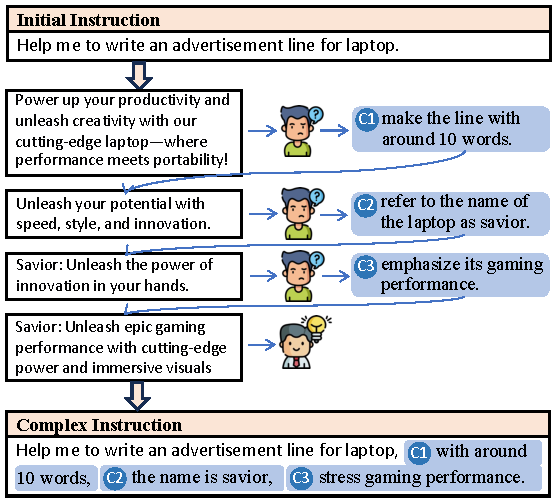
\includegraphics[width=0.5\textwidth]{source/intro.pdf}
\end{graphicalabstract}

\begin{highlights}
\item DIR derives complex instructions from unstructured human documents.
\item Iterative refinement grounds constraints in document content and model errors.
\item Constraint-aware SFT and RL jointly improve instruction following.
\item DIR improves FollowBench HSR and AlpacaEval 2.0 over existing baselines.
\end{highlights}

\begin{keywords}
Complex instruction \sep Instruction following \sep LLM alignment \sep Large language models
\end{keywords}

\maketitle

\section{Introduction}

Recent advancements in Large Language Models (LLMs) have shown impressive performance across a wide range of tasks~\citep{zhao2023survey, li2024graphreader, he2024chinesesimpleqa}. Driven by vast amounts of data and efficient training, state-of-the-art LLMs demonstrate robust capabilities in following general instructions and achieving alignment with human preferences~\citep{ouyang2022training,li20242d,huang2025musc}.
However, despite these successes, they still face significant challenges when it comes to complex instruction following~\citep{jiang2023followbench,wen2024benchmarking}, which requires simultaneous satisfaction of multiple constraints. The ability to reliably execute such complex instructions is fundamental for LLMs to be deployed in sophisticated real-world scenarios, where user intent is inherently nuanced and multi-faceted.

High quality instruction data is essential for instruction alignment. Existing datasets of complex instructions primarily originate from two sources: 1) Curated data from open-source datasets or human annotations~\citep{zhou2024lima,zhang2024cfbench}, which are resource-intensive and \textbf{lacking scalability}, and 2) Transforming simple instructions into complex ones automatically using proprietary LLMs~\citep{xu2023wizardlm,sun2024conifer}. 
While the automatic methods improve scalability, the generated constraints are often recombinations of few-shot examples, resulting in \textbf{limited diversity}.
Moreover, these constraints may have \textbf{low relevance} to the target output, failing to reflect real-world scenarios, as they are derived without considering the actual response's deficiencies.

\begin{figure}[pos=t]
    \centering
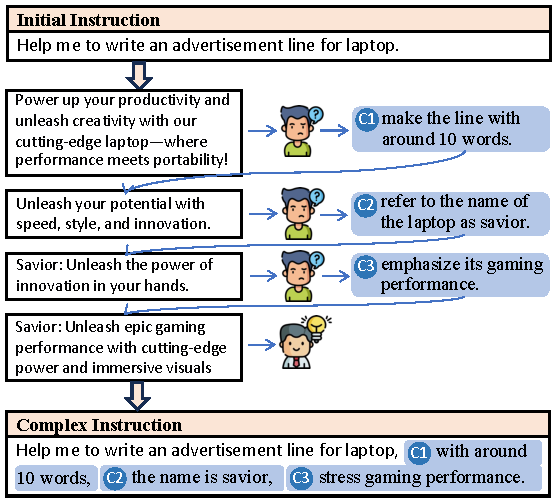
\includegraphics[width=0.86\linewidth]{source/intro.pdf}
    \caption{An illustration of humans iteratively refining instructions for higher complexity to better align with human preference.}
    \label{fig: intro}
\end{figure}

% where human iteratively refine instructions to be more complex, as shown in Figure \ref{fig: intro}.

Recently, back-translation, which involves translating text from the target response back into the source instruction, has been proposed to generate scalable and diverse instructions from human-written corpora~\citep{sennrich2015improving,hoang2018iterative,zheng2024kun,li2023self}. 
% Some studies have explored how back-translation can be leveraged to better generate instructions for fine-tuning large models~\cite{li2023self,zheng2024kun,nguyen2024better}. 
However, these methods typically focus on generating \textbf{simple instructions}, and one-way back-translation cannot fully explore the rich knowledge contained in the human corpus.

% To address the scalability and diversity of producing complex instructions,
In this paper, we propose a \textbf{Document-grounded Iterative Refinement (DIR)} framework for generating high-quality complex instructions.
Specifically, our approach is based on two key observations. First, human-written documents contain massive human preferences that can be converted into specific constraints, such as formatting conventions. Second, humans often refine complex instructions iteratively based on feedback from model outputs. As illustrated in Figure~\ref{fig: intro}, simple instructions are progressively adjusted and enriched to better align with human preferences. This iterative process plays a critical role in crafting effective complex instructions.

Therefore, our DIR framework incorporates both document-based knowledge and iterative judgment process to construct complex instructions. 
The framework consists of two key steps: 1) \textbf{Initial Instruction Generation}, where the model generates initial instructions based on the document content; 2) \textbf{Iterative Instruction Refinement}, where instructions are iteratively refined with LLM-as-judge guidance by comparing model outputs with the document, to identify and incorporate valuable constraints. This process enables us to generate more challenging instructions that align more closely with real-world scenarios. With this approach, we have curated \textbf{DIR-10K}, a high-quality complex instruction dataset.

Building upon this data, we further propose a \textbf{constraint-aware optimization pipeline} to effectively achieve instruction alignment. First, we perform Supervised Fine-Tuning (SFT) on complex instruction-response pairs curated by LLM-as-judge. Second, we employ constraint-aware Reinforcement Learning (RL) with a hybrid reward system: a model-based reward for soft constraints and a rule-based reward for hard constraints. Notably, the reward model is trained by leveraging response pairs generated during the iterative refinement process, and therefore does not require additional annotation. 

We validate our approach across various models. Experimental results demonstrate that our approach achieves significant improvements in both general and complex instruction-following tasks, thereby verifying its effectiveness. 

In summary, our contributions are as follows: 

\begin{itemize}[leftmargin=4mm]
    \item We propose the \textbf{DIR} framework, which leverages an LLM-as-judge mechanism to iteratively refine complex instructions by comparing with human-crafted documents.
    
    \item We release \textbf{DIR-10K}, a high-quality complex instruction dataset curated via our framework that achieves better alignment with real-world requirements. 
    
    \item We develop a \textbf{constraint-aware optimization pipeline} (SFT+RL) featuring a hybrid reward system that effectively aligns LLMs with complex constraints.
    
    \item Empirical results demonstrate that our fine-tuned models significantly outperform existing state-of-the-art methods across multiple instruction-following benchmarks.
\end{itemize}
\section{Related Work}
\subsection{Complex Instruction Generation}

% Instruction tuning is essential for aligning Large Language Models (LLMs) with user intentions. Initial endeavors in this field primarily focused on the curation and refinement of existing open-source NLP datasets \cite{wang2023far,ding2023enhancing}. With the importance of instruction quality recognized, manual annotation methods emerged~\cite{wang2023far,zhou2024lima}.

Instruction tuning is essential for aligning LLMs with user intentions~\citep{ouyang2022training,cao2023instruction}. Initial efforts in this domain focused on constructing instruction-following datasets through three primary channels: 1) adapting existing NLP benchmarks into instruction formats~\citep{longpre2023flan,wang2022super}; 2) manual curation via crowdsourcing~\citep{DatabricksBlog2023DollyV2, kopf2023openassistant}; and 3) distilling responses from proprietary models~\citep{alpaca, vicuna2023}. While these methods provide high-quality responses, they often fail to capture the complexity of real-world user queries. Therefore, the automated synthesis of complex instructions has emerged as a challenge.

Several strategies have been proposed to address the scarcity of complex instructions. For instance, Evol-Instruct \citep{xu2023wizardlm} employed LLMs to incrementally increase the depth and breadth of instructions through constraints, deepening, and concretizing. Similarly, Conifer \citep{sun2024conifer} utilized a multi-level taxonomy to inject fine-grained constraints into instructions. However, these methods primarily rely on few-shot prompting, which often results in synthetic constraints that diverge from the natural distribution of complex instructions in real applications.

Back-translation, a process of translating text from the target language back into the source language, is mainly used for data augmentation in tasks like machine translation~\citep{sennrich2015improving, hoang2018iterative}.  \citet{li2023self} first applied this to large-scale instruction generation using unlabeled data, with Suri~\citep{pham2024suri} and Kun~\citep{zheng2024kun} extending it to long-form and Chinese instructions, respectively. \citet{nguyen2024better} enhanced this method by adding quality assessment to filter and revise data. Building on this, we further investigated methods to generate high-quality complex instruction datasets using back-translation in an iterative manner.

\subsection{Complex Instruction Alignment}

Alignment methods are essential for enhancing complex instruction-following capabilities. Early approaches primarily relied on Supervised Fine-Tuning (SFT) using data distilled from stronger models \citep{xu2023wizardlm, sun2024conifer}. For instance, WizardLM \citep{xu2023wizardlm} utilized an iterative strategy to construct training data for SFT. I-SHEEP \citep{isheep} introduced an SFT strategy based on an active self-enhancement paradigm where the model aligns itself. However, the inherent limitations of imitation learning often constrain the overall performance of these methods \citep{gudibande2023falsepromiseimitatingproprietary}.

Recent studies also employ Direct Preference Optimization (DPO) on preference pairs, where negative samples are misaligned with the complex instruction \citep{huang2025musc, he2024complex, pham2024suri}. These methods either rely on automatic response detachment \citep{huang2025musc,ren2025step} or rule-based verification \citep{guo2025recast} to construct misaligned responses. However, the efficacy of DPO is often limited because negative samples frequently originate from models with different parameter distributions from the target model, leading to optimization bottlenecks \citep{ivison2024unpacking}. Therefore, other studies also started to employ online reinforcement learning methods to mitigate the distribution drift \citep{ren2026lsriflogicstructuredreinforcementlearning,qin2025incentivizingreasoningadvancedinstructionfollowing}. Nevertheless, the lack of high-quality reward signals remains a major hurdle for online optimization. Developing more efficient strategies for complex instruction alignment remains a critical problem.
\section{Complex Instruction Generation}
The complex instruction generation framework \textbf{DIR} mainly consists of two steps: 1) Initial Instruction Generation, 2) Iterative Instruction Refinement, as shown in Figure \ref{fig:main}.
% \footnote{An end-to-end case study of this pipeline is illustrated in Appendix A-A.} In this section, we will introduce the two steps in detail.


\begin{figure*}[pos=tbp]
    \centering % 将图居中
    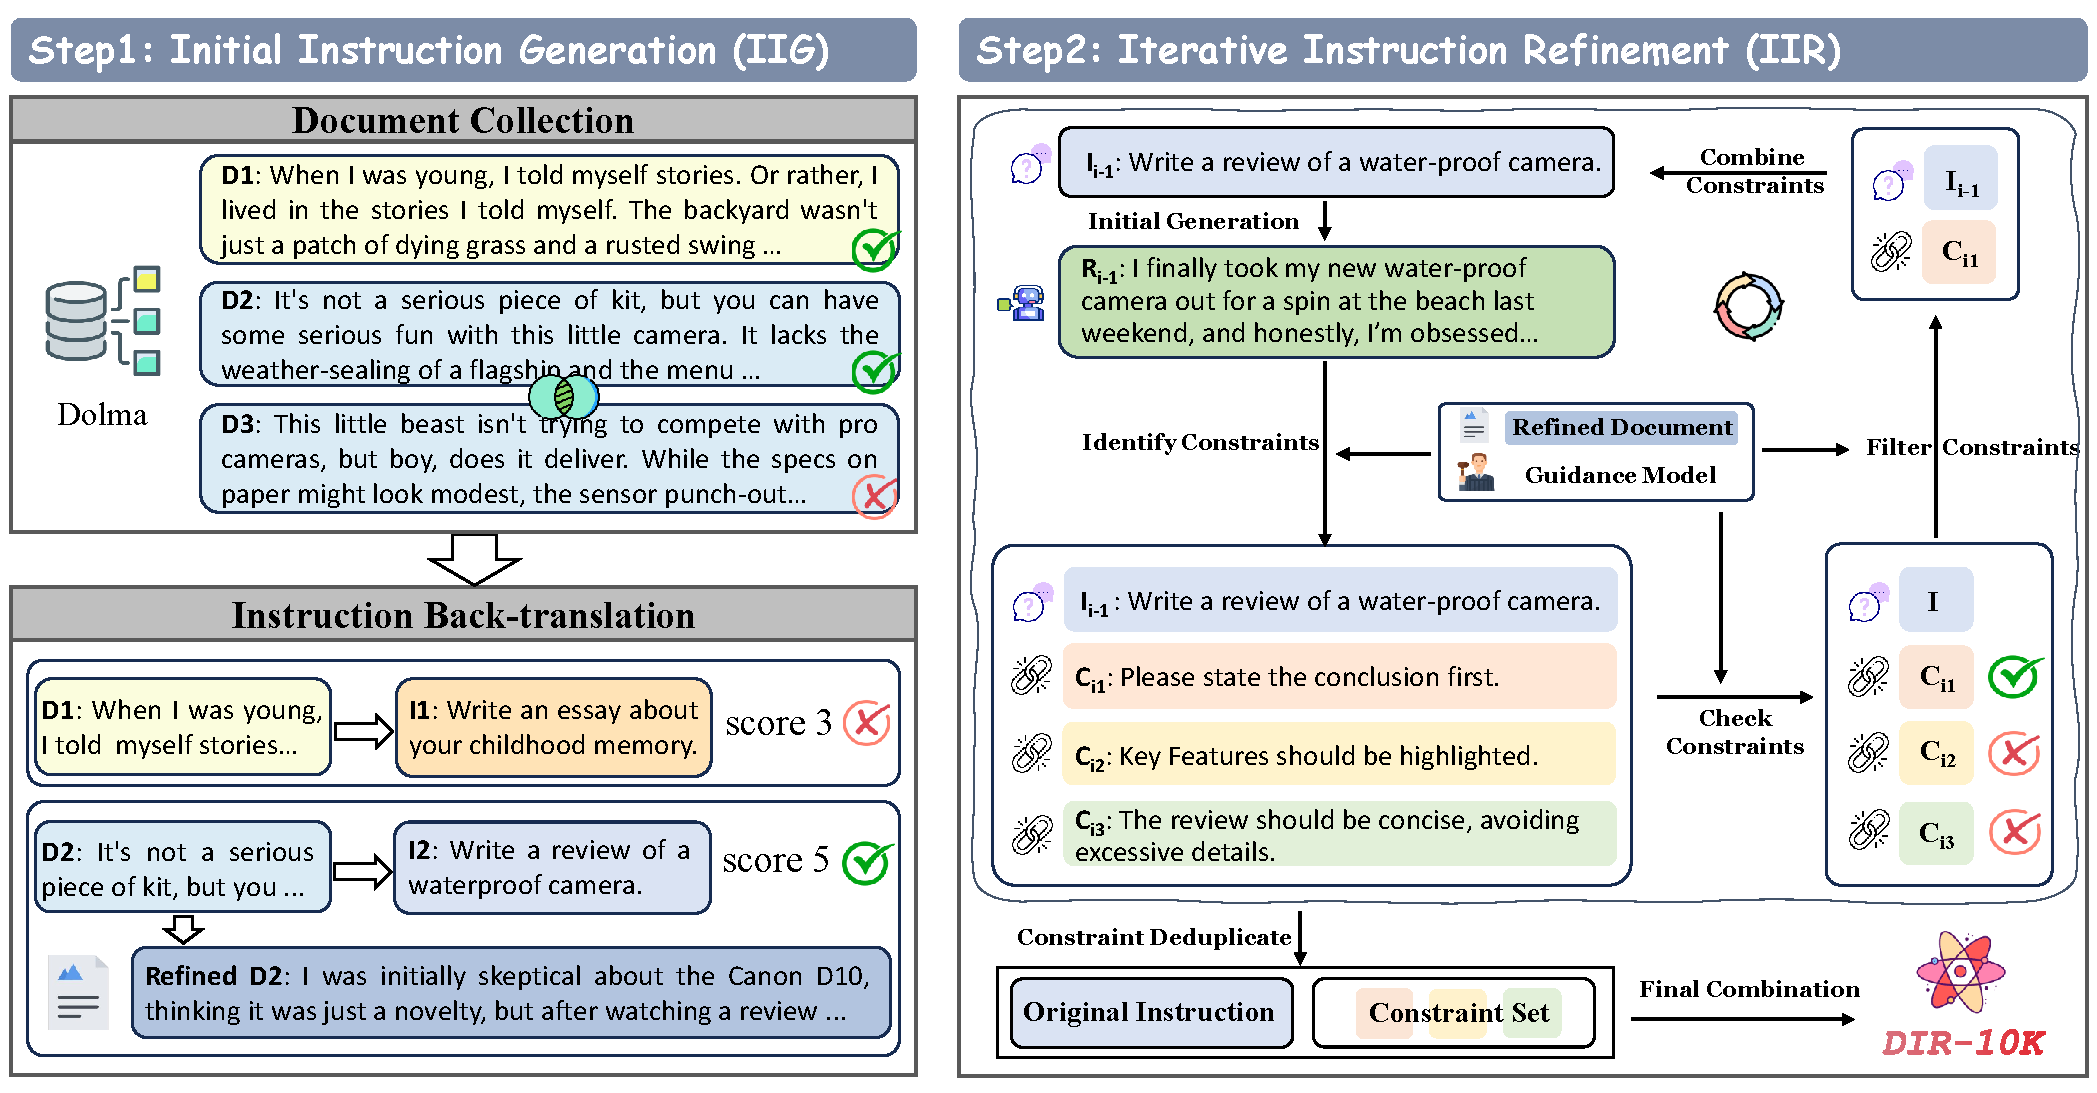
\includegraphics[width=1.0\linewidth]{source/main.pdf}
    \caption{
     DIR: Document-grounded Iterative Refinement. In the IIG phase, a large number of documents are collected for deduplication, followed by quality filtering based on scores assigned by the guidance model. Initial instructions are then generated using back-translation. In the IIR phase, refined documents and model responses from each iteration are used to generate constraints, ensuring compliance with the requirements stated in Section \ref{sec:IIR}. This iterative process continues until a final constraint set is produced, which is further combined with the original instruction to form the ultimate instruction.
    }
    \label{fig:main}
\end{figure*}

\subsection{Initial Instruction Generation (IIG)}

\subsubsection{Document Collection}
\label{sec:document_collection}
Traditional instruction generation methods such as Self-Instruct \citep{wang2022self} often suffer from limited diversity, as the generated instructions are generally re-combinations of the provided few-shot examples. Therefore, we propose a novel back-translation approach to construct initial instructions based on human-written documents.

To ensure the diversity of the generated instructions, we implement a density-based sampling mechanism for documents, as shown in Algorithm \ref{Alg:density}. Specifically, we convert documents into vector representations using Sentence-Transformers\footnote{\texttt{sentence-transformers/all-MiniLM-L6-v2}.}, and perform sampling to maximize the density of samples in the representation space. In this way, we effectively eliminate redundant documents. Furthermore, this approach ensures that the knowledge introduced in the instructions is evenly distributed across various domains, which prevents the model from overfitting to a specific domain and mitigates the risk of catastrophic forgetting of fundamental capabilities. 

Additionally, to further ensure the quality of the document collection, we filter out documents based on the following criteria: 1) Length: Remove documents with fewer than 50 words or exceeding 2,048 words; 2) Symbol ratio: Remove documents where the proportion of symbols exceeds that of textual content; and 3) Redundancy: Remove documents containing repetitive paragraphs or excessive symbol repetitions.


\begin{algorithm}[t]
  \renewcommand{\algorithmicrequire}{\textbf{Input:}}
  \renewcommand{\algorithmicensure}{\textbf{Output:}}
  \caption{Density-based Document Sampling}
  \begin{algorithmic}[1]
      \REQUIRE Initial collection $D$ with $m$ documents, number of documents to select $n$. 
      \ENSURE Selected collection $D'$ with $n$ documents.
      \STATE Derive the embeddings for each document in $D$.
      \STATE Randomly sample one document $x$ from $D$.
      \STATE Delete $x$ from $D$, add $x$ to $D'$.
      \FOR{$i = 1, 2, ..., n-1$}
          \STATE Calculate the cosine similarity score between $x$ and each document from $D$.
          \STATE Select the least similar document $x'$ from $D$.
          \STATE Let $x$ = $x'$.
          \STATE Delete $x$ from $D$, add $x$ to $D'$. 
      \ENDFOR
  \end{algorithmic}
\label{Alg:density}
\end{algorithm}

\subsubsection{Instruction Back-translation}
Based on the sampled documents, we employ a back-translation \citep{li2023self} method to construct initial instructions. Specifically, we utilize a proprietary guidance model\footnote{The guidance model is a proprietary LLM that is significantly stronger than the base model, as detailed in Section \ref{sec:models}.} to predict an instruction that can be answered with the document. This enables the generation of new instructions without relying on few-shot examples or pre-designed rules. Moreover, we can further ensure the diversity of the generated instructions by diversifying the documents.

Despite being derived from documents, the instructions do not always align well with the original document for two reasons. First, the documents are unstructured and do not conform to the AI-assistant format. Second, the documents may contain information irrelevant to the instruction ~\citep{nguyen2024better}. Therefore, we introduce a refinement step to transform the documents into response format and remove irrelevant content.

To further ensure data quality, we introduce a scoring step to filter out low-quality instructions. Each instruction is assigned a score on a scale of $1$ to $5$ by the guidance model, with each point corresponding to a specific dimension. Only instructions with a score of 4 or above are retained for the next step.

% \footnote{Instruction score criteria are presented in Appendix \ref{appendix:ins_score_case}.}

\subsection{Iterative Instruction Refinement (IIR)}
\label{sec:IIR}
To enhance a model’s ability to follow complex instructions, it is crucial to construct complex instruction data with multi-faceted constraints. Previous methods typically start with simple instructions and generate complex ones through rewriting~\citep{xu2023wizardlm}. However, the constraints generated in this way often do not meet actual needs or lack diversity.

% Therefore, we iteratively refine instructions by emulating the real-world process where people iteratively review responses and add constraints to address their deficiencies. This approach helps in developing more effective and challenging instructions.

% In practice, constructing complex instructions usually involves iteratively reviewing the response and adding constraints to address its deficiencies.

An effective sample for complex instruction alignment should adhere to two key principles:

\begin{enumerate}[itemsep=1mm, parsep=0pt]
    \item Whether the model’s response originally misaligns with the constraint before it is added;
    \item Whether the model’s response still misaligns with the constraint after it is added.
\end{enumerate}

These constraints highlight the model’s weaknesses in handling complex instructions and require further improvement. Conversely, if a constraint does not meet these principles, it indicates that the constraint falls within the model’s current capabilities and does not require additional learning.

Therefore, we introduce constraint generation using LLM-judge guidance \citep{zheng2023judging}, which mimics the human process of iteratively refining prompts to form complex instructions. During the iteration process, this method leverages the guidance model to judge the current response and identifies the constraints that the model fails to satisfy, thereby expanding simple instructions into complex ones, as shown in Algorithm \ref{alg:iir}.

% With the refined document as $R$, this method expands simple instructions $Q_o$ into complex ones through the following steps\footnote{Detailed prompt templates are presented in Appendix \ref{appendix:prompt_iir}.}:

\begin{figure*}[pos=tbp]
\centering
\includegraphics[width=0.96\linewidth]{source/iteration_constraint_distribution.png}
\caption{Constraint type distribution on DIR-10K among different iterations.}
\label{figure:constraint_dist}
\end{figure*}

\begin{algorithm}[t]
  \renewcommand{\algorithmicrequire}{\textbf{Input:}}
  \renewcommand{\algorithmicensure}{\textbf{Output:}}
  \caption{Iterative Instruction Refinement}
  \label{alg:iir}
  \begin{algorithmic}[1]
      \REQUIRE Guidance model $M$, current model $m$, refined document $D$, initial instruction $I_0$.
      \ENSURE Constraint Sets $C_n$ and $C_n'$.
      \FOR{$i = 1, 2, ..., n$}
          \STATE Use $m$ to generate a response $R_i$ for the previous instruction $I_{i-1}$.
          \STATE Leverage $M$ as the judge, compare $R_i$ with $D$ to identify a new constraint $c_i$.
          \STATE Add $c_i$ to $C_n$.
          \STATE Add $c_i$ to $I_{i-1}$ to form a new instruction $I_i$.
          \STATE Use $m$ to generate a response $R_{i}'$ for $I_i$.
          \STATE Leverage $M$ as the judge, check whether $R_i'$ satisfies constraint $c_i$. If not, add $c_i$ to $C_n'$. 
      \ENDFOR
  \end{algorithmic}
\end{algorithm}

% \begin{enumerate}[itemsep=1mm, parsep=0pt]
%     \item Leverage current model to generate a answer $A_i$ for the instruction $Q_i$.
%     \item Leveraging a guidance model as the judge, compare the refined document $R$ with the model's response to identify a new constraint $c_i$.
%     \item Add the constraints to the question $Q_{i-1}$ to construct a new question $Q_i$.
%     \item Answer $Q_i$ using the current model to derive answer $A_i$.
%     \item Determine whether the constraint $C_i$ is satisfied by $A_i$. If not, add the constraint to $C_n$.
%     \item Repeat the above three steps for multiple rounds to uncover increasingly complex constraints, thereby increasing the difficulty and depth of the instructions.
% \end{enumerate}

Throughout the iterative judgment process, as the number of constraints increases, the model's response also improves, making the identification of new constraints more challenging. Therefore, we utilize the refined document as the reference answer for judgment. Human-written documents inherently contain vast amounts of knowledge and formatting conventions that reflect human preferences. By grounding the constraint-generation process in documents, we achieve constraints that align more closely with human preferences.

Finally, the constraint set is merged into a new instruction. Note that two constraint sets are derived: the first set $C_n$ satisfies Principle 1, while the second set $C_n'$, which includes an additional checking step, satisfies both Principle 1 and 2.
% \footnote{An example of the IIR process is presented in Appendix \ref{appendix:pipeline_case}.}
% \textcolor{red}{Notice our approach incorporates several measures to ensure efficiency and scalability when handling large-scale documents and multiple iterations, while demonstrating robustness to variations in document quality, as detailed in Appendix \ref{appendix:efficiency_scalability} and \ref{appendix:document_quality}.}



\subsection{Data Statistics of DIR-10K}

\begin{figure}[pos=htbp]
\centering
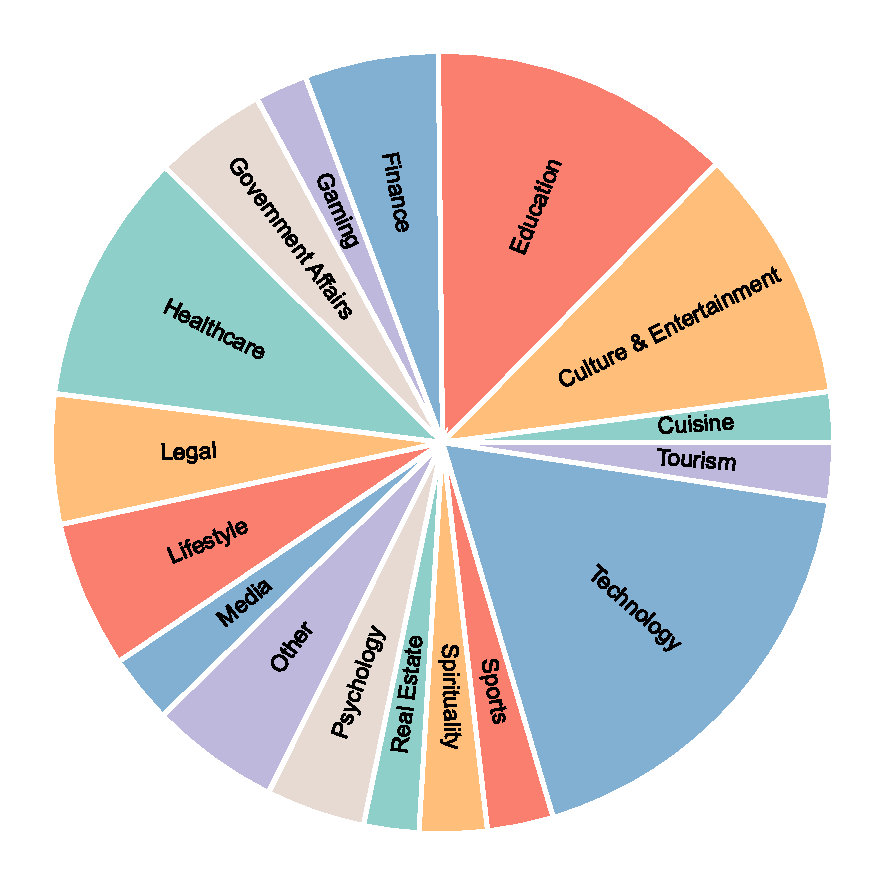
\includegraphics[width=0.6\linewidth]{source/data_visualization/domain_distribution.pdf}
\caption{Domain distribution on DIR-10K.}
\label{figure:domain_dist}
\end{figure}

\begin{figure}[pos=htbp]
\centering
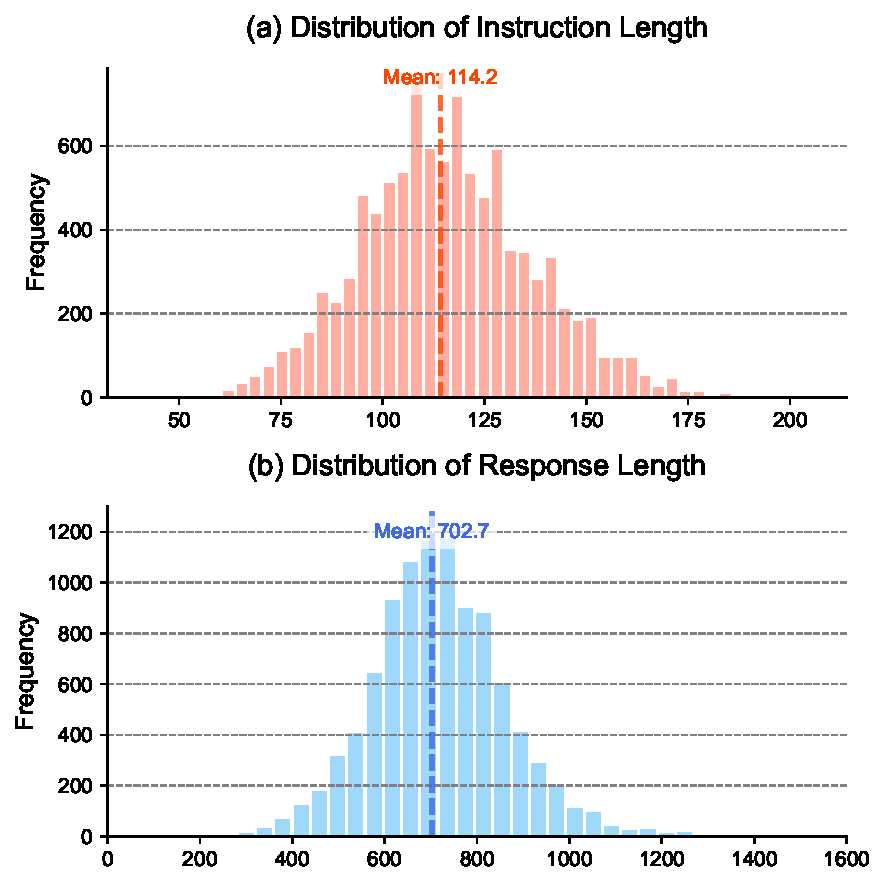
\includegraphics[width=0.78\linewidth]{source/data_visualization/length_distribution.pdf}
\caption{Distribution of instruction and response length on DIR-10K.}
\label{figure:length_dist}
\end{figure}

Utilizing our proposed framework, we constructed a high-quality complex instruction dataset, \textbf{DIR-10K}, based on openly available documents\footnote{We use a subset of Dolma v1.7 \citep{dolma-2024} following \citet{nguyen2024better}.}. Figure \ref{figure:constraint_dist} illustrates the evolution of constraint distributions across iterations (where a specific constraint type is specified for each generation). As can be seen, while \textit{Inclusion} and \textit{Document Structure} constraints predominate in the initial iteration, the distribution becomes progressively more uniform as iterations proceed. This validates that by uncovering constraints which are not covered by previous refinement iterations, our iterative refinement process effectively ensures constraint diversity.

We also present the domain distribution of DIR-10K in Figure \ref{figure:domain_dist}, following the domain definition in CFBench \citep{zhang2024cfbench}. As shown, our dataset encompasses nearly 20 different domains, exhibiting a high degree of balance across diverse fields. Furthermore, we analyzed the length distribution of the instructions using \textit{tiktoken}\footnote{We used \textit{o200k\_base} tokenizer for length calculation.}. As shown in Figure \ref{figure:length_dist}, the instruction lengths are primarily concentrated between 75 and 150 tokens, while the response lengths can scale to around 700 tokens, ensuring that our instructions provide sufficient information for aligning with complex instructions.
\section{Constraint-aware Optimization}
\label{sec:optimization}

\begin{figure*}[pos=tbp]
    \centering % 将图居中
    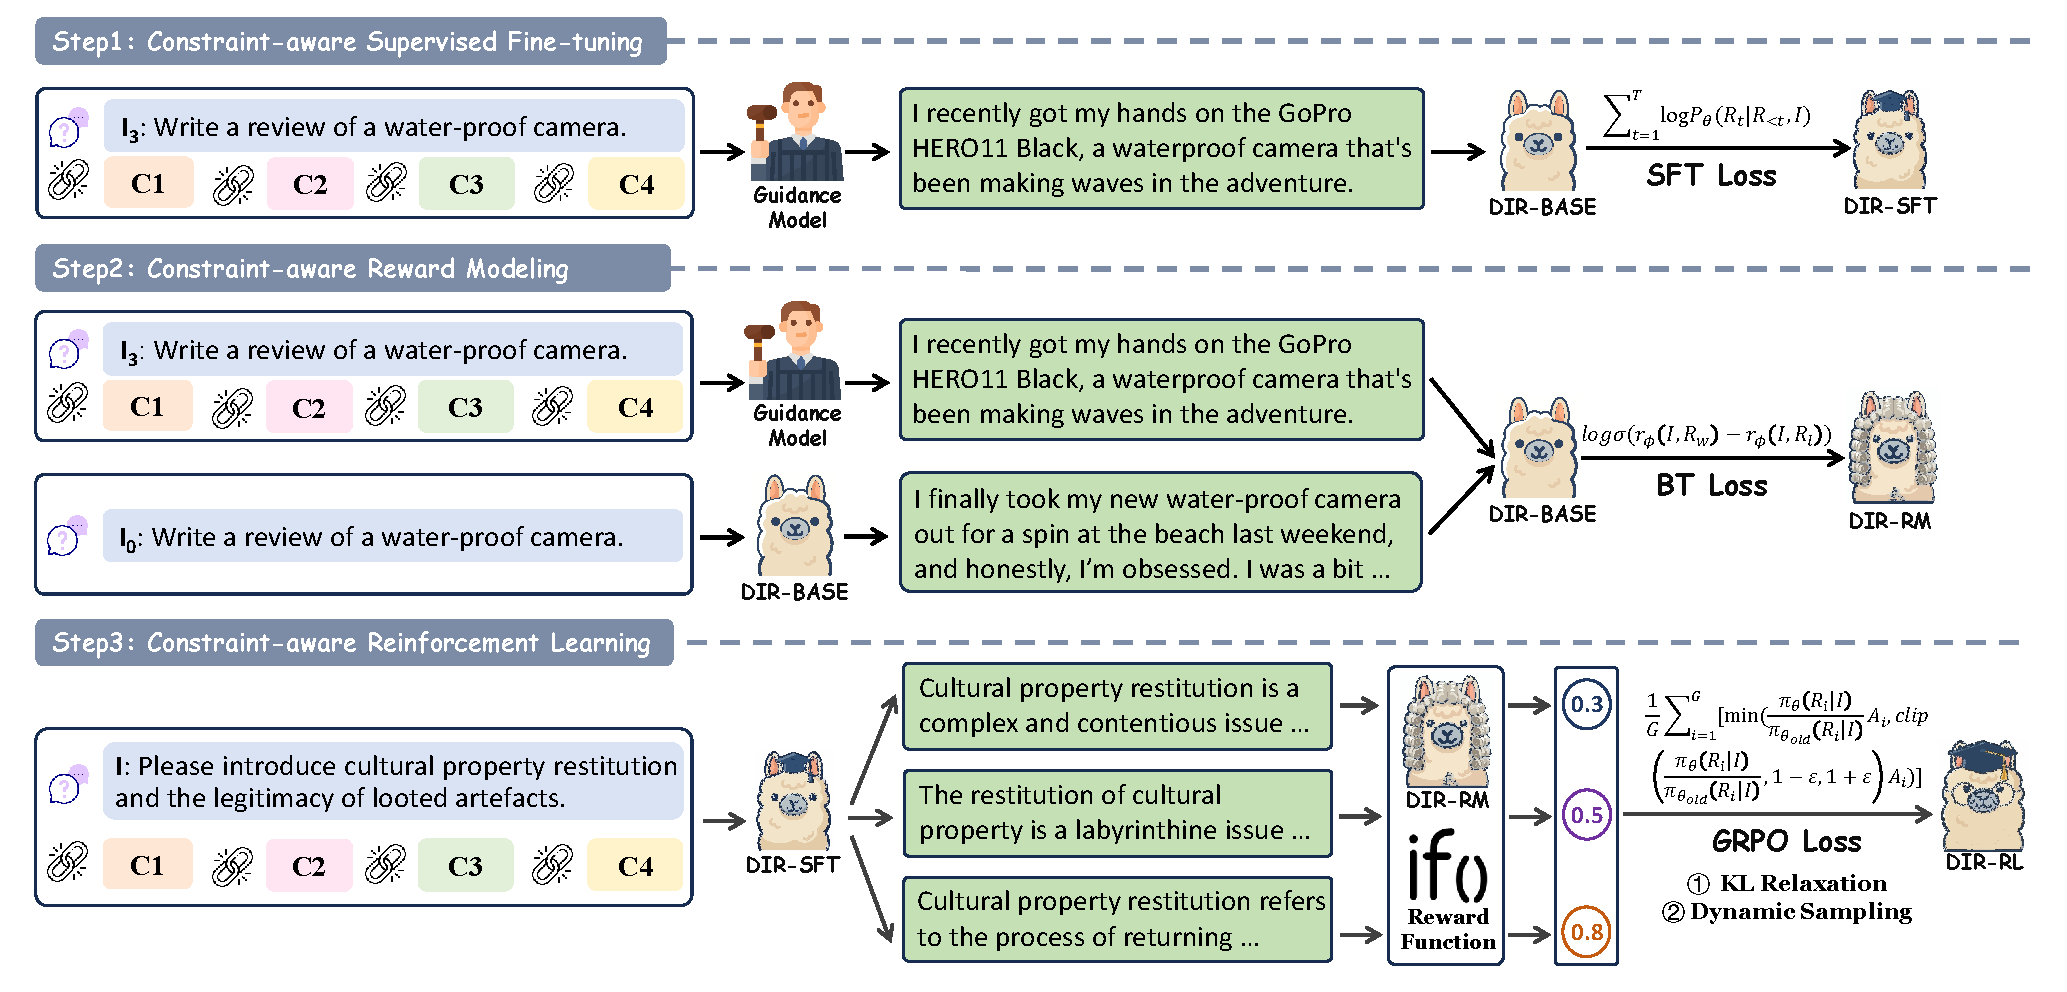
\includegraphics[width=1.0\linewidth]{source/main_RL.pdf}
    \caption{
     The Illustration of Constraint-aware Optimization. We first perform Constraint-aware SFT on responses curated by the guidance model. Then we leverage intermediate responses generated during the iterative process as negative samples, to train the Constraint-aware Reward Model (RM). Finally, we conduct Constraint-aware Reinforcement Learning, guided by a hybrid feedback mechanism that integrates both the neural RM and rule-based rewards.
    }
    \label{fig:main_rl}
\end{figure*}

Building upon the high-quality instruction data \textbf{DIR-10K}, we present a constraint-aware optimization pipeline to enhance the instruction-following capabilities of LLMs, as illustrated in Figure \ref{fig:main_rl}. This method mainly consists of two steps, as in the following sections.

\subsection{Constraint-aware Supervised Fine-tuning}

The first stage involves Supervised Fine-Tuning (SFT) \citep{ouyang2022training} using the standard negative log-likelihood (NLL) loss:

\begin{equation}
\begin{aligned}
\mathcal{L}_{SFT}(\theta) & = \\
& \quad -\sum_{t=1}^{T} \log P_{\theta}(R_t \mid R_{<t}, I)
\end{aligned}
\end{equation}

\noindent where $I$ represents the complex instruction and $R$ denotes the curated response. Since our instructions are iteratively refined to incorporate diverse real-world constraints, this stage enables the model to establish a foundational mapping between complex instructions and desired outputs.

Notably, while the refined document serves as the basis for the judgment process, it is not used as the target for fine-tuning, as the document itself may not explicitly align with the newly introduced constraints~\citep{nguyen2024better}. Instead, we leverage the guidance model to generate responses based on the combined instructions, ensuring that the model is optimized on responses that strictly adhere to the specified constraints.

\subsection{Constraint-aware Reinforcement Learning}
\label{sec:rl}

While SFT effectively initiates the model with complex instruction-following capabilities, it faces three critical bottlenecks: \textbf{1) Lack of Negative Supervision:} SFT focuses solely on maximum likelihood estimation of positive samples, failing to provide the explicit penalties necessary to suppress undesirable behaviors \citep{gudibande2023falsepromiseimitatingproprietary}. This prevents the model from associating constraint violations with performance degradation. \textbf{2) Teacher-bounded Performance:} The model's performance is inherently capped by the quality of the reference response generated by the guidance model. This restricts the model from exploring more optimal response strategies that might surpass the teacher's initial output. \textbf{3) Sparse Reward Signals:} Many complex constraints (e.g., inclusion constraint, length constraint) are discrete and non-differentiable, making them ill-suited for SFT’s token-level cross-entropy loss.

To bridge these gaps, we propose constraint-aware Reinforcement Learning (RL) that transitions from pattern imitation to direct constraint alignment. The RL is based on a hybrid reward system as follows.

\subsubsection{Model-based Reward}

For subjective constraints such as sentiment and tone, we train a discriminative reward model $r_\phi$ using the Bradley-Terry objective:

\begin{equation}
\begin{aligned}
\mathcal{L}_{RM}(\phi)
&= -\mathbb{E}_{(I, R_w, R_l) \sim \mathcal{D}_{pref}}
\left[ \log \sigma \left( r_\phi(I, R_w) \right.\right. \\
&\hspace{5.7em}\left.\left.{} - r_\phi(I, R_l) \right) \right]
\end{aligned}
\end{equation}

\noindent where $R_w$ and $R_l$ are the chosen and rejected responses.

We leverage the iterative nature of the DIR framework to construct high-quality preference pairs $(I, R_w, R_l)$. As shown in Algorithm \ref{alg:iir}, during the IIR process, the guidance model identifies specific deficiencies in the response from a previous iteration ($R_i$) and proposes incremental constraints to rectify them. Consequently, $R_i$ naturally serves as the rejected sample $R_l$, while the refined response from the guidance model acts as the chosen sample $R_w$. By training on these pairs, the reward model effectively internalizes instruction following and learns to assign higher scores to responses that satisfy sophisticated constraints.
%, thereby providing a robust guidance signal for the subsequent RL process.

To mitigate the potential degradation of general capabilities during reinforcement learning, we augment the preference data with samples from the \textit{Skywork-Reward-Preference-80K-v0.2} dataset \citep{liu2025skywork} at a 1:1 ratio. This balanced mixture ensures that the reward model maintains a robust assessment of both general and complex instruction alignment.

\subsubsection{Rule-based Reward}
For verifiable hard constraints (e.g., length, keyword inclusion), we employ automated scripts to generate a binary signal $V(\mathbf{c}, R) \in \{0, 1\}$, where $\mathbf{c}$ denotes the set of hard constraints specified in $I$. To prioritize these hard constraints over stylistic nuances, we implement a Constraint-prioritized Reward Fusion strategy:

\begin{equation}
\mathcal{R}(I, R) =
\begin{cases}
\sigma(r_\phi(I, R)) & \text{if } \mathbf{c} = \varnothing \\
0.5 + 0.5 \cdot \sigma(r_\phi(I, R)) & \text{if } V(\mathbf{c}, R) = 1 \\
0.5 \cdot \sigma(r_\phi(I, R)) & \text{if } V(\mathbf{c}, R) = 0
\end{cases}
\end{equation}

This piecewise mapping ensures that any response failing hard constraints ($V=0$) receives a strictly lower score (range $[0, 0.5]$) than those satisfying them ($V=1$, range $[0.5, 1.0]$).

\subsection{Optimization with GRPO}

Based on the hybrid reward system, we utilize Group Relative Policy Optimization (GRPO) \citep{shao2024deepseekmath} to perform RL. To better adapt GRPO to complex instruction-following tasks, we introduce two key modifications:

\begin{enumerate}[leftmargin=4mm]
    \item \textbf{KL-Penalty Relaxation:} Unlike traditional RLHF where RL objectives may diverge from the SFT distribution, our SFT and RL stages share the unified goal of instruction following, and the risk of representation collapse is significantly reduced \citep{parthasarathi2025grpolambdacreditassignmentimproves}. Therefore, we omit the explicit KL-penalty term from the loss function, relying instead on the PPO-style clipping mechanism for stability \citep{hu2025openreasonerzeroopensourceapproach}. This relaxation allows for more aggressive exploration and closer alignment with complex constraints.
    \item \textbf{Dynamic Sampling Mechanism:} As the policy optimizes, standard uniform sampling frequently encounters saturated groups where all responses satisfy the constraints, resulting in uninformative reward differences \citep{yu2025dapo}. To maintain optimization efficiency, we implement a mechanism that evaluates the within-group reward standard deviation, and if the deviation falls below a predefined threshold $\tau$, the query is identified as lacking sufficient discriminative signal and is dynamically excluded from the optimization step.
\end{enumerate}

Based on the two modifications, the optimization objective during our RL phase is as follows:

\begin{equation}
\begin{split}
\mathcal{L}_{GRPO}(\theta) & = \frac{1}{G} \sum_{i=1}^{G} \bigg[ \min \Big( \frac{\pi_{\theta}(R_i|I)}{\pi_{\theta_{old}}(R_i|I)} \mathcal{A}_i, \\
& \text{clip}\left( \frac{\pi_{\theta}(R_i|I)}{\pi_{\theta_{old}}(R_i|I)}, 1-\epsilon, 1+\epsilon \right) \mathcal{A}_i \Big) \bigg]
\end{split}
\end{equation}

\noindent where for each instruction $I$, we sample a group of outputs $\{R_i\}_{i=1}^G$, and the advantage $\mathcal{A}_i$ is computed by normalizing the rewards $\mathcal{R}(I, R_i)$ within the group:

\begin{equation}
\mathcal{A}_i = \frac{\mathcal{R}(I, R_i) - \text{mean}(\mathcal{R}(I, R_1), \dots, \mathcal{R}(I, R_G))}{\text{std}(\mathcal{R}(I, R_1), \dots, \mathcal{R}(I, R_G))}
\end{equation}

By incorporating explicit penalties for constraint violations, the RL framework provides a holistic evaluation signal that enables the model to distinguish between compliant and non-compliant responses, thereby enhancing its instruction following ability for both general and complex instructions.
\section{Experiments}
\subsection{Set-up}

\subsubsection{Data} 
Following \citet{nguyen2024better}, we utilize a subset of Dolma v1.7 \citep{dolma-2024} as the document source, which is derived from a collection of web pages and has undergone rigorous quality and content filtering to ensure data quality.

\subsubsection{Models} 
\label{sec:models}
We apply our method to two models, Llama-3-8B and Qwen2.5-7B, and we apply preliminary supervised fine-tuning to both models. The preliminary fine-tuning process is conducted on two general instruction datasets, namely ultrachat-200k \citep{ding2023enhancing} and tulu-330k \citep{lambert2024tulu3}, respectively. For the guidance model, we rely on a larger model from the same family to ensure data quality, namely Qwen-2.5-72B-Instruct for Qwen-2.5-7B, and Llama-3-70B-Instruct for Llama-3-8B. We set the maximum number of iterations to 5.

\subsubsection{Evaluation} 
We mainly conduct evaluations on two complex instruction-following benchmarks, \textbf{CFBench}~\citep{zhang2024cfbench} and \textbf{FollowBench}~\citep{jiang2023followbench}, where instructions consist of multiple constraints. We also conduct evaluations on a general instruction benchmark of \textbf{AlpacaEval2}~\citep{dubois2024length}. Note that we use GPT-4o-0806 \footnote{\url{platform.openai.com/docs/models/gp\#gpt-4o}} as the evaluator for all of benchmarks. 

\subsubsection{Baselines}
We mainly compare with the following methods of complex instruction generation and alignment:

\begin{enumerate}
    \item \textbf{ShareGPT}: This repository aggregates real-world, multi-turn human-AI dialogues to provide models with authentic and diverse interaction patterns.
    \item \textbf{Self-Instruct} \citep{wang2022self}: This framework utilizes a small set of human-written seeds to bootstrap the automatic generation of large-scale instruction datasets.
    \item \textbf{Evol-Instruct} \citep{xu2023wizardlm}: This method employs an evolutionary algorithm to iteratively rewrite simple instructions into more complex and diverse versions.
    \item \textbf{Muffin} \citep{lou2023muffin}: This approach scales task variety by generating multi-faceted instructions for the same input text to maximize the coverage of potential tasks.
    \item \textbf{Conifer} \citep{sun2024conifer}: This method refines datasets through an LLM-driven pipeline of query reframing and recombination to synthesize complex constraints.
    \item \textbf{ISHEEP} \citep{isheep}: This iterative paradigm enables models to generate and filter their own instruction-output pairs to improve alignment by self-enhancement.
    \item \textbf{Suri} \citep{pham2024suri}: This method uses instruction back-translation to derive complex prompts from high-quality human-written long-form texts for long-context training.
    \item \textbf{Crab} \citep{qi2024constraint}: This method retrofits existing instructions with constraints already satisfied by the responses to create challenging instruction data efficiently.
\end{enumerate}

    % \item \textbf{Human-crafted instruction data}: This includes ShareGPT\footnote{\url{huggingface.co/datasets/anon8231489123/ShareGPT_Vicuna_unfiltered}}, which is a collection of human-AI conversations.
    % \item \textbf{Automatically crafted general instruction data}: This includes Self-Instruct \cite{wang2022self}, which leverages few-shot examples to self-generate simple instruction samples.
    % \item \textbf{Automatically rewritten complex instruction data}: This includes Evol-Instruct \cite{xu2023wizardlm}, ISHEEP \cite{isheep}, Muffin \cite{lou2023muffin} and Conifer \cite{sun2024conifer}, which initiate with simple instructions and progressively construct more complex ones through rewriting or recombination.
    % \item \textbf{Automatically back-translated complex instruction data}: This includes Suri \cite{pham2024suri} and Crab \cite{qi2024constraint}, which curate the complex instructions and constraints by back-translating the pre-existing response. These methods are the closest to our work.

We also compare with the original methods of back-translation and back-and-forth translation  \citep{cao2023instruction, nguyen2024better}, where IIR is skipped and initial instructions are directly used. All methods are compared using 10k instruction-response pairs to ensure consistency.

\begin{table}[!t]
\centering
\caption{Hyper-parameters for SFT and GRPO experiments.}
\resizebox{0.38\textwidth}{!}{
\begin{tabular}{lc}
\toprule
\textbf{Configuration} & \textbf{Value} \\
\midrule
\multicolumn{2}{l}{\textit{Hyper-parameter setting for SFT}} \\
\midrule
Max Sequence Length     & 4096           \\
Learning Rate           & 1e-5           \\
LR Scheduler            & cosine decay   \\
Training Epochs         & 3              \\
Batch Size              & 64             \\
Mixed Precision         & bf16           \\
DeepSpeed ZeRO Stage    & stage 2        \\
\midrule
\multicolumn{2}{l}{\textit{Hyper-parameter setting for GRPO}} \\
\midrule
Generation Batch Size   & 512            \\
Training Batch Size     & 256            \\
Max Prompt Length       & 1024           \\
Max Response Length     & 4096           \\
Actor Learning Rate     & 3e-6           \\
Actor Mini Batch Size   & 64             \\
Actor Micro Batch Size  & 8              \\
KL Loss Coefficient     & 0.0            \\
Rollout Log Prob Batch Size & 16         \\
Rollout Number ($N$)    & 8              \\
Ref Log Prob Batch Size & 16             \\
Total Epochs            & 10             \\
\bottomrule
\end{tabular}
}
\label{tab:combined_hyperparams}
\end{table}


\begin{table*}[pos=tbp]
\centering
\caption{Main experiment results on Llama-3-8B-UltraChat, Llama-3-8B-Tulu and Qwen-2.5-7B-UltraChat.}
\setlength{\tabcolsep}{6pt}
\renewcommand{\arraystretch}{0.72}
\resizebox{0.90\textwidth}{!}{
\begin{tabular}{c|c|ccc|cc|cc}
\toprule
\multirow{2}{*}{\textbf{Base Model}} & \multirow{2}{*}{\textbf{Method}} & \multicolumn{3}{c}{\textbf{CF-Bench}} & \multicolumn{2}{c}{\textbf{FollowBench}} & \multicolumn{2}{c}{\textbf{AlpacaEval2}} \\
\cmidrule(lr){3-5} \cmidrule(lr){6-7} \cmidrule(lr){8-9}
& & \textbf{CSR} & \textbf{ISR} & \textbf{PSR} & \textbf{HSR} & \textbf{SSR} & \textbf{LC.Win} & \textbf{Len} \\
\midrule
\multirow{13}{*}{\makecell{\textbf{Llama-3-8B} \\ \textbf{-UltraChat}}} 
& Baseline & 0.51 & 0.15 & 0.22 & 41.04 & 57.39 & 8.86 & 1,017 \\ 
\cmidrule{2-9}
& Back-translation & $\text{0.40}_{\textcolor{deepred}{\text{-0.11}}}$ & $\text{0.11}_{\textcolor{deepred}{\text{-0.04}}}$ & $\text{0.15}_{\textcolor{deepred}{\text{-0.07}}}$ & $\text{21.19}_{\textcolor{deepred}{\text{-19.85}}}$ & $\text{33.92}_{\textcolor{deepred}{\text{-23.47}}}$ & $\text{0.96}_{\textcolor{deepred}{\text{-7.90}}}$ & 2,966 \\
& Back-and-forth & $\text{0.58}_{\textcolor{deepgreen}{\text{+0.07}}}$ & $\text{0.20}_{\textcolor{deepgreen}{\text{+0.05}}}$ & $\text{0.27}_{\textcolor{deepgreen}{\text{+0.05}}}$ & $\text{44.65}_{\textcolor{deepgreen}{\text{+3.61}}}$ & $\text{61.58}_{\textcolor{deepgreen}{\text{+4.19}}}$ & $\text{10.06}_{\textcolor{deepgreen}{\text{+1.20}}}$ & 1,440 \\
\cmidrule{2-9}
& ShareGPT & $\text{0.62}_{\textcolor{deepgreen}{\text{+0.11}}}$ & $\text{0.22}_{\textcolor{deepgreen}{\text{+0.07}}}$ & $\text{0.32}_{\textcolor{deepgreen}{\text{+0.10}}}$ & $\text{40.99}_{\textcolor{deepred}{\text{-0.05}}}$ & $\text{58.59}_{\textcolor{deepgreen}{\text{+1.20}}}$ & $\text{8.36}_{\textcolor{deepred}{\text{-0.50}}}$ & 1,052 \\
& Self-Instruct & $\text{0.34}_{\textcolor{deepred}{\text{-0.17}}}$ & $\text{0.08}_{\textcolor{deepred}{\text{-0.07}}}$ & $\text{0.10}_{\textcolor{deepred}{\text{-0.12}}}$ & $\text{12.33}_{\textcolor{deepred}{\text{-28.71}}}$ & $\text{26.92}_{\textcolor{deepred}{\text{-30.47}}}$ & $\text{2.76}_{\textcolor{deepred}{\text{-6.10}}}$ & 384 \\
\cmidrule{2-9}
& Evol-Instruct & $\text{0.57}_{\textcolor{deepgreen}{\text{+0.06}}}$ & $\text{0.22}_{\textcolor{deepgreen}{\text{+0.07}}}$ & $\text{0.28}_{\textcolor{deepgreen}{\text{+0.06}}}$ & $\text{43.58}_{\textcolor{deepgreen}{\text{+2.54}}}$ & $\text{59.21}_{\textcolor{deepgreen}{\text{+1.82}}}$ & $\text{7.15}_{\textcolor{deepred}{\text{-1.71}}}$ & 903 \\
& MUFFIN & $\text{0.50}_{\textcolor{deepred}{\text{-0.01}}}$ & $\text{0.16}_{\textcolor{deepgreen}{\text{+0.01}}}$ & $\text{0.22}_{\textcolor{deepgreen}{\text{+0.00}}}$ & $\text{30.88}_{\textcolor{deepred}{\text{-10.16}}}$ & $\text{48.48}_{\textcolor{deepred}{\text{-8.91}}}$ & $\text{4.51}_{\textcolor{deepred}{\text{-4.35}}}$ & 791 \\
& Conifer & $\text{0.57}_{\textcolor{deepgreen}{\text{+0.06}}}$ & $\text{0.22}_{\textcolor{deepgreen}{\text{+0.07}}}$ & $\text{0.28}_{\textcolor{deepgreen}{\text{+0.06}}}$ & $\text{47.06}_{\textcolor{deepgreen}{\text{+6.02}}}$ & $\text{61.32}_{\textcolor{deepgreen}{\text{+3.93}}}$ & $\text{12.81}_{\textcolor{deepgreen}{\text{+3.95}}}$ & 1,084 \\
& I-SHEEP & $\text{0.53}_{\textcolor{deepgreen}{\text{+0.02}}}$ & $\text{0.17}_{\textcolor{deepgreen}{\text{+0.02}}}$ & $\text{0.23}_{\textcolor{deepgreen}{\text{+0.01}}}$ & $\text{34.26}_{\textcolor{deepred}{\text{-6.78}}}$ & $\text{50.28}_{\textcolor{deepred}{\text{-7.11}}}$ & $\text{5.41}_{\textcolor{deepred}{\text{-3.45}}}$ & 838 \\
\cmidrule{2-9}
& Suri & $\text{0.26}_{\textcolor{deepred}{\text{-0.25}}}$ & $\text{0.05}_{\textcolor{deepred}{\text{-0.10}}}$ & $\text{0.07}_{\textcolor{deepred}{\text{-0.15}}}$ & $\text{3.19}_{\textcolor{deepred}{\text{-37.85}}}$ & $\text{3.83}_{\textcolor{deepred}{\text{-53.56}}}$ & $\text{0.60}_{\textcolor{deepred}{\text{-8.26}}}$ & 29 \\
& Crab & $\text{0.56}_{\textcolor{deepgreen}{\text{+0.05}}}$ & $\text{0.18}_{\textcolor{deepgreen}{\text{+0.03}}}$ & $\text{0.25}_{\textcolor{deepgreen}{\text{+0.03}}}$ & $\text{39.92}_{\textcolor{deepred}{\text{-1.12}}}$ & $\text{56.83}_{\textcolor{deepred}{\text{-0.56}}}$ & $\text{9.05}_{\textcolor{deepgreen}{\text{+0.19}}}$ & 1,192 \\
\cmidrule{2-9}
& \textbf{DIR-SFT} & \textbf{$\text{0.61}_{\textcolor{deepgreen}{\text{+0.10}}}$} & \textbf{$\text{0.24}_{\textcolor{deepgreen}{\text{+0.09}}}$} & \textbf{$\text{0.31}_{\textcolor{deepgreen}{\text{+0.09}}}$} & \textbf{$\text{50.69}_{\textcolor{deepgreen}{\text{+9.65}}}$} & \textbf{$\text{63.89}_{\textcolor{deepgreen}{\text{+6.50}}}$} & \textbf{$\text{21.00}_{\textcolor{deepgreen}{\text{+12.14}}}$} & 1,813 \\
& \textbf{DIR-RL} & \textbf{$\text{0.62}_{\textcolor{deepgreen}{\text{+0.11}}}$} & \textbf{$\text{0.26}_{\textcolor{deepgreen}{\text{+0.11}}}$} & \textbf{$\text{0.34}_{\textcolor{deepgreen}{\text{+0.12}}}$} & \textbf{$\text{53.83}_{\textcolor{deepgreen}{\text{+12.79}}}$} & \textbf{$\text{65.55}_{\textcolor{deepgreen}{\text{+8.16}}}$} & \textbf{$\text{22.07}_{\textcolor{deepgreen}{\text{+13.21}}}$} & 2,271 \\
\midrule
\multirow{13}{*}{\makecell{\textbf{Qwen-2.5-7B} \\ \textbf{-UltraChat}}} 
& Baseline & 0.68 & 0.29 & 0.40 & 47.71 & 64.79 & 10.87 & 836 \\
\cmidrule{2-9}
& Back-translation & $\text{0.42}_{\textcolor{deepred}{\text{-0.26}}}$ & $\text{0.14}_{\textcolor{deepred}{\text{-0.15}}}$ & $\text{0.18}_{\textcolor{deepred}{\text{-0.22}}}$ & $\text{21.62}_{\textcolor{deepred}{\text{-26.09}}}$ & $\text{34.86}_{\textcolor{deepred}{\text{-29.93}}}$ & $\text{1.79}_{\textcolor{deepred}{\text{-9.08}}}$ & 3,266 \\
& Back-and-forth & $\text{0.63}_{\textcolor{deepred}{\text{-0.05}}}$ & $\text{0.24}_{\textcolor{deepred}{\text{-0.05}}}$ & $\text{0.34}_{\textcolor{deepred}{\text{-0.06}}}$ & $\text{45.33}_{\textcolor{deepred}{\text{-2.38}}}$ & $\text{60.39}_{\textcolor{deepred}{\text{-4.40}}}$ & $\text{12.59}_{\textcolor{deepgreen}{\text{+1.72}}}$ & 1,480 \\
\cmidrule{2-9}
& ShareGPT & $\text{0.69}_{\textcolor{deepgreen}{\text{+0.01}}}$ & $\text{0.32}_{\textcolor{deepgreen}{\text{+0.03}}}$ & $\text{0.41}_{\textcolor{deepgreen}{\text{+0.01}}}$ & $\text{47.67}_{\textcolor{deepred}{\text{-0.04}}}$ & $\text{64.46}_{\textcolor{deepred}{\text{-0.33}}}$ & $\text{10.75}_{\textcolor{deepred}{\text{-0.12}}}$ & 1,028 \\
& Self-Instruct & $\text{0.39}_{\textcolor{deepred}{\text{-0.29}}}$ & $\text{0.10}_{\textcolor{deepred}{\text{-0.19}}}$ & $\text{0.14}_{\textcolor{deepred}{\text{-0.26}}}$ & $\text{20.10}_{\textcolor{deepred}{\text{-27.61}}}$ & $\text{35.47}_{\textcolor{deepred}{\text{-29.32}}}$ & $\text{2.47}_{\textcolor{deepred}{\text{-8.40}}}$ & 557 \\
\cmidrule{2-9}
& Evol-Instruct & $\text{0.67}_{\textcolor{deepred}{\text{-0.01}}}$ & $\text{0.30}_{\textcolor{deepgreen}{\text{+0.01}}}$ & $\text{0.40}_{\textcolor{deepgreen}{\text{+0.00}}}$ & $\text{46.67}_{\textcolor{deepred}{\text{-1.04}}}$ & $\text{63.98}_{\textcolor{deepred}{\text{-0.81}}}$ & $\text{8.81}_{\textcolor{deepred}{\text{-2.06}}}$ & 964 \\
& MUFFIN & $\text{0.61}_{\textcolor{deepred}{\text{-0.07}}}$ & $\text{0.26}_{\textcolor{deepred}{\text{-0.03}}}$ & $\text{0.34}_{\textcolor{deepred}{\text{-0.06}}}$ & $\text{45.27}_{\textcolor{deepred}{\text{-2.44}}}$ & $\text{62.45}_{\textcolor{deepred}{\text{-2.34}}}$ & $\text{8.44}_{\textcolor{deepred}{\text{-2.43}}}$ & 880 \\
& Conifer & $\text{0.70}_{\textcolor{deepgreen}{\text{+0.02}}}$ & $\text{0.34}_{\textcolor{deepgreen}{\text{+0.05}}}$ & $\text{0.44}_{\textcolor{deepgreen}{\text{+0.04}}}$ & $\text{51.65}_{\textcolor{deepgreen}{\text{+3.94}}}$ & $\text{65.72}_{\textcolor{deepgreen}{\text{+0.93}}}$ & $\text{19.39}_{\textcolor{deepgreen}{\text{+8.52}}}$ & 1,024 \\
& I-SHEEP & $\text{0.63}_{\textcolor{deepred}{\text{-0.05}}}$ & $\text{0.25}_{\textcolor{deepred}{\text{-0.04}}}$ & $\text{0.36}_{\textcolor{deepred}{\text{-0.04}}}$ & $\text{41.96}_{\textcolor{deepred}{\text{-5.75}}}$ & $\text{59.48}_{\textcolor{deepred}{\text{-5.31}}}$ & $\text{6.43}_{\textcolor{deepred}{\text{-4.44}}}$ & 996 \\
\cmidrule{2-9}
& Suri & $\text{0.31}_{\textcolor{deepred}{\text{-0.37}}}$ & $\text{0.07}_{\textcolor{deepred}{\text{-0.22}}}$ & $\text{0.10}_{\textcolor{deepred}{\text{-0.30}}}$ & $\text{4.55}_{\textcolor{deepred}{\text{-43.16}}}$ & $\text{4.85}_{\textcolor{deepred}{\text{-59.94}}}$ & $\text{0.94}_{\textcolor{deepred}{\text{-9.93}}}$ & 239 \\
& Crab & $\text{0.62}_{\textcolor{deepred}{\text{-0.06}}}$ & $\text{0.24}_{\textcolor{deepred}{\text{-0.05}}}$ & $\text{0.32}_{\textcolor{deepred}{\text{-0.08}}}$ & $\text{41.48}_{\textcolor{deepred}{\text{-6.23}}}$ & $\text{59.57}_{\textcolor{deepred}{\text{-5.22}}}$ & $\text{9.68}_{\textcolor{deepred}{\text{-1.19}}}$ & 1,102 \\
\cmidrule{2-9}
& \textbf{DIR-SFT} & \textbf{$\text{0.76}_{\textcolor{deepgreen}{\text{+0.08}}}$} & \textbf{$\text{0.41}_{\textcolor{deepgreen}{\text{+0.12}}}$} & \textbf{$\text{0.51}_{\textcolor{deepgreen}{\text{+0.11}}}$} & \textbf{$\text{59.07}_{\textcolor{deepgreen}{\text{+11.36}}}$} & \textbf{$\text{71.35}_{\textcolor{deepgreen}{\text{+6.56}}}$} & \textbf{$\text{32.43}_{\textcolor{deepgreen}{\text{+21.56}}}$} & 1,779 \\
& \textbf{DIR-RL} & \textbf{$\text{0.77}_{\textcolor{deepgreen}{\text{+0.09}}}$} & \textbf{$\text{0.45}_{\textcolor{deepgreen}{\text{+0.16}}}$} & \textbf{$\text{0.54}_{\textcolor{deepgreen}{\text{+0.14}}}$} & \textbf{$\text{62.53}_{\textcolor{deepgreen}{\text{+14.82}}}$} & \textbf{$\text{72.68}_{\textcolor{deepgreen}{\text{+7.89}}}$} & \textbf{$\text{35.49}_{\textcolor{deepgreen}{\text{+24.62}}}$} & 1,988 \\
\midrule
\multirow{12}{*}{\makecell{\textbf{Llama-3-8B} \\ \textbf{-Tulu}}} 
& Baseline & 0.50 & 0.15 & 0.20 & 34.91 & 51.76 & 5.20 & 995 \\
\cmidrule{2-9}
& Back-translation & $\text{0.27}_{\textcolor{deepred}{\text{-0.23}}}$ & $\text{0.07}_{\textcolor{deepred}{\text{-0.08}}}$ & $\text{0.08}_{\textcolor{deepred}{\text{-0.12}}}$ & $\text{20.25}_{\textcolor{deepred}{\text{-14.66}}}$ & $\text{32.01}_{\textcolor{deepred}{\text{-19.75}}}$ & $\text{1.09}_{\textcolor{deepred}{\text{-4.11}}}$ & 2,263 \\
& Back-and-forth & $\text{0.47}_{\textcolor{deepred}{\text{-0.03}}}$ & $\text{0.14}_{\textcolor{deepred}{\text{-0.01}}}$ & $\text{0.19}_{\textcolor{deepred}{\text{-0.01}}}$ & $\text{36.30}_{\textcolor{deepgreen}{\text{+1.39}}}$ & $\text{53.01}_{\textcolor{deepgreen}{\text{+1.25}}}$ & $\text{9.04}_{\textcolor{deepgreen}{\text{+3.84}}}$ & 1,337 \\
\cmidrule{2-9}
& ShareGPT & $\text{0.61}_{\textcolor{deepgreen}{\text{+0.11}}}$ & $\text{0.21}_{\textcolor{deepgreen}{\text{+0.06}}}$ & $\text{0.29}_{\textcolor{deepgreen}{\text{+0.09}}}$ & $\text{42.13}_{\textcolor{deepgreen}{\text{+7.22}}}$ & $\text{59.18}_{\textcolor{deepgreen}{\text{+7.42}}}$ & $\text{9.00}_{\textcolor{deepgreen}{\text{+3.80}}}$ & 1,080 \\
& Self-Instruct & $\text{0.30}_{\textcolor{deepred}{\text{-0.20}}}$ & $\text{0.07}_{\textcolor{deepred}{\text{-0.08}}}$ & $\text{0.09}_{\textcolor{deepred}{\text{-0.11}}}$ & $\text{14.00}_{\textcolor{deepred}{\text{-20.91}}}$ & $\text{28.55}_{\textcolor{deepred}{\text{-23.21}}}$ & $\text{2.63}_{\textcolor{deepred}{\text{-2.57}}}$ & 378 \\
\cmidrule{2-9}
& Evol-Instruct & $\text{0.58}_{\textcolor{deepgreen}{\text{+0.08}}}$ & $\text{0.19}_{\textcolor{deepgreen}{\text{+0.04}}}$ & $\text{0.27}_{\textcolor{deepgreen}{\text{+0.07}}}$ & $\text{48.57}_{\textcolor{deepgreen}{\text{+13.66}}}$ & $\text{61.20}_{\textcolor{deepgreen}{\text{+9.44}}}$ & $\text{18.09}_{\textcolor{deepgreen}{\text{+12.89}}}$ & 991 \\
& MUFFIN & $\text{0.46}_{\textcolor{deepred}{\text{-0.04}}}$ & $\text{0.15}_{\textcolor{deepgreen}{\text{+0.00}}}$ & $\text{0.18}_{\textcolor{deepred}{\text{-0.02}}}$ & $\text{27.44}_{\textcolor{deepred}{\text{-7.47}}}$ & $\text{44.68}_{\textcolor{deepred}{\text{-7.08}}}$ & $\text{5.21}_{\textcolor{deepgreen}{\text{+0.01}}}$ & 760 \\
& Conifer & $\text{0.61}_{\textcolor{deepgreen}{\text{+0.11}}}$ & $\text{0.24}_{\textcolor{deepgreen}{\text{+0.09}}}$ & $\text{0.32}_{\textcolor{deepgreen}{\text{+0.12}}}$ & $\text{42.88}_{\textcolor{deepgreen}{\text{+7.97}}}$ & $\text{58.57}_{\textcolor{deepgreen}{\text{+6.81}}}$ & $\text{7.15}_{\textcolor{deepgreen}{\text{+1.95}}}$ & 903 \\
& I-SHEEP & $\text{0.49}_{\textcolor{deepred}{\text{-0.01}}}$ & $\text{0.16}_{\textcolor{deepgreen}{\text{+0.01}}}$ & $\text{0.19}_{\textcolor{deepred}{\text{-0.01}}}$ & $\text{35.84}_{\textcolor{deepgreen}{\text{+0.93}}}$ & $\text{51.95}_{\textcolor{deepgreen}{\text{+0.19}}}$ & $\text{3.11}_{\textcolor{deepred}{\text{-2.09}}}$ & 931 \\
\cmidrule{2-9}
& Suri & $\text{0.25}_{\textcolor{deepred}{\text{-0.25}}}$ & $\text{0.05}_{\textcolor{deepred}{\text{-0.10}}}$ & $\text{0.06}_{\textcolor{deepred}{\text{-0.14}}}$ & $\text{4.13}_{\textcolor{deepred}{\text{-30.78}}}$ & $\text{4.55}_{\textcolor{deepred}{\text{-47.21}}}$ & $\text{0.44}_{\textcolor{deepred}{\text{-4.76}}}$ & 151 \\
& Crab & $\text{0.56}_{\textcolor{deepgreen}{\text{+0.06}}}$ & $\text{0.19}_{\textcolor{deepgreen}{\text{+0.04}}}$ & $\text{0.27}_{\textcolor{deepgreen}{\text{+0.07}}}$ & $\text{38.15}_{\textcolor{deepgreen}{\text{+3.24}}}$ & $\text{55.99}_{\textcolor{deepgreen}{\text{+4.23}}}$ & $\text{8.55}_{\textcolor{deepgreen}{\text{+3.35}}}$ & 1,221 \\
\cmidrule{2-9}
& \textbf{DIR-SFT} & \textbf{$\text{0.68}_{\textcolor{deepgreen}{\text{+0.18}}}$} & \textbf{$\text{0.28}_{\textcolor{deepgreen}{\text{+0.13}}}$} & \textbf{$\text{0.38}_{\textcolor{deepgreen}{\text{+0.18}}}$} & \textbf{$\text{54.68}_{\textcolor{deepgreen}{\text{+19.77}}}$} & \textbf{$\text{67.16}_{\textcolor{deepgreen}{\text{+15.40}}}$} & \textbf{$\text{22.00}_{\textcolor{deepgreen}{\text{+16.80}}}$} & 2,097 \\
& \textbf{DIR-RL} & \textbf{$\text{0.69}_{\textcolor{deepgreen}{\text{+0.19}}}$} & \textbf{$\text{0.30}_{\textcolor{deepgreen}{\text{+0.15}}}$} & \textbf{$\text{0.40}_{\textcolor{deepgreen}{\text{+0.20}}}$} & \textbf{$\text{56.95}_{\textcolor{deepgreen}{\text{+22.04}}}$} & \textbf{$\text{68.91}_{\textcolor{deepgreen}{\text{+17.15}}}$} & \textbf{$\text{22.94}_{\textcolor{deepgreen}{\text{+17.74}}}$} & 2,350 \\
\bottomrule
\end{tabular}}
\label{table:main_results}
\end{table*}


% We also conduct evaluations on fundamental capability benchmarks, including math, code, and knowledge tasks.

\subsubsection{Training Hyper-parameters}
We employed SFT experiments based on the LlamaFactory \citep{zheng2024llamafactory} framework, and GRPO experiments based on the verl \citep{verl} framework. The corresponding hyper-parameters are listed in Table \ref{tab:combined_hyperparams}.

% This section details our model training configuration based on the LlamaFactory \cite{zheng2024llamafactory} framework. We employed Supervised Fine-Tuning (SFT) with hype-rparameters as outlined in Table \ref{table:hyperparams}.

\begin{table*}[!t]
\centering
\caption{SFT Performance comparison under controlled experimental settings on Llama-3-8B-UltraChat. All methods are implemented with the same source document corpus (Dolma v1.7) and guidance model (Llama-3-70B-Instruct).}
\renewcommand{\arraystretch}{1.05}
\resizebox{0.9\textwidth}{!}{
\begin{tabular}{lc|ccc|cc|cc}
\toprule
\multirow{2}{*}{\textbf{Method}} & \multirow{2}{*}{\textbf{Setting}} & \multicolumn{3}{c|}{\textbf{CFBench}} & \multicolumn{2}{c|}{\textbf{FollowBench}} & \multicolumn{2}{c}{\textbf{AlpacaEval2}} \\
& & \textbf{CSR} & \textbf{ISR} & \textbf{PSR} & \textbf{HSR} & \textbf{SSR} & \textbf{LC.} & \textbf{Len} \\
\midrule
Baseline & - & 0.51 & 0.15 & 0.22 & 41.04 & 57.39 & 8.86 & 1,017 \\
Back-translation-10K & Original & $\text{0.40}_{\textcolor{deepred}{\text{-0.11}}}$ & $\text{0.11}_{\textcolor{deepred}{\text{-0.04}}}$ & $\text{0.15}_{\textcolor{deepred}{\text{-0.07}}}$ & $\text{21.19}_{\textcolor{deepred}{\text{-19.85}}}$ & $\text{33.92}_{\textcolor{deepred}{\text{-23.47}}}$ & $\text{0.96}_{\textcolor{deepred}{\text{-7.90}}}$ & 2,966 \\
Back-and-forth-10K & Original & $\text{0.58}_{\textcolor{deepgreen}{\text{+0.07}}}$ & $\text{0.20}_{\textcolor{deepgreen}{\text{+0.05}}}$ & $\text{0.27}_{\textcolor{deepgreen}{\text{+0.05}}}$ & $\text{44.65}_{\textcolor{deepgreen}{\text{+3.61}}}$ & $\text{61.58}_{\textcolor{deepgreen}{\text{+4.19}}}$ & $\text{10.06}_{\textcolor{deepgreen}{\text{+1.20}}}$ & 1,440 \\
ShareGPT-10K & Re-run & $\text{0.59}_{\textcolor{deepgreen}{\text{+0.08}}}$ & $\text{0.20}_{\textcolor{deepgreen}{\text{+0.05}}}$ & $\text{0.31}_{\textcolor{deepgreen}{\text{+0.09}}}$ & $\text{44.50}_{\textcolor{deepgreen}{\text{+3.46}}}$ & $\text{59.20}_{\textcolor{deepgreen}{\text{+1.81}}}$ & $\text{12.70}_{\textcolor{deepgreen}{\text{+3.84}}}$ & 1,570 \\
Self-Instruct-10K & Re-run & $\text{0.42}_{\textcolor{deepred}{\text{-0.09}}}$ & $\text{0.11}_{\textcolor{deepred}{\text{-0.04}}}$ & $\text{0.16}_{\textcolor{deepred}{\text{-0.06}}}$ & $\text{15.00}_{\textcolor{deepred}{\text{-26.04}}}$ & $\text{32.00}_{\textcolor{deepred}{\text{-25.39}}}$ & $\text{8.50}_{\textcolor{deepred}{\text{-0.36}}}$ & 2,384 \\
Evol-Instruct-10K & Re-run & $\text{0.55}_{\textcolor{deepgreen}{\text{+0.04}}}$ & $\text{0.21}_{\textcolor{deepgreen}{\text{+0.06}}}$ & $\text{0.26}_{\textcolor{deepgreen}{\text{+0.04}}}$ & $\text{45.20}_{\textcolor{deepgreen}{\text{+4.16}}}$ & $\text{59.80}_{\textcolor{deepgreen}{\text{+2.41}}}$ & $\text{8.80}_{\textcolor{deepred}{\text{-0.06}}}$ & 890 \\
MUFFIN-10K & Re-run & $\text{0.48}_{\textcolor{deepred}{\text{-0.03}}}$ & $\text{0.15}_{\textcolor{deepgreen}{\text{+0.00}}}$ & $\text{0.20}_{\textcolor{deepred}{\text{-0.02}}}$ & $\text{29.50}_{\textcolor{deepred}{\text{-11.54}}}$ & $\text{46.20}_{\textcolor{deepred}{\text{-11.19}}}$ & $\text{4.01}_{\textcolor{deepred}{\text{-4.85}}}$ & 990 \\
Conifer-10K & Re-run & $\text{0.52}_{\textcolor{deepgreen}{\text{+0.01}}}$ & $\text{0.18}_{\textcolor{deepgreen}{\text{+0.03}}}$ & $\text{0.23}_{\textcolor{deepgreen}{\text{+0.01}}}$ & $\text{43.20}_{\textcolor{deepgreen}{\text{+2.16}}}$ & $\text{58.50}_{\textcolor{deepgreen}{\text{+1.11}}}$ & $\text{11.50}_{\textcolor{deepgreen}{\text{+2.64}}}$ & 850 \\
I-SHEEP-10K & Re-run & $\text{0.55}_{\textcolor{deepgreen}{\text{+0.04}}}$ & $\text{0.18}_{\textcolor{deepgreen}{\text{+0.03}}}$ & $\text{0.25}_{\textcolor{deepgreen}{\text{+0.03}}}$ & $\text{36.00}_{\textcolor{deepred}{\text{-5.04}}}$ & $\text{52.50}_{\textcolor{deepred}{\text{-4.89}}}$ & $\text{7.20}_{\textcolor{deepred}{\text{-1.66}}}$ & 1,070 \\
Suri-10K & Re-run & $\text{0.53}_{\textcolor{deepgreen}{\text{+0.02}}}$ & $\text{0.17}_{\textcolor{deepgreen}{\text{+0.02}}}$ & $\text{0.23}_{\textcolor{deepgreen}{\text{+0.01}}}$ & $\text{43.00}_{\textcolor{deepgreen}{\text{+1.96}}}$ & $\text{58.08}_{\textcolor{deepgreen}{\text{+0.69}}}$ & $\text{9.50}_{\textcolor{deepgreen}{\text{+0.64}}}$ & 1,980 \\
Crab-10K & Re-run & $\text{0.54}_{\textcolor{deepgreen}{\text{+0.03}}}$ & $\text{0.17}_{\textcolor{deepgreen}{\text{+0.02}}}$ & $\text{0.23}_{\textcolor{deepgreen}{\text{+0.01}}}$ & $\text{38.50}_{\textcolor{deepred}{\text{-2.54}}}$ & $\text{55.50}_{\textcolor{deepred}{\text{-1.89}}}$ & $\text{8.80}_{\textcolor{deepred}{\text{-0.06}}}$ & 1,105 \\
\textbf{DIR-10K} & Re-run & \textbf{$\text{0.61}_{\textcolor{deepgreen}{\text{+0.10}}}$} & \textbf{$\text{0.24}_{\textcolor{deepgreen}{\text{+0.09}}}$} & \textbf{$\text{0.31}_{\textcolor{deepgreen}{\text{+0.09}}}$} & \textbf{$\text{50.69}_{\textcolor{deepgreen}{\text{+9.65}}}$} & \textbf{$\text{63.89}_{\textcolor{deepgreen}{\text{+6.50}}}$} & \textbf{$\text{21.00}_{\textcolor{deepgreen}{\text{+12.14}}}$} & 1,813 \\
\bottomrule
\end{tabular}}
\label{table:controlled_comparison}
\end{table*}

\subsection{Main Results}
As shown in Table \ref{table:main_results}, models trained on our DIR-10K dataset achieve the best performance on both complex and general instruction-following benchmarks, demonstrating the efficacy of our data synthesis method. In contrast, general instruction data such as ShareGPT or Self-Instruct significantly underperform, highlighting the importance of multiple constraints in effective instruction fine-tuning. Automatic rewritten complex instructions such as Evol-Instruct or Muffin also underperform, as their synthesized constraints do not align with real-world practice. Additionally, automatically back-translated instructions, such as Suri or Crab, underperform as well. Despite the constraints being derived from documents, the documents (even after refinement) suffer from misalignment and should not be used as a direct fine-tuning target.

Our data synthesis method addresses these limitations through a two-fold strategy. First, we derive constraints by identifying discrepancies between model responses and refined documents, ensuring the constraints capture specific model inadequacies. Subsequently, we re-generate responses based on these re-composed instructions, ensuring the formality and structure of the response align with the final instruction. This process ensures both instruction complexity and alignment.

Furthermore, experimental results demonstrate a consistent performance gain of DIR-RL over its supervised counterpart, DIR-SFT, across various benchmarks. This validates our core hypothesis that reinforcement learning can effectively extend the capabilities of LLMs once the SFT paradigm reaches a bottleneck. By leveraging negative signals to facilitate unbounded exploration and specifically penalizing unaligned responses, the RL phase enables the model to transcend the boundaries of the initial SFT data distribution.

The efficacy of DIR-RL is largely attributable to our novel RM training strategy. Instead of discarding sub-optimal outputs that violate constraints generated during the iterative refinement process, we repurpose them as negative samples to train the RM, to enhance the RM’s ability to detect fine-grained misalignment. Notably, DIR-RL simultaneously enhances performance on general instructions. This stems from our RM data-mixing strategy, which balances complex constraint adherence with general human preferences.

\subsection{Controlled Comparison of Instruction Synthesis Method}
\label{sec:controlled_comparison}

Despite the superior performance reflected in Table \ref{table:main_results}, the fine-tuned results can be influenced by confounding variables. To isolate the direct impact of the instruction data quality, we conducted an additional set of experiments under a strictly controlled environment. In this setting, we re-generated datasets for all baseline methods using the identical source corpus (\textbf{Dolma v1.7}) and guidance model (\textbf{Llama-3-70B-Instruct}) employed in our DIR framework. After that, we performed SFT on the same base model with the same hyper-parameters. This ensures a direct  comparison of different instruction synthesis methods.

As shown in Table \ref{table:controlled_comparison}, DIR-10K consistently outperforms other synthesis methods across both complex and general instruction benchmarks under controlled conditions. This confirms that the observed gains on instruction following are attributable to the data synthesis method rather than the initial choice of data or models. Notably, the results also reveal the sensitivity of different methods to initial configurations: while Self-Instruct and Suri scaled effectively with our source corpus, other methods such as Conifer and Crab showed diminished performance, suggesting their original performance may have benefited from specific private data distributions.

% Meanwhile, robust methods like Evol-Instruct and ShareGPT performed comparably, suggesting their original configurations were already strong.

% In summary, this controlled analysis provides stronger evidence for the effectiveness of the DIR framework, demonstrating that its advantages are attributable to the methodology itself rather than the initial choice of data or models.
\section{Data Quality Evaluation}
\subsection{Automatic Quality Evaluation}

% 和其他方法比较complexity score和quality score
\begin{figure}[pos=htbp]
\centering
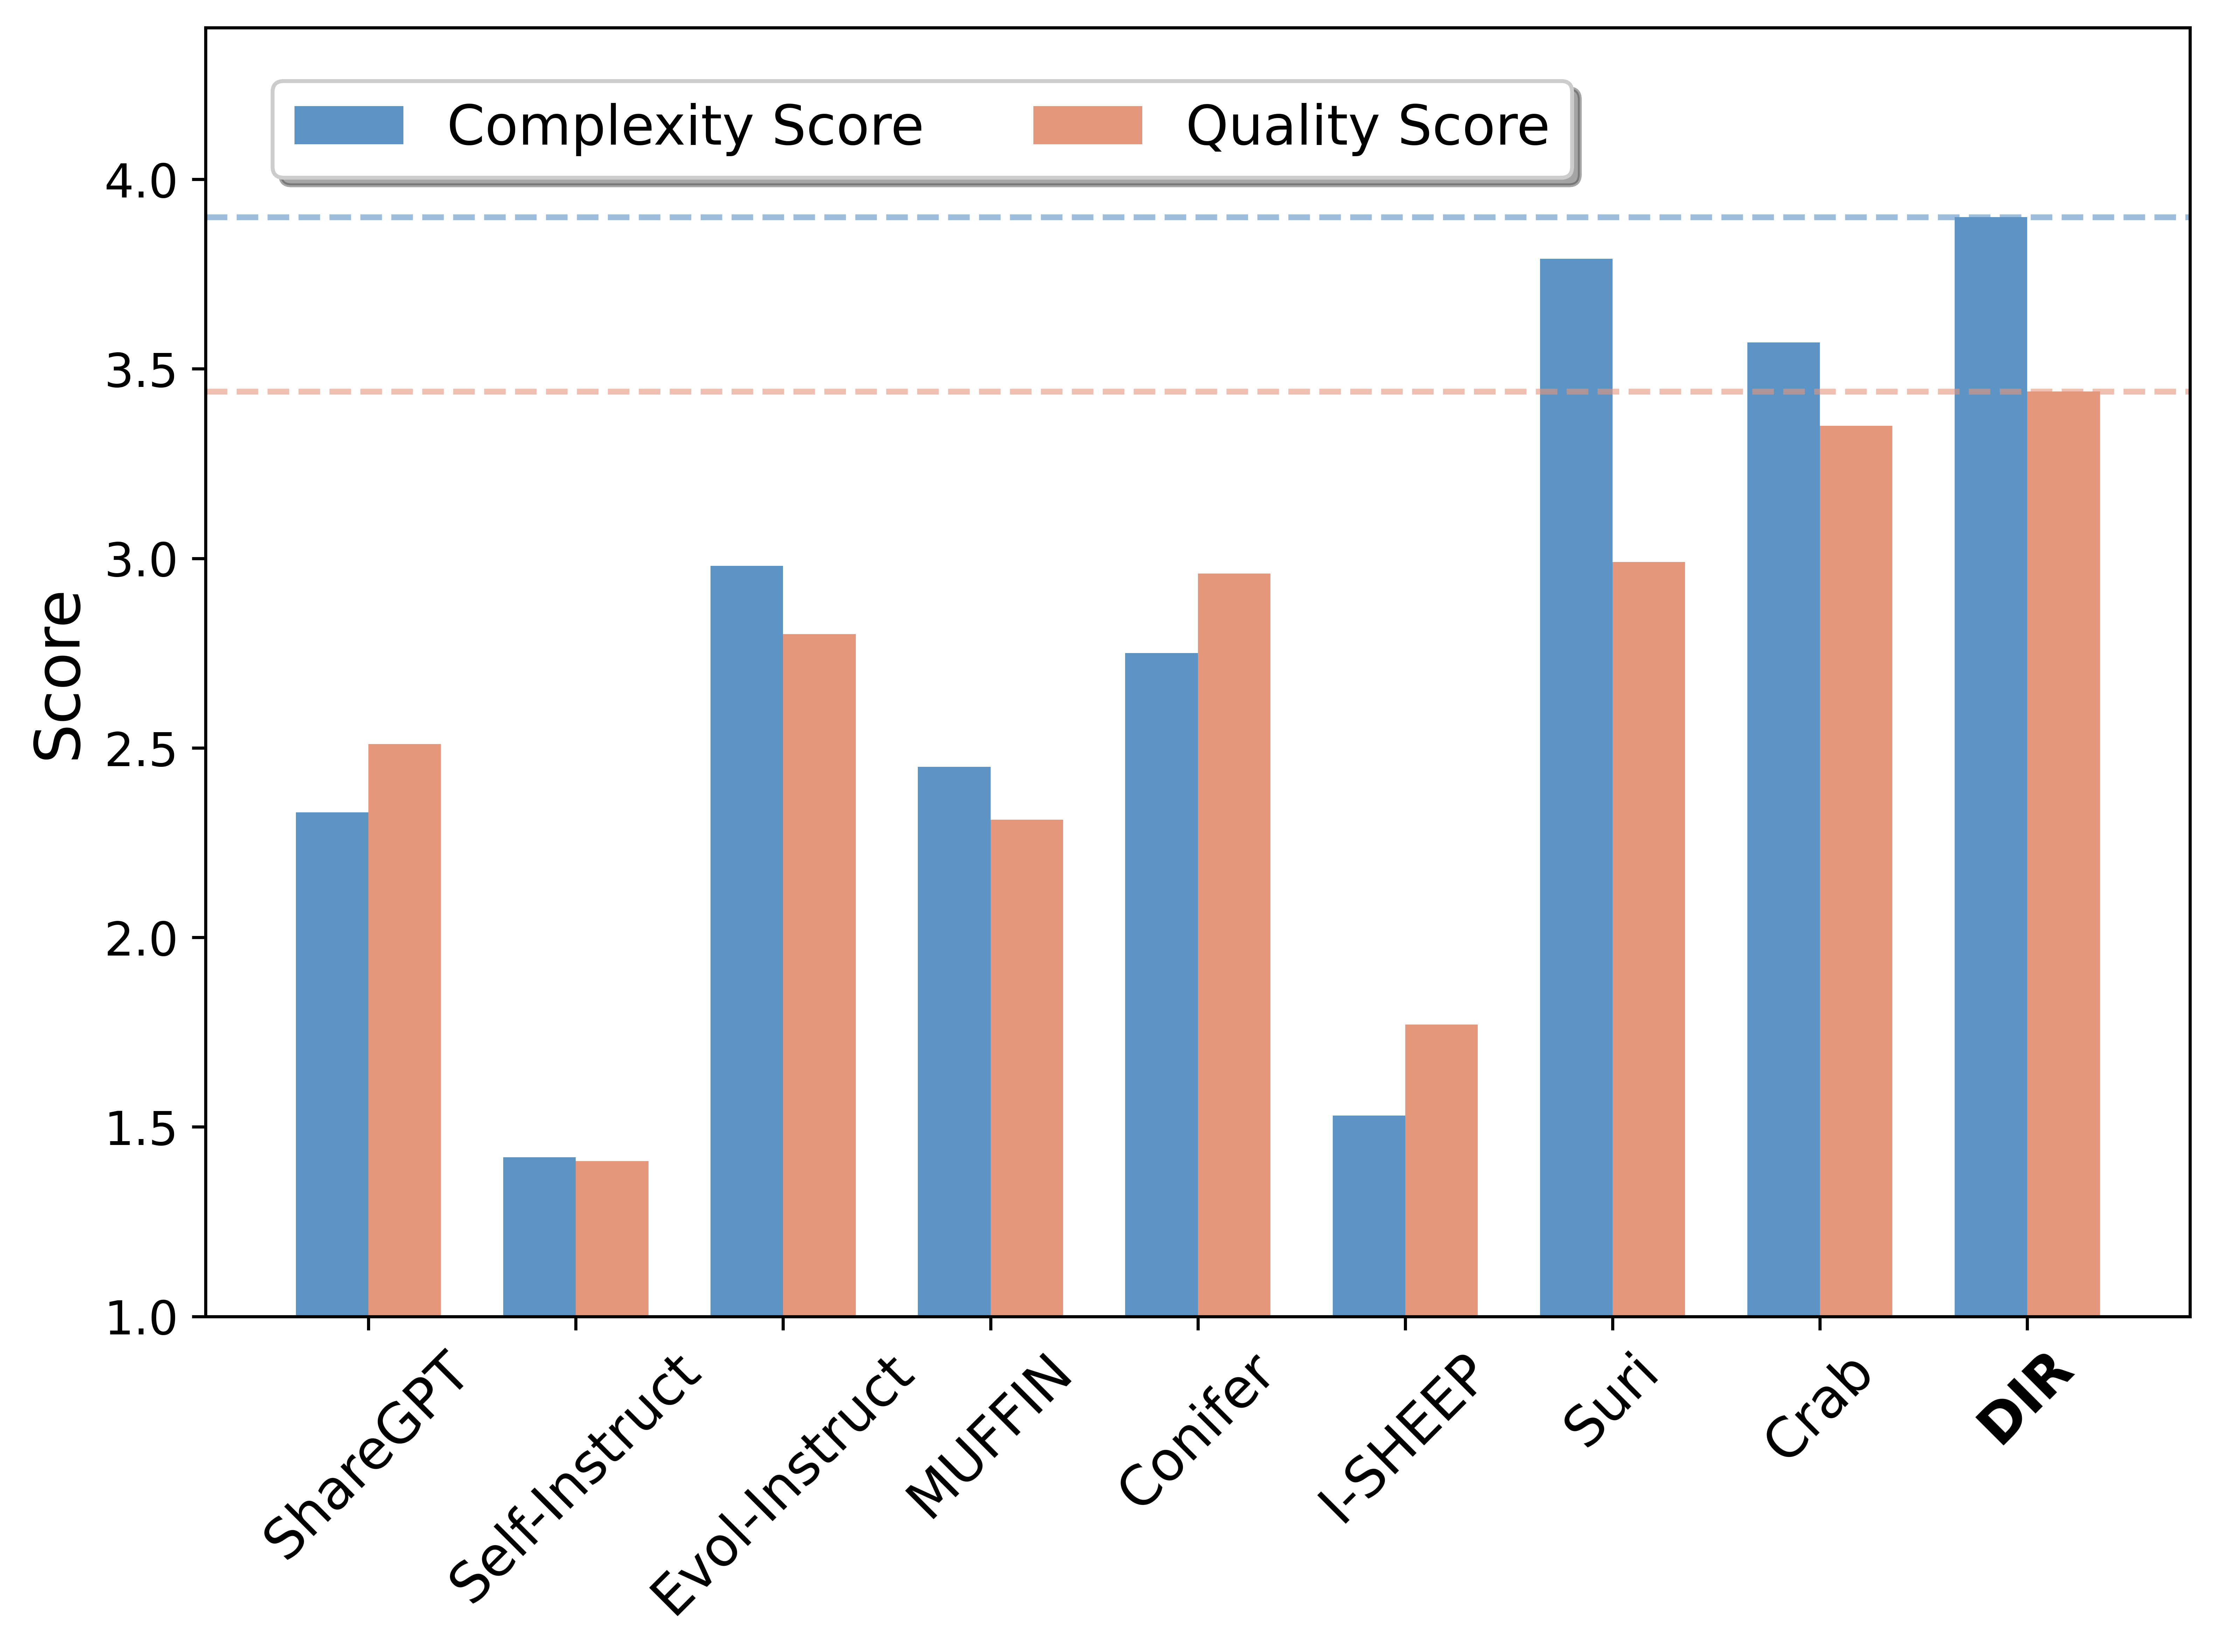
\includegraphics[width=0.9\linewidth]
{source/complexity_scores.png}
\caption{Averaged complexity and quality scores on different datasets.}
\label{figure:complexity_scores}
\end{figure}


% 轮次间的指令长度变化情况，complexity score和quality score变化情况
\begin{figure}[pos=htbp]
\centering
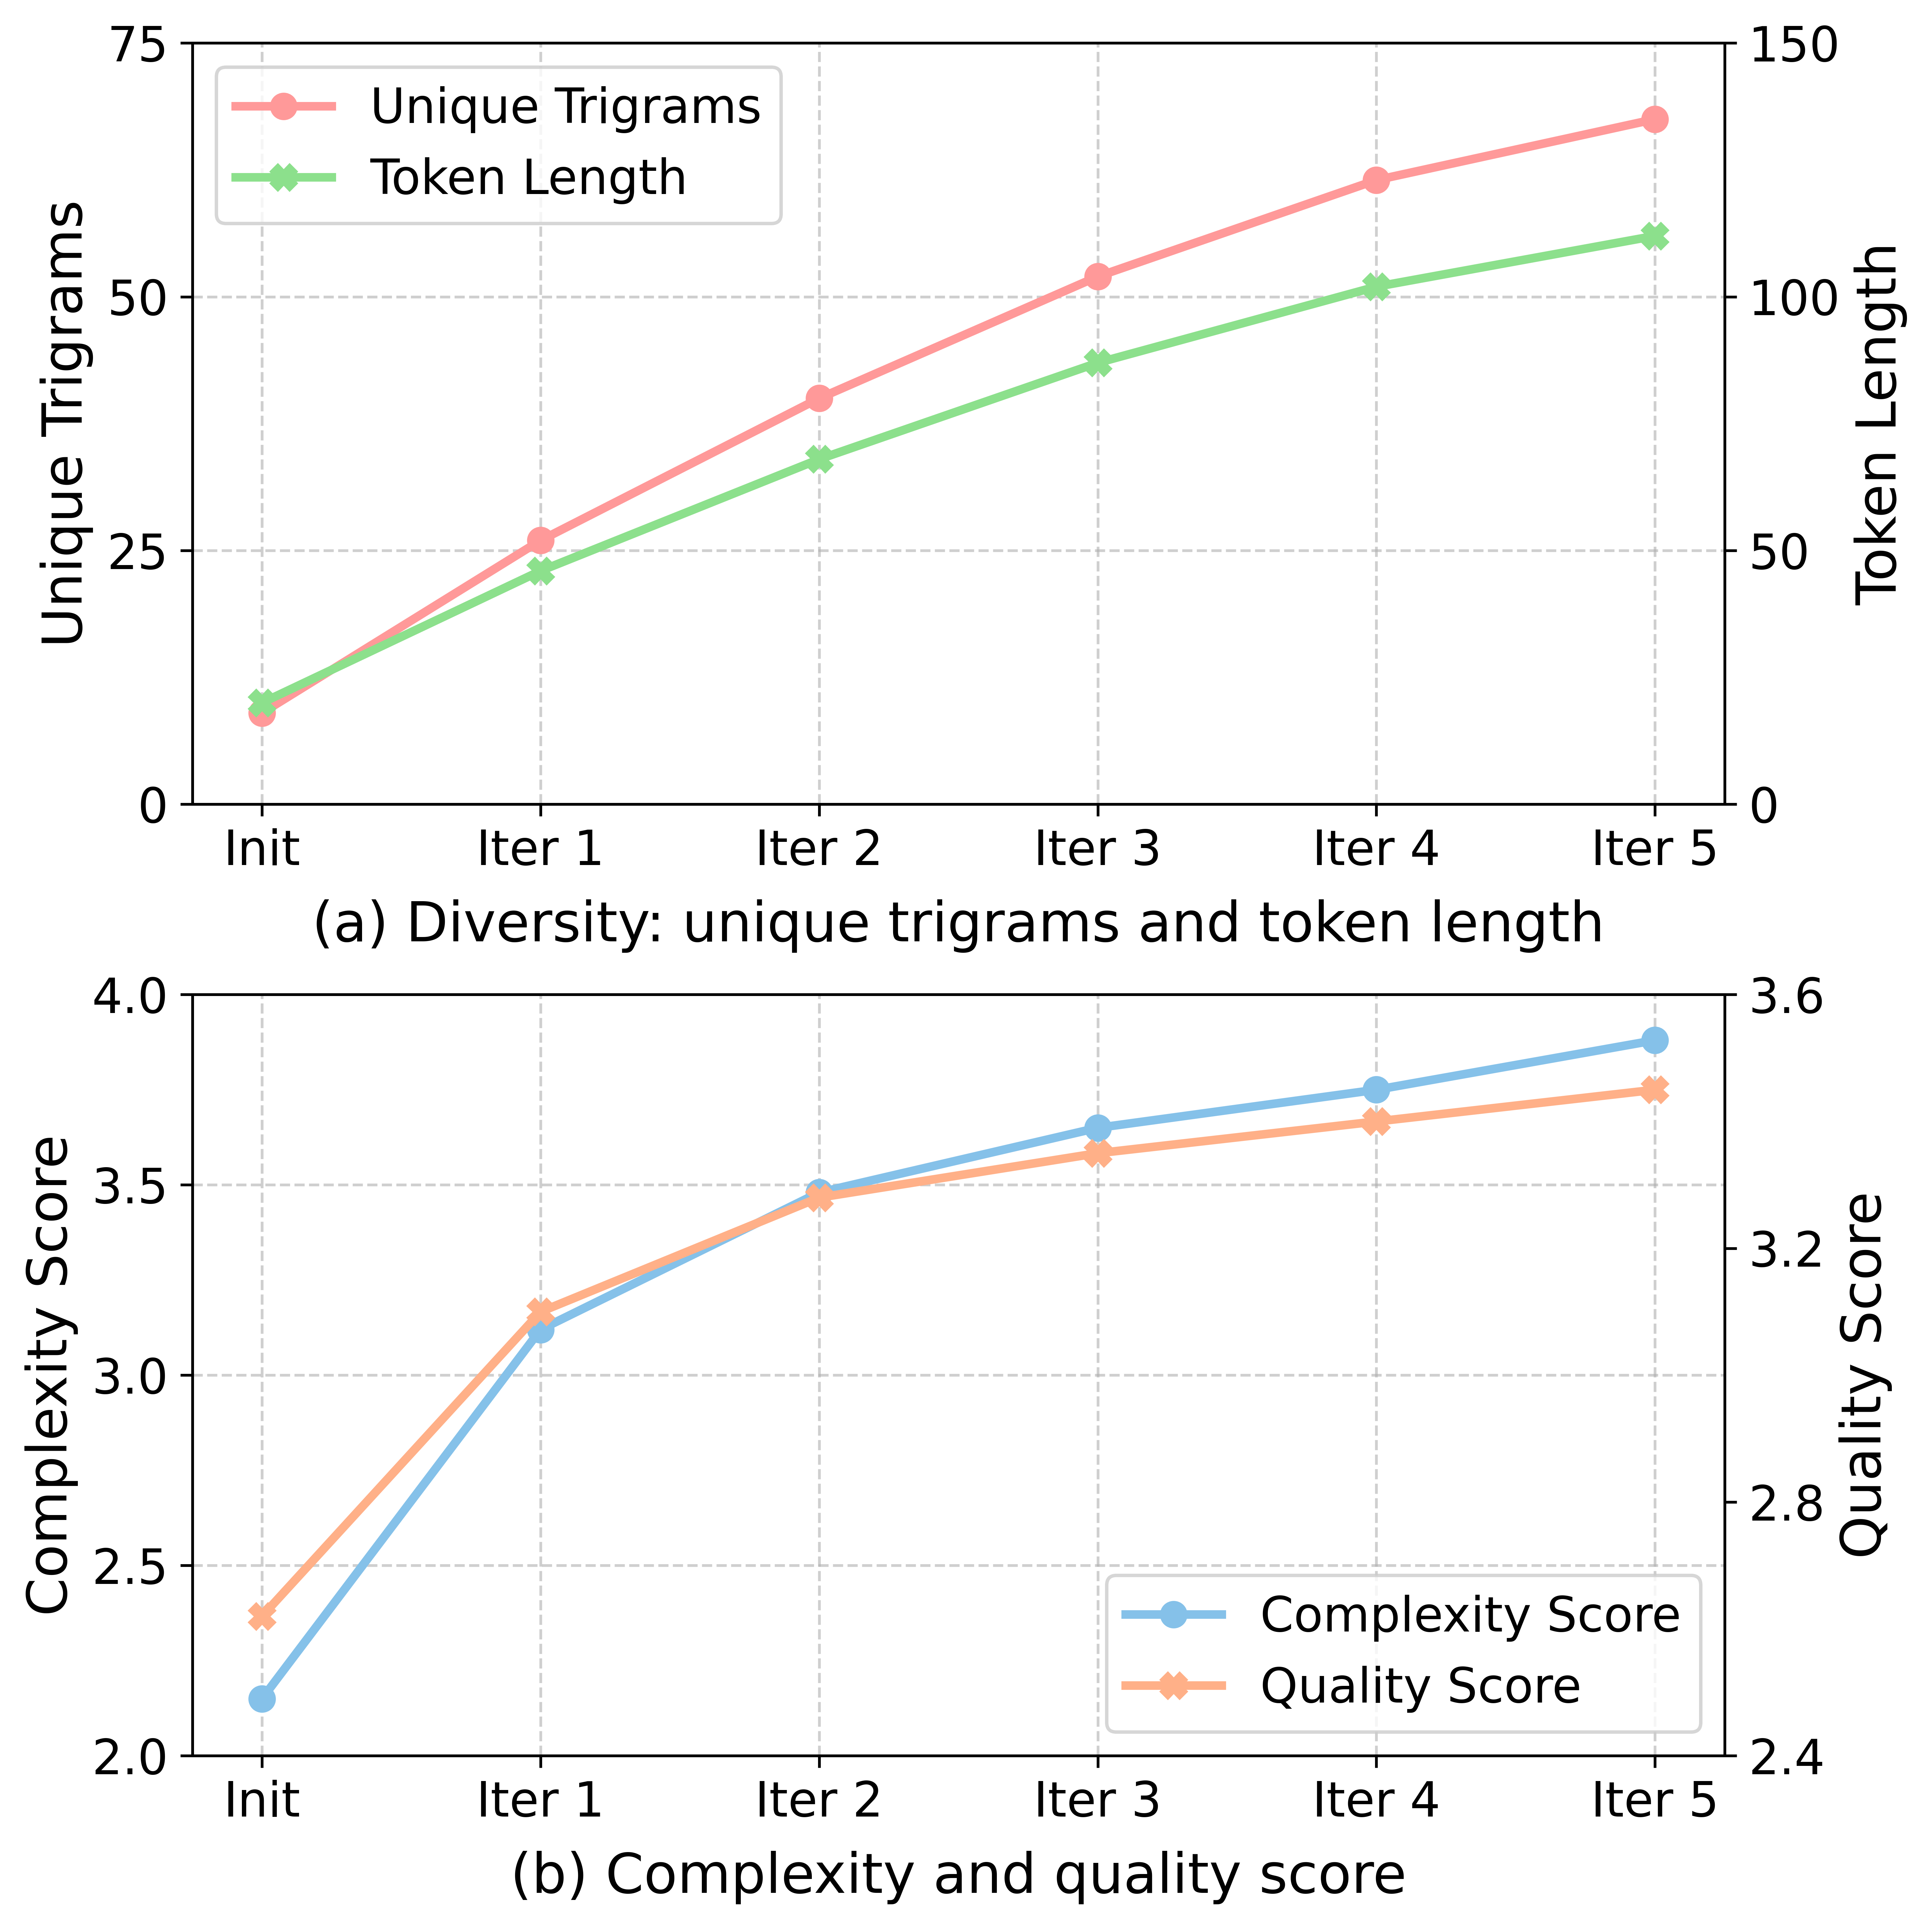
\includegraphics[width=0.95\linewidth]{source/instruction_and_complexity.png}
\caption{Variation of quality indicators of DIR generated data across iterations. \textit{Init} represents initial instructions generated by IIG.}
\label{figure:instruction_and_complexity}
\end{figure}

% To investigate the effect of iterative refinement, we analyze the variation of average unique trigrams and token lengths across iterations in Figure \ref{figure:instruction_and_complexity}(a). The results demonstrate consistent increases in both instruction length and unique trigrams, indicating that newly added constraints are diverse rather than mere repetition. Furthermore, Figure \ref{figure:instruction_and_complexity}(b) displays the evolution of complexity and quality scores throughout the iterations, showing steady improvement of data quality as the iterations progress.

To quantitatively assess data quality, we employed the DEITA scorer \citep{liu2024Deita}, which leverages an LLM-based framework to evaluate instruction complexity and the overall quality of instruction-response pairs. As shown in Figure \ref{figure:complexity_scores}, our approach significantly outperforms previous instruction datasets in terms of both complexity and quality scores. Notably, our method shows marginal improvements over automatic back-translation approaches like Suri and Crab, despite their use of high-quality seed datasets (e.g., Alpaca-GPT4 for Crab) and advanced models (e.g., GPT-4-turbo for Suri). These results validate the effectiveness of our data synthesis strategy.

Furthermore, we investigated the impact of the iterative refinement process by tracking key quality indicators over five iterations (Figure \ref{figure:instruction_and_complexity}). As shown in Figure \ref{figure:instruction_and_complexity}(a), both average token length and the count of unique trigrams exhibit a steady, near-linear increase. This confirms that each iteration introduces novel, non-redundant constraints, thereby enhancing constraint diversity rather than merely repetition. Correspondingly, Figure \ref{figure:instruction_and_complexity}(b) shows that complexity and quality scores improve monotonically. Notably, while the most substantial gains occur in the initial iterations, the continued upward trend across all metrics confirms the efficacy of the iterative cycle in progressively elevating data sophistication.

\subsection{Human Preference Evaluation}

To complement our automated quality evaluation metrics, we conducted a blind, pairwise human evaluation to compare instructions generated by our DIR framework against three representative baselines: \textbf{ShareGPT}, \textbf{Conifer} \citep{sun2024conifer} and \textbf{Crab} \citep{qi2024constraint}. To ensure a fair and controlled comparison, each instruction pair was generated from identical source corpora. From each baseline, 100 samples were randomly selected for side-by-side comparison. Three annotators with Master's degrees and proficiency in NLP were recruited. The annotators were asked to select a winner for each instruction pair based on three evaluation criteria: \textit{Instruction Complexity}, \textit{Instruction Clarity}, and \textit{Overall Preference}. The final results, determined by majority vote, are presented in Table \ref{table:human_eval_results}.

\begin{table}[!t]
\centering
\caption{Pairwise human evaluation for data quality.}
\renewcommand{\arraystretch}{0.95}
\resizebox{0.48\textwidth}{!}{
\begin{tabular}{cl|ccc}
\toprule
\textbf{Comparison} & \textbf{Evaluation Criterion} & \textbf{Win} & \textbf{Lose} & \textbf{Tie} \\
\midrule
\multirow{3}{*}{\makecell[c]{DIR \\ vs. \\ ShareGPT}} & Instruction Complexity & \textbf{66.0} & 30.0 & 4.0 \\
& Instruction Clarity & \textbf{58.0} & 33.0 & 9.0 \\
& Overall Preference & \textbf{60.0} & 29.0 & 11.0 \\
\midrule
\multirow{3}{*}{\makecell[c]{DIR \\ vs. \\ Conifer}} & Instruction Complexity & \textbf{69.0} & 21.0 & 10.0 \\
& Instruction Clarity & \textbf{67.0} & 23.0 & 10.0 \\
& Overall Preference & \textbf{68.0} & 23.0 & 9.0 \\
\midrule
\multirow{3}{*}{\makecell[c]{DIR \\ vs. \\ Crab}} & Instruction Complexity & \textbf{70.0} & 23.0 & 7.0 \\
& Instruction Clarity & \textbf{67.0} & 27.0 & 6.0 \\
& Overall Preference & \textbf{67.0} & 21.0 & 12.0 \\
\bottomrule
\end{tabular}}
\label{table:human_eval_results}
\end{table}

\begin{table}[!t]
\centering
\renewcommand{\arraystretch}{1.0}
\caption{Inter-annotator agreement for pairwise human evaluation.}
\resizebox{0.32\textwidth}{!}{
\begin{tabular}{lc}
\toprule
\textbf{Comparison} & \textbf{Fleiss' Kappa (\%)} \\
\midrule
DIR vs. ShareGPT & 82.82 \\
DIR vs. Conifer  & 83.34 \\
DIR vs. Crab     & 80.47 \\
\bottomrule
\end{tabular}}
\label{table:human_eval_kappa}
\end{table}

As can be seen, the results reveal an overwhelming preference for instructions generated by our DIR framework across all criteria. This study provides human-centric evidence that the instructions generated by DIR are not only more complex but also more aligned with human preference than other instruction synthesis methods. 

To ensure the reliability of these judgments, we also calculated the inter-annotator agreement using Fleiss' Kappa \citep{fleiss1971measuring}. As shown in Table \ref{table:human_eval_kappa}, the high agreement scores confirm the consistency and validity of our human evaluation process.
\section{Ablation Studies}

\subsection{Influence of Iterative Refinement on SFT Performance}

% \begin{table}[t]
% \centering
% \caption{Experiment results and computational costs for Llama-3-8B-Tulu models across multiple iterations.}
% \renewcommand{\arraystretch}{0.95}
% \resizebox{0.48\textwidth}{!}{
% \begin{tabular}{c|cc|cc|cc}
% \toprule
% \multirow{2}{*}{\textbf{Iteration}} & \multicolumn{2}{c|}{\textbf{FollowBench}} & \multicolumn{2}{c|}{\textbf{AlpacaEval2}} & \multicolumn{2}{c} {\textbf{Token Numbers}} 
% \\
% & \textbf{HSR}        & \textbf{SSR}       & \textbf{LC.}      & \textbf{Len} & \textbf{Input} & \textbf{Output} \\ 
% \midrule
% 1    & 49.75   & 64.78    & 21.63  & 1,994  & 1,882 & 1,869  \\
% 2   & 53.82    & 67.55    & 21.01     & 1,829   & 3,351 & 2,562   \\
% 3   & \textbf{54.46}        & 67.54     & 20.69   & 1,722      & 4,844 & 3,275   \\
% 4   & 53.97       & 67.09    & \textbf{22.50}      & 1,672      & 6,361 & 4,008   \\
% 5   & 53.30     & \textbf{67.91}    & 20.78    & 1,599    & 7,902 & 4,761  \\
% \bottomrule
% \end{tabular}}
% \label{table:judge_iterations}
% \end{table}

\begin{figure}[pos=htbp]
    \centering
    \includegraphics[width=0.48\textwidth]{source/SFT_iterations.png}
    % 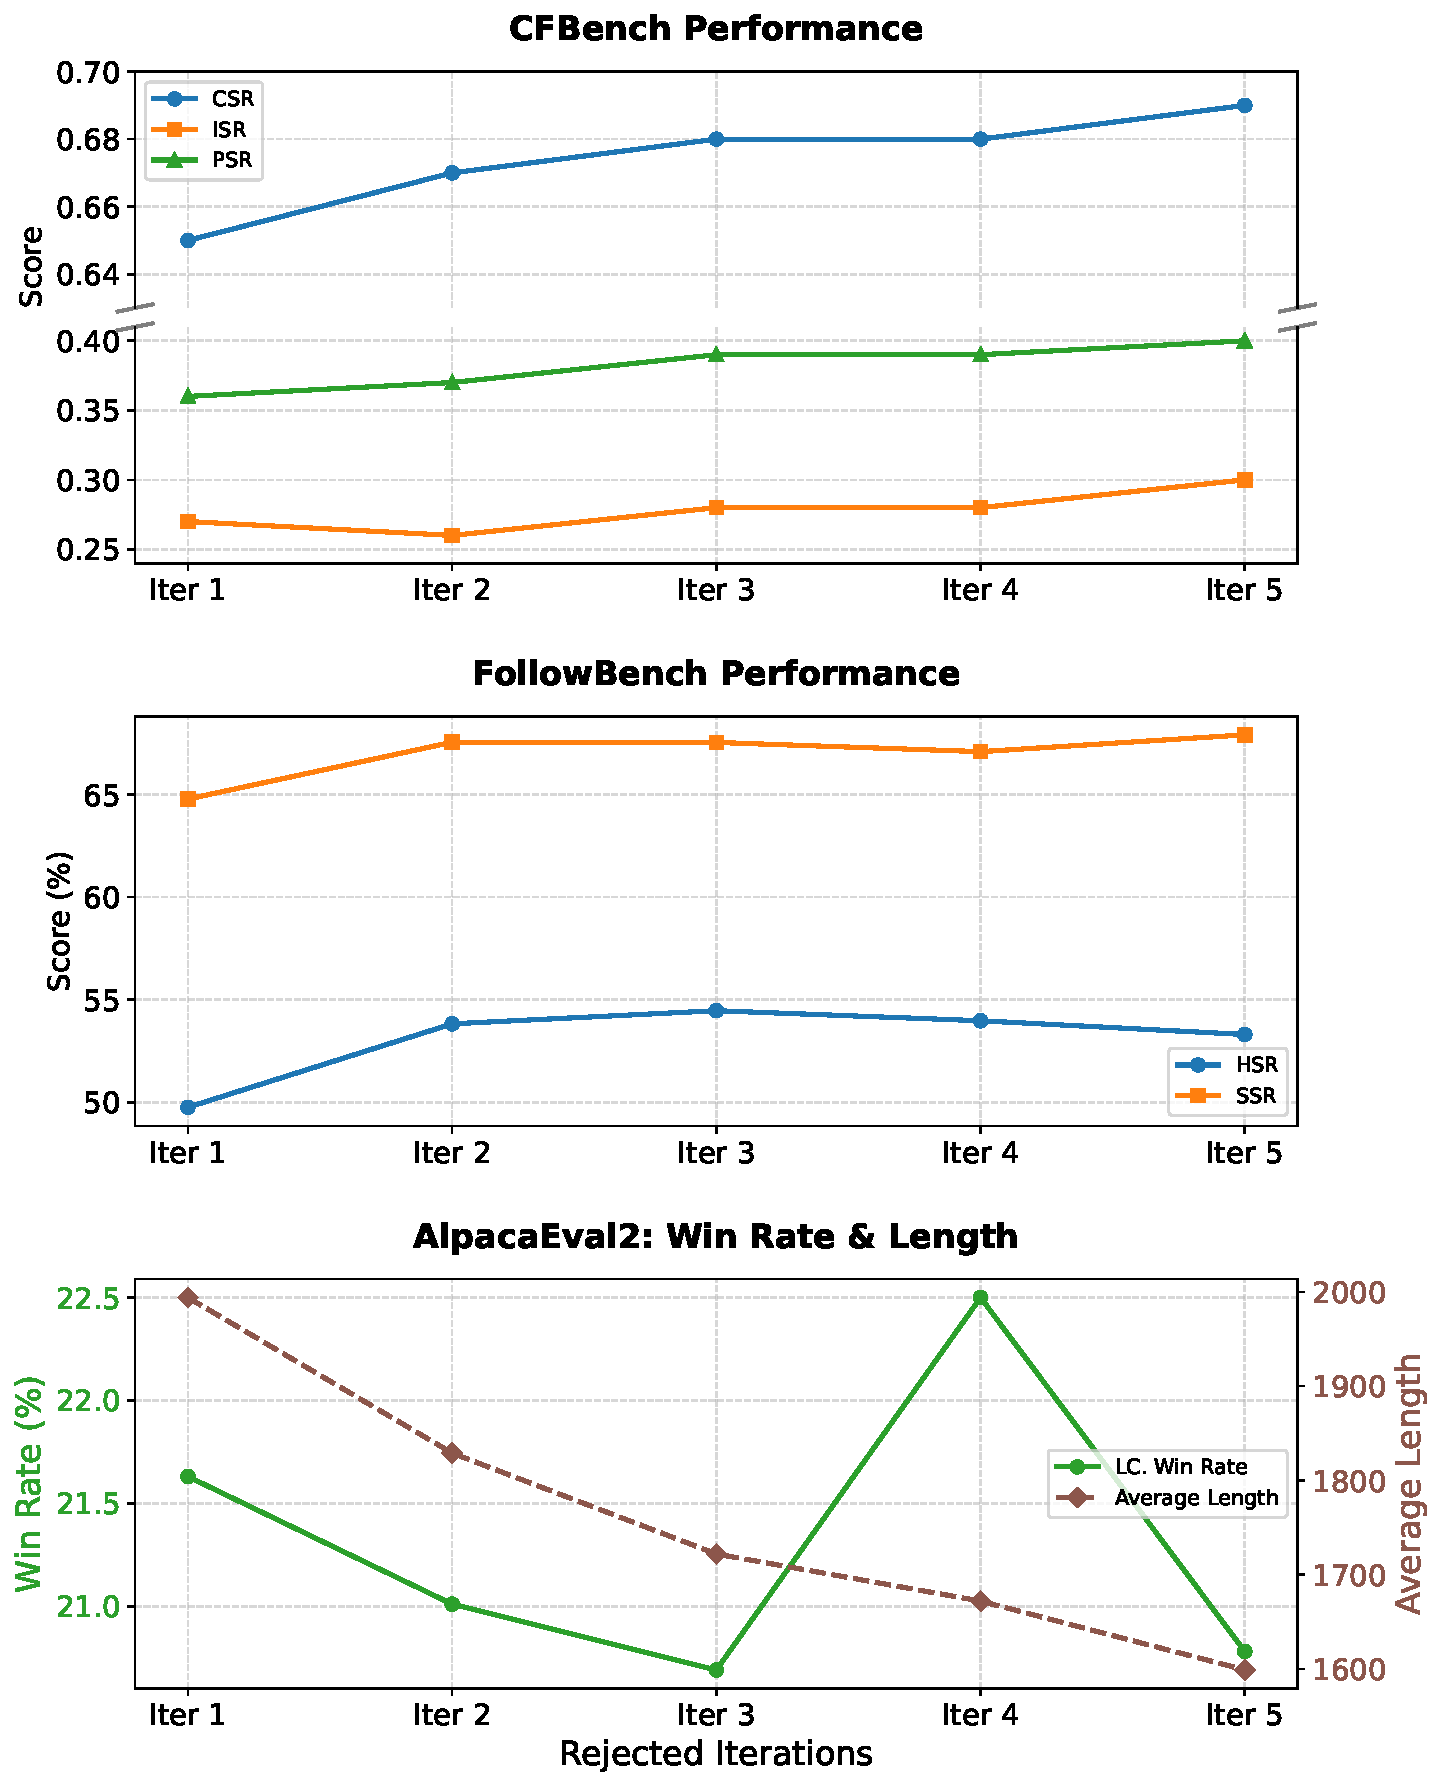
\includegraphics[width=0.48\textwidth]{source/sft_multi_turn.pdf}
    \caption{SFT performance with data from different iterations on Llama-3-8B-Tulu.}
    \label{figure:iterative_sft}
\end{figure}

As discussed in Section \ref{sec:IIR}, we apply multiple refinement iterations to ensure the quality of complex instructions. In this section, we investigate the effectiveness of our iterative refinement approach by measuring SFT model performance across different iterations. As shown in Figure \ref{figure:iterative_sft}, we evaluate SFT models trained on data from different iterations.

% and track the average input and output token counts to quantify the computational cost associated with each iteration.

% 下面这里增加了cfbench结果，画图代码在：source/sft_multi_turn_figure.py

Specifically, we observe consistent improvements on CFBench, FollowBench and AlpacaEval2 through the first two iterations. In particular, CFBench exhibits steady growth across all metrics. This suggests that the iterative judging process effectively identifies and incorporates increasingly sophisticated constraints that are valuable for complex instruction following. However, improvements tend to plateau after the third iteration. This could be attributed to the fact that the most critical and fundamental constraints for effective alignment have already been discovered in earlier iterations. Furthermore, we observe a steady decline in the average output length on AlpacaEval2. This indicates that the iteration process enhances alignment precision, enabling the model to provide more concise responses without unnecessary verbosity.

To verify that the benefits of iterative refinement do not stem simply from an increased number of constraints, we compared our method against a one-shot baseline, where multiple constraints are generated simultaneously without iteration. As shown in Table \ref{table:judge_iterations2}, the one-shot approach is less effective for SFT, as it lacks the progressive discovery process, which is crucial for uncovering challenging constraints with higher complexity (measured by Unique Trigrams).

% We further present computational cost analysis in Figure \ref{figure:instruction_and_complexity}. As can be seen, the metrics demonstrate a steady improvement of data quality as the iterations progress. While multiple iterations introduce additional computational overhead, they are crucial for generating more valuable constraints and improving the model's ability.

% 这个子图已经去掉了
% Moreover, as shown in Figure \ref{figure:instruction_and_complexity}, data quality improves steadily across iterations. Despite the increased computational costs reflected in Figure \ref{figure:iterative_sft}, where both input and output token numbers increase, requiring more computational resources for training, these iterations generate more valuable constraints that directly enhance model performance.

\begin{table}[!t]
\centering
\caption{SFT performance of 1-shot and 5-iteration instruction generation on Llama-3-8B-Tulu.}
\renewcommand{\arraystretch}{0.95}
\resizebox{0.48\textwidth}{!}{
\begin{tabular}{c|cc|cc|c}
\toprule
\multirow{2}{*}{\textbf{Method}} & \multicolumn{2}{c|}{\textbf{FollowBench}} & \multicolumn{2}{c|}{\textbf{AlpacaEval2}} & \multirow{2}{*}{\textbf{Uni-Trigrams}}
\\
& \textbf{HSR}        & \textbf{SSR}       & \textbf{LC.}      & \textbf{Len}  \\ 
\midrule
1-shot   & 50.17     & 63.82    & 18.49    & 1,566 & 41.72 \\
5-iteration	   & \textbf{53.30}     & \textbf{67.91}    & \textbf{20.78}    & 1,599  & 67.45 \\
\bottomrule
\end{tabular}}
\label{table:judge_iterations2}
\end{table}

\subsection{Influence of Iterative Refinement on RM Efficacy}

\begin{table*}[!t]
\centering
\caption{SFT performance with constraints from different judgment strategies on Llama-3-8B models (UltraChat and Tulu).}
\renewcommand{\arraystretch}{1.1}
\resizebox{0.85\textwidth}{!}{
\begin{tabular}{l|l|ccc|cc|cc}
\toprule
\multirow{2}{*}{\textbf{Base Model}} & \multirow{2}{*}{\textbf{Method}} & \multicolumn{3}{c}{\textbf{CF-Bench}} & \multicolumn{2}{c}{\textbf{FollowBench}} & \multicolumn{2}{c}{\textbf{AlpacaEval2}} \\
\cmidrule(lr){3-5} \cmidrule(lr){6-7} \cmidrule(lr){8-9}
& & \textbf{CSR} & \textbf{ISR} & \textbf{PSR} & \textbf{HSR} & \textbf{SSR} & \textbf{LC.} & \textbf{Len} \\
\midrule
\multirow{5}{*}{\makecell[l]{Llama-3-8B-UltraChat}} 
& Baseline & 0.51 & 0.15 & 0.22 & 41.04 & 57.39 & 8.86 & 1,017 \\
\cmidrule{2-9} % <--- 为 UltraChat 部分添加横线
& No Judge & 0.63 & 0.25 & 0.34 & 47.15 & 62.62 & 19.07 & 1,706 \\
& Document-free Judge & 0.62 & 0.25 & 0.34 & 51.24 & 63.81 & 20.00 & 1,717 \\
& \textbf{Document-based Judge} & \textbf{0.64} & \textbf{0.26} & \textbf{0.34} & \textbf{52.34} & \textbf{64.09} & 19.74 & 1,408 \\
& \quad + check & 0.61 & 0.24 & 0.31 & 50.69 & 63.89 & \textbf{21.00} & 1,813 \\
\midrule
\midrule
\multirow{5}{*}{\makecell[l]{Llama-3-8B-Tulu}} 
& Baseline & 0.50 & 0.15 & 0.20 & 34.91 & 51.76 & 5.20 & 995 \\
\cmidrule{2-9} % <--- 为 Tulu 部分添加横线
& No Judge & 0.66 & 0.28 & 0.38 & 47.59 & 63.60 & 18.32 & 2,067 \\
& Document-free Judge & 0.67 & 0.27 & 0.38 & 50.62 & 63.69 & 17.02 & 2,842 \\
& \textbf{Document-based Judge} & \textbf{0.67} & \textbf{0.27} & \textbf{0.38} & \textbf{54.16} & \textbf{67.52} & 20.45 & 1,639 \\
& \quad + check & 0.66 & 0.26 & 0.37 & 51.35 & 66.09 & \textbf{21.09} & 2,049 \\
\bottomrule
\end{tabular}}
\label{table:judge}
\end{table*}

\begin{figure}[pos=htbp]
    \centering
    \includegraphics[width=0.48\textwidth]{source/RM_iterations.png}
    \caption{RL performance with RM trained on rejected responses from different iterations on Llama-3-8B-UltraChat.}
    \label{figure:iterative_rm}
\end{figure}

As discussed in Section \ref{sec:rl}, we utilize responses generated from different iterations as rejected samples for RM training. To investigate how the gap between chosen and rejected samples influences RM efficacy, we trained multiple RMs by pairing a fixed set of chosen samples with rejected samples from varying iterations. These RMs were subsequently employed in RL training to evaluate their impact on alignment performance, as shown in Figure \ref{figure:iterative_rm}.

The results show that RL performance follows an inverted U-shaped trend as the iteration index of rejected samples increases. Utilizing responses from the second iteration as rejected samples yielded optimal performance across both complex and general benchmarks. Notably, the average output length on AlpacaEval2 decreased significantly with Iter 2, indicating that the model effectively suppressed verbosity while improving overall performance.

Using rejected samples from either too early or too late iterations leads to performance degradation. With later iterations (e.g., Iter 4-5), the quality of rejected samples improves to the point where they closely resemble chosen responses, narrowing the contrastive space and hindering the RM's ability to capture preference signals. Conversely, with earlier iterations (e.g., Iter 0-1), the gap between chosen and rejected samples is so large that the task becomes trivial, preventing the RM from learning to distinguish fine-grained quality differences. In summary, selecting rejected samples of moderate difficulty is crucial for ensuring RM's efficacy for the RL process.

\subsection{Judgment Strategy for Better Constraint}
\label{sec:judge}

% \begin{table}[!t]
% \centering
% \caption{Experiment results on Llama-3-8B models with constraints from different judgment strategies.}
% \renewcommand{\arraystretch}{0.95}
% \resizebox{0.44\textwidth}{!}{
% \begin{tabular}{c|cc|cc}
% \toprule
% \multirow{2}{*}{\textbf{Method}} & \multicolumn{2}{c|}{\textbf{FollowBench}} & \multicolumn{2}{c}{\textbf{AlpacaEval2}} \\
% & \textbf{HSR} & \textbf{SSR} & \textbf{LC.} & \textbf{Len} \\
% \midrule
% \multicolumn{5}{l}{\textit{Results on Llama-3-8B-UltraChat}} \\
% \midrule
% Baseline & 41.04 & 57.39 & 8.86 & 1,017 \\
% \midrule
% w/o judge & 47.15 & 62.62 & 19.07 & 1,706 \\
% judge w/o doc & 51.24 & 63.81 & 20.00 & 1,717 \\
% judge w/ doc & \textbf{52.34} & \textbf{64.09} & 19.74 & 1,408 \\
% \midrule
% w/ check & 50.69 & 63.89 & \textbf{21.00} & 1,813 \\
% \midrule
% \multicolumn{5}{l}{\textit{Results on Llama-3-8B-Tulu}} \\
% \midrule
% Baseline & 34.91 & 51.76 & 5.20 & 995 \\
% \midrule	
% w/o judge & 47.59 & 63.60 & 18.32 & 2,067 \\
% judge w/o doc & 50.62 & 63.69 & 17.02 & 2,842 \\
% judge w/ doc & \textbf{54.16} & \textbf{67.52} & 20.45 & 1,639 \\
% \midrule
% w/ check & 51.35 & 66.09 & \textbf{21.09} & 2,049 \\
% \bottomrule
% \end{tabular}}
% \label{table:judge}
% \end{table}

\begin{table}[!t]
\centering
\caption{SFT performance with different sampling strategies on Llama-3-8B-UltraChat .}
\renewcommand{\arraystretch}{0.95}
\resizebox{0.47\textwidth}{!}{
\begin{tabular}{c|cc|cc|c}
\toprule
\multirow{2}{*}{\textbf{Method}} & \multicolumn{2}{c|}{\textbf{FollowBench}} & \multicolumn{2}{c|}{\textbf{AlpacaEval2}} & \textbf{Unique} \\
& \textbf{HSR}        & \textbf{SSR}       & \textbf{LC.}      & \textbf{Len} & \textbf{Trigrams} \\ 
\midrule
Baseline  & 41.04       & 57.39      & 8.86       & 1,017 & - \\
\midrule
Random 1K    & 41.71   & 57.66    & 12.26  & 1,313 & 45.13 \\
Density 1K    & \textbf{45.85}   & \textbf{60.21}    & \textbf{17.15}  & 1,611 & \textbf{66.81} \\
InsTag 1K   & 44.11    & 59.89    & 13.03     & 1,251 & 58.09 \\
\bottomrule
\end{tabular}}
\label{table:sampling}
\end{table}

In this section, we investigate the optimal judgment strategy for constraint generation by comparing three distinct configurations: (1) No Judgment, where constraints are generated directly; (2) Document-free Judgment, which relies on the guidance model’s own response as the basis for new constraints; and (3) Document-based Judgment, which leverages the refined document as the reference for new constraints.

As shown in Table \ref{table:judge}, the iterative judgment process is indispensable for uncovering valuable constraints that enhance instruction-following capabilities. Notably, the Document-based Judgment setting achieves the best performance on both complex and general instruction benchmarks. This suggests that the refined document serves as a crucial gold standard, allowing the LLM-judge to pinpoint model deficiencies more accurately than when relying on self-generated, potentially flawed outputs. This mechanism mirrors human behavior: when users refine prompts based on model outputs, they typically hold an intrinsic reference in mind and issue constraints to guide the response toward that expectation.

Regarding the additional checking step (+ check), where generated constraints are further filtered based on their alignment with the model's eventual output, we observe a decline in complex instruction-following performance. This suggests that the checking mechanism may be overly restrictive, inadvertently filtering out subtle yet essential constraints that are necessary for precise instruction alignment. 

% However, this step improves performance on general instruction following on AlpacaEval2, revealing a trade-off: stricter constraint filtering favors general conversational fluency but is harmful for complex instruction adherence.

\begin{figure}[pos=htbp]
\centering
\includegraphics[width=0.48\textwidth]{source/llama_Tulu_DataNum.png}
\caption{SFT performance with different data volume on Llama-3-8B-Tulu.}
\label{figure:data_num}
\end{figure}

\begin{table*}[!t]
\centering
\caption{RL performance with different RM configurations on Llama-3-8B-UltraChat and Qwen-2.5-7B-UltraChat.}
% \setlength{\tabcolsep}{8pt}
\renewcommand{\arraystretch}{1.1}
\resizebox{0.85\textwidth}{!}{
\begin{tabular}{l|l|ccc|cc|cc}
\toprule
\multirow{2}{*}{\textbf{Base Model}} & \multirow{2}{*}{\textbf{Method}} & \multicolumn{3}{c}{\textbf{CF-Bench}} & \multicolumn{2}{c}{\textbf{FollowBench}} & \multicolumn{2}{c}{\textbf{AlpacaEval2}} \\
\cmidrule(lr){3-5} \cmidrule(lr){6-7} \cmidrule(lr){8-9}
& & \textbf{CSR} & \textbf{ISR} & \textbf{PSR} & \textbf{HSR} & \textbf{SSR} & \textbf{LC.} & \textbf{Len} \\
\midrule
\multirow{5}{*}{\makecell[l]{Llama-3-8B-UltraChat}} 
& Baseline & 0.51 & 0.15 & 0.22 & 41.04 & 57.39 & 8.86 & 1,017 \\
\cmidrule{2-9}
& DIR-SFT & 0.61 & 0.24 & 0.31 & 50.69 & 63.89 & 21.00 & 1,813 \\
& DIR-RL w/ RM-3B & 0.62 & 0.24 & 0.32 & 51.31 & 64.03 & 21.89 & 2,387 \\
& \textbf{DIR-RL w/ RM-8B} & \textbf{0.62} & \textbf{0.26} & \textbf{0.34} & \textbf{53.83} & \textbf{65.55} & \textbf{22.07} & 2,271 \\
& \quad w/o Rule-based Reward & 0.60 & 0.24 & 0.32 & 52.17 & 63.82 & 20.91 & 2,413 \\
\midrule
\midrule
\multirow{5}{*}{\makecell[l]{Qwen-2.5-7B-UltraChat}} 
& Baseline & 0.68 & 0.29 & 0.40 & 47.71 & 64.79 & 10.87 & 836 \\
\cmidrule{2-9}
& DIR-SFT & 0.76 & 0.41 & 0.51 & 59.07 & 71.35 & 32.43 & 1,779 \\
& DIR-RL w/ RM-3B & 0.76 & 0.43 & 0.53 & 60.04 & 72.57 & 33.00 & 2,109 \\
& \textbf{DIR-RL w/ RM-8B} & \textbf{0.77} & \textbf{0.45} & \textbf{0.54} & \textbf{62.53} & \textbf{72.68} & \textbf{35.49} & 1,988 \\
& \quad w/o Rule-based Reward & 0.74 & 0.42 & 0.51 & 59.94 & 70.10 & 32.88 & 2,179 \\
\bottomrule
\end{tabular}}
\label{table:rm-training}
\end{table*}

\subsection{Impact of SFT Configurations}

In this section, we investigate the impact of various SFT configurations on DIR's performance, focusing primarily on two key factors: the sampling strategy for document selection and the volume of training data.

As detailed in Section \ref{sec:document_collection}, we utilize density-based sampling to ensure the diversity of our document set. To verify the effectiveness of this approach, we compared it against two baselines for selecting SFT samples:

\begin{enumerate}[itemsep=1mm, parsep=0pt, leftmargin=*]
    \item \textbf{Random 1K}: Randomly selecting 1K samples.
    \item \textbf{Density 1K}: Selecting 1K samples using our proposed density-based sampling method.
    \item \textbf{InsTag 1K} \citep{Lu2023InsTagIT}: Using GPT-4\footnote{Specifically, we use GPT-4o-0806 for InsTag.} to label each instruction with semantic and complexity tags, then selecting instructions to ensure diverse representation.
\end{enumerate}

As shown in Table \ref{table:sampling}, our density-based method significantly outperforms both random selection and InsTag across complex and general instruction-following benchmarks. Notably, despite the high computational cost associated with InsTag's LLM-based tagging process, InsTag yields lower performance than our approach. We also analyzed the lexical diversity of the sampled instructions by calculating the average unique trigrams. The results indicate that our method selects more diverse samples (66.81 unique trigrams), which correlates with the superior downstream performance.

We further analyze the relationship between training data volume and SFT performance in Figure \ref{figure:data_num}. As can be seen, performance on both general and complex instruction benchmarks scales positively with the amount of training data, underscoring the scalability of the DIR framework. On the other hand, the model can achieve superior performance with only 1K training samples, highlighting the efficiency of our data synthesis process in minimizing SFT overhead.

\subsection{Impact of RM Configurations}

To investigate the impact of RM configurations on downstream RL performance, we conduct ablation studies on model scale and the integration of rule-based reward signals. Table \ref{table:rm-training} presents a comparative analysis between RMs initialized from Llama-3.2-3B and Llama-3.1-8B, evaluating their effectiveness with and without rule-based components.

Our results demonstrate a positive correlation between RM scale and feedback quality. Across RL experiments on different policy models, the 8B-scale RM consistently outperforms its 3B counterpart. This performance gap likely stems from the superior linguistic nuances and logical reasoning inherent in larger base models, allowing the 8B RM to capture more sophisticated preference signals to guide policy optimization.

Furthermore, incorporating rule-based reward signals proved essential, and removing these signals led to a marked performance decline across both complex and general instruction benchmarks. For instruction alignment, verifiable constraints (e.g., formatting, keywords) provide deterministic, low-noise feedback. By establishing a rigid correspondence between constraints and outputs, these signals significantly accelerate convergence during constraint-aware RL.

% \begin{table*}[!ht]
% \centering
% \caption{Experiment results on Llama-3-8B and Qwen-2.5-7B, with both models fine-tuned with ultrachat-200k. Llama-3-70B-Instruct and Qwen-2.5-72B-Instruct are used as the guidance models respectively.}
% \setlength{\tabcolsep}{12pt}
% \renewcommand{\arraystretch}{0.9}
% \resizebox{0.98\textwidth}{!}{
% \begin{tabular}{l|ccc|cc|cc}
% \toprule
% \multicolumn{8}{c}{\textbf{Fine-tuned on Llama-3-8B-UltraChat}} \\
% \midrule
% \multirow{2}{*}{\textbf{Method}} & \multicolumn{3}{c}{\textbf{CFBench}} & \multicolumn{2}{c}{\textbf{FollowBench}} & \multicolumn{2}{c}{\textbf{AlpacaEval2}} \\
% \cmidrule(lr){2-4} \cmidrule(lr){5-6} \cmidrule(lr){7-8}
% & \textbf{CSR} & \textbf{ISR} & \textbf{PSR} & \textbf{HSR} & \textbf{SSR} & \textbf{LC.} & \textbf{Len} \\
% \midrule
% Baseline & 0.51 & 0.15 & 0.22 & 41.04 & 57.39 & 8.86 & 1,017 \\
% DIR-SFT & 0.61 & 0.24 & 0.31 & 50.69 & 63.89 & 21.00 & 1,813 \\
% DIR-RL w/ RM-3B & 0.62 & 0.24 & 0.32 & 51.31 & 64.03 & 21.89 & 2,387 \\
% DIR-RL w/ RM-8B & 0.62 & 0.26 & 0.34 & 53.83 & 65.55 & 22.07 & 2,271 \\
% w/o Rule-based Reward & 0.60 & 0.24 & 0.32 & 52.17 & 63.82 & 20.91 & 2,413 \\
% \midrule
% \midrule
% \multicolumn{8}{c}{\textbf{Fine-tuned on Qwen-2.5-7B-UltraChat}} \\
% \midrule
% \multirow{2}{*}{\textbf{Method}} & \multicolumn{3}{c}{\textbf{CFBench}} & \multicolumn{2}{c}{\textbf{FollowBench}} & \multicolumn{2}{c}{\textbf{AlpacaEval2}} \\
% \cmidrule(lr){2-4} \cmidrule(lr){5-6} \cmidrule(lr){7-8}
% & \textbf{CSR} & \textbf{ISR} & \textbf{PSR} & \textbf{HSR} & \textbf{SSR} & \textbf{LC.} & \textbf{Len} \\
% \midrule
% Baseline & 0.68 & 0.29 & 0.40 & 47.71 & 64.79 & 10.87 & 836 \\
% DIR-SFT & 0.76 & 0.41 & 0.51 & 59.07 & 71.35 & 32.43 & 1,779 \\
% DIR-RL w/ RM-3B & 0.76 & 0.43 & 0.53 & 60.04 & 72.57 & 33.00 & 2,109 \\
% DIR-RL w/ RM-8B & 0.77 & 0.45 & 0.54 & 62.53 & 72.68 & 35.49 & 1,988 \\
% w/o Rule-based Reward & 0.74 & 0.42 & 0.51 & 59.94 & 70.10 & 32.88 & 2,179 \\
% \bottomrule
% \end{tabular}}
% \label{table:rm-training}
% \end{table*}

% \begin{table*}[!ht]
% \centering
% \caption{Main results on Llama-3-8B-UltraChat. We evaluate the performance across CF-Bench, FollowBench, and AlpacaEval2. The best results are highlighted in bold.}
% \setlength{\tabcolsep}{12pt}
% \renewcommand{\arraystretch}{0.9}
% \resizebox{0.98\textwidth}{!}{
% \begin{tabular}{l|ccc|cc|cc}
% \toprule
% \multicolumn{8}{c}{\multirow{2}{*}{\raisebox{1.4em}{\makecell{\textbf{Fine-tuned on Llama-3-8B-UltraChat}}}}} \\
% \midrule
% \multirow{2}{*}{\raisebox{-0.4em}{\textbf{Method}}} & \multicolumn{3}{c}{\textbf{CF-Bench}}      & \multicolumn{2}{c}{\textbf{FollowBench}} & \multicolumn{2}{c}{\textbf{AlpacaEval2}} \\
% \cmidrule(lr){2-4} \cmidrule(lr){5-6} \cmidrule(lr){7-8}
% & \textbf{CSR} & \textbf{ISR} & \textbf{PSR} & \textbf{HSR}        & \textbf{SSR}       & \textbf{LC.}        & \textbf{Len}        \\
% \midrule
% Baseline    & 0.51         & 0.15         & 0.22         & 41.04               & 57.39              & 8.86                & 1,017               \\ 
% \midrule
% DIR-SFT     & 0.61         & 0.24         & 0.31         & 50.69               & 63.89              & 21.00               & 1,813               \\
% \textbf{GRPO (Ours)} & \textbf{0.62} & \textbf{0.26} & \textbf{0.34} & \textbf{53.83}      & \textbf{65.55}     & \textbf{22.07}      & 2,271               \\
% \quad w/o KL Removal & 0.61         & 0.25         & 0.33         & 53.15               & 65.09              & 21.84               & 2,143               \\
% \quad w/o Dynamic Sampling & 0.61         & 0.25         & 0.32         & 52.47               & 64.66              & 21.52               & 2,118               \\
% \midrule
% PPO         & 0.59         & 0.24         & 0.31         & 53.02               & 64.84              & 21.95               & 1,945               \\
% Reinforce++ & 0.59         & 0.23         & 0.31         & 51.96               & 63.71              & 20.88               & 2,629               \\
% \bottomrule
% \end{tabular}}
% \label{table:ablation_no_green}
% \end{table*}

\begin{table*}[!t]
\centering
\caption{Experiment results of different RL methods with RM-8B on Llama-3-8B-UltraChat.}
\renewcommand{\arraystretch}{1.1}
\resizebox{0.85\textwidth}{!}{
\begin{tabular}{l|l|ccc|cc|cc}
\toprule
\multirow{2}{*}{\textbf{Base Model}} & \multirow{2}{*}{\textbf{Method}} & \multicolumn{3}{c}{\textbf{CF-Bench}}      & \multicolumn{2}{c}{\textbf{FollowBench}} & \multicolumn{2}{c}{\textbf{AlpacaEval2}} \\
\cmidrule(lr){3-5} \cmidrule(lr){6-7} \cmidrule(lr){8-9}
& & \textbf{CSR} & \textbf{ISR} & \textbf{PSR} & \textbf{HSR}        & \textbf{SSR}       & \textbf{LC.}        & \textbf{Len}        \\
\midrule
\multirow{7}{*}{\makecell[l]{Llama-3-8B-UltraChat}} 
& Baseline    & 0.51         & 0.15         & 0.22         & 41.04               & 57.39              & 8.86                & 1,017               \\ 
\cmidrule(lr){2-9}
& DIR-SFT     & 0.61         & 0.24         & 0.31         & 50.69               & 63.89              & 21.00               & 1,813               \\
& \textbf{DIR-RL (GRPO)} & \textbf{0.62} & \textbf{0.26} & \textbf{0.34} & \textbf{53.83}      & \textbf{65.55}     & \textbf{22.07}      & 2,271               \\
& \quad w/o KL Relaxation & 0.61         & 0.25         & 0.33         & 53.15               & 65.09              & 21.84               & 2,143               \\
& \quad w/o Dynamic Sampling & 0.61         & 0.25         & 0.32         & 52.47               & 64.66              & 21.52               & 2,118               \\
\cmidrule(lr){2-9}
& PPO         & 0.59         & 0.24         & 0.31         & 53.02               & 64.84              & 21.95               & 1,945               \\
% Reinforce++重训了一遍
& Reinforce++ & 0.61   & 0.25 & 0.33  & 53.54 & 65.26  & 21.76 & 2,403   \\
\bottomrule
\end{tabular}}
\label{table:ablation_rl}
\end{table*}

\subsection{Influence of RL Settings}

During the RL training phase, we implemented two key enhancements to the standard GRPO: KL-Penalty Relaxation and a Dynamic Sampling Mechanism. As shown in Table \ref{table:ablation_rl}, we conducted ablation studies to evaluate the effectiveness of these improvements and compared our method with other online reinforcement learning algorithms beyond GRPO.

Our results demonstrate that both of the two modifications are essential for instruction alignment. Specifically, KL-Penalty Relaxation unlocks the model's potential for hard-constraint tasks, while Dynamic Sampling ensures high-quality gradient updates. Consequently, the model achieves better performance across both complex and general benchmarks when both enhancements are integrated.

Furthermore, our improved GRPO consistently outperforms other popular RL algorithms such as PPO \citep{schulman2017proximal} and Reinforce++ \citep{hu2025reinforce++} under identical reward configurations. Unlike PPO, which often suffers from value estimation bias due to the difficulty of accurately predicting absolute rewards, GRPO leverages group-relative rewards which aligns more effectively with complex instruction tasks where response quality is inherently relative. Additionally, by employing intra-group normalization, GRPO enhances diversity and reduces gradient variance. This self-calibration allows GRPO to capture sparse reward signals more efficiently than Reinforce++, ultimately achieving better alignment performance.

% \begin{figure}[t]
% \centering
% \subfigure[Llama-3-8B-UltraChat]{
%     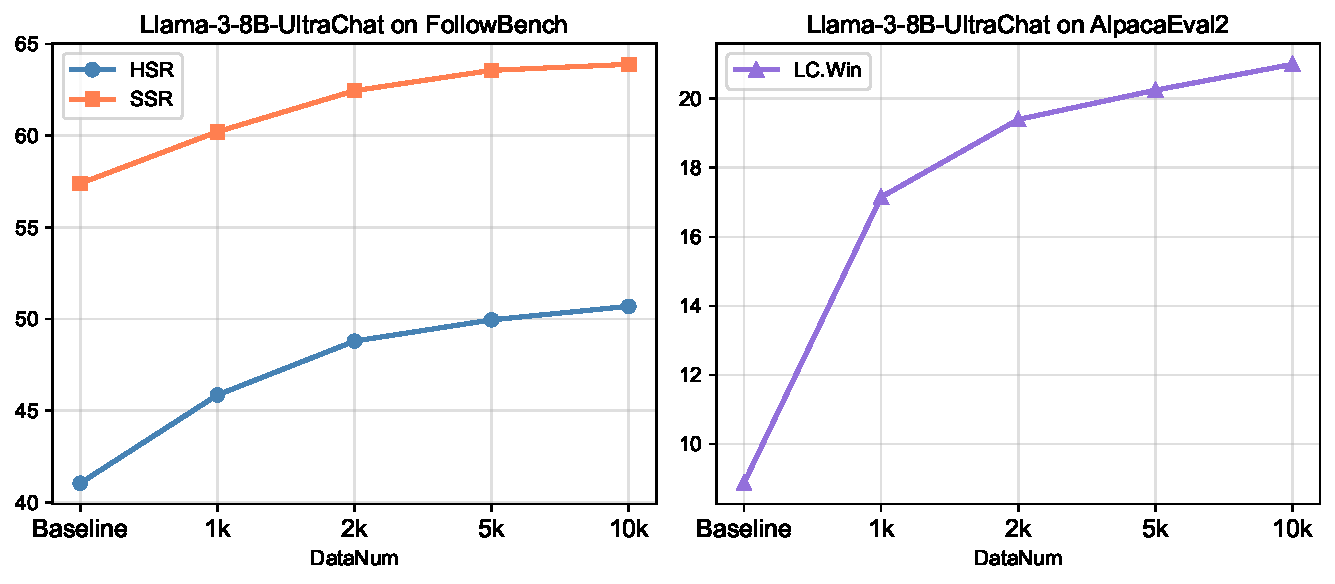
\includegraphics[width=0.95\linewidth]{source/data_visualization/llama_UltraChat_DataNum.pdf}
% }
% \subfigure[Llama-3-8B-Tulu]{
%     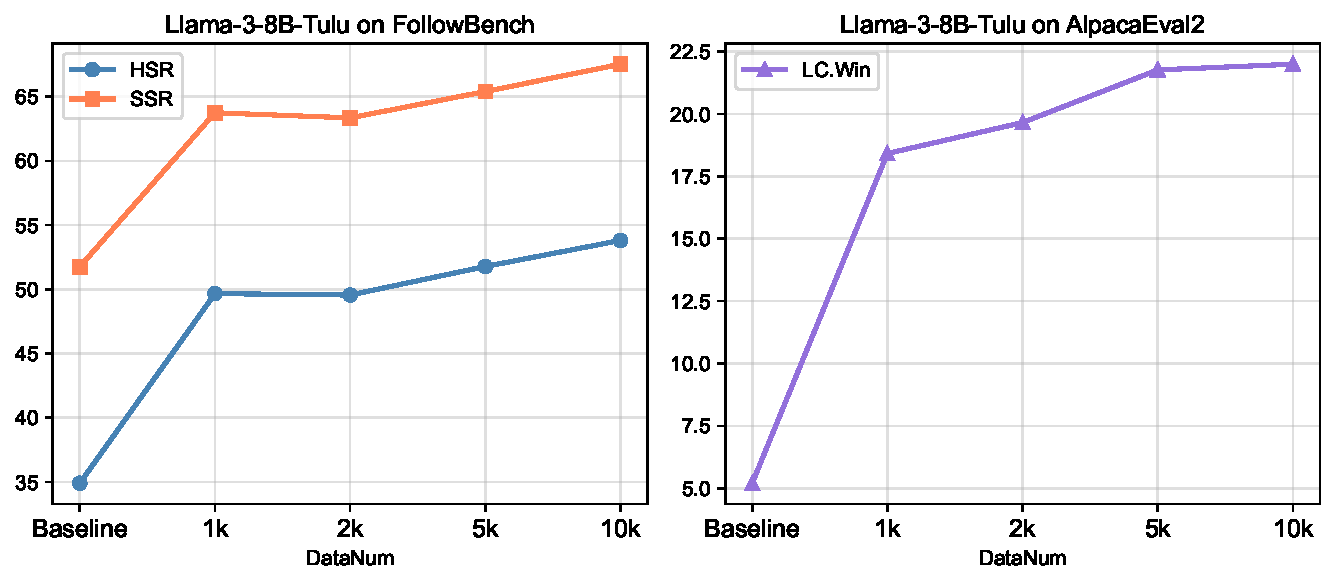
\includegraphics[width=0.95\linewidth]{source/data_visualization/llama_Tulu_DataNum.pdf}
% }
% \vspace{-3mm}
% \caption{The variation of performance on FollowBench and AlpacaEval2 with the variation of data number.}
% \vspace{-3mm}
% \label{figure:data_num}
% \end{figure}

\subsection{Impact on Fundamental Capabilities}

Previous methods have indicated LLMs may suffer from capability degradation during preference alignment phase, which is also known as alignment tax ~\citep{ouyang2022training}. To evaluate this concern, we tested our DIR method on several fundamental capability benchmarks: 1) World Knowledge: MMLU \citep{hendrycks2021measuring}; 2) Commonsense Reasoning: CommonsenseQA (CQA) \citep{talmor-etal-2019-commonsenseqa} and Natural Questions (NQ) \citep{kwiatkowski2019natural}; 3) Coding: HumanEval \citep{chen2021evaluatinglargelanguagemodels}; and 4) Mathematics: GSM8K \citep{cobbe2021trainingverifierssolvemath}. 

\begin{figure*}[pos=tbp]
\centering
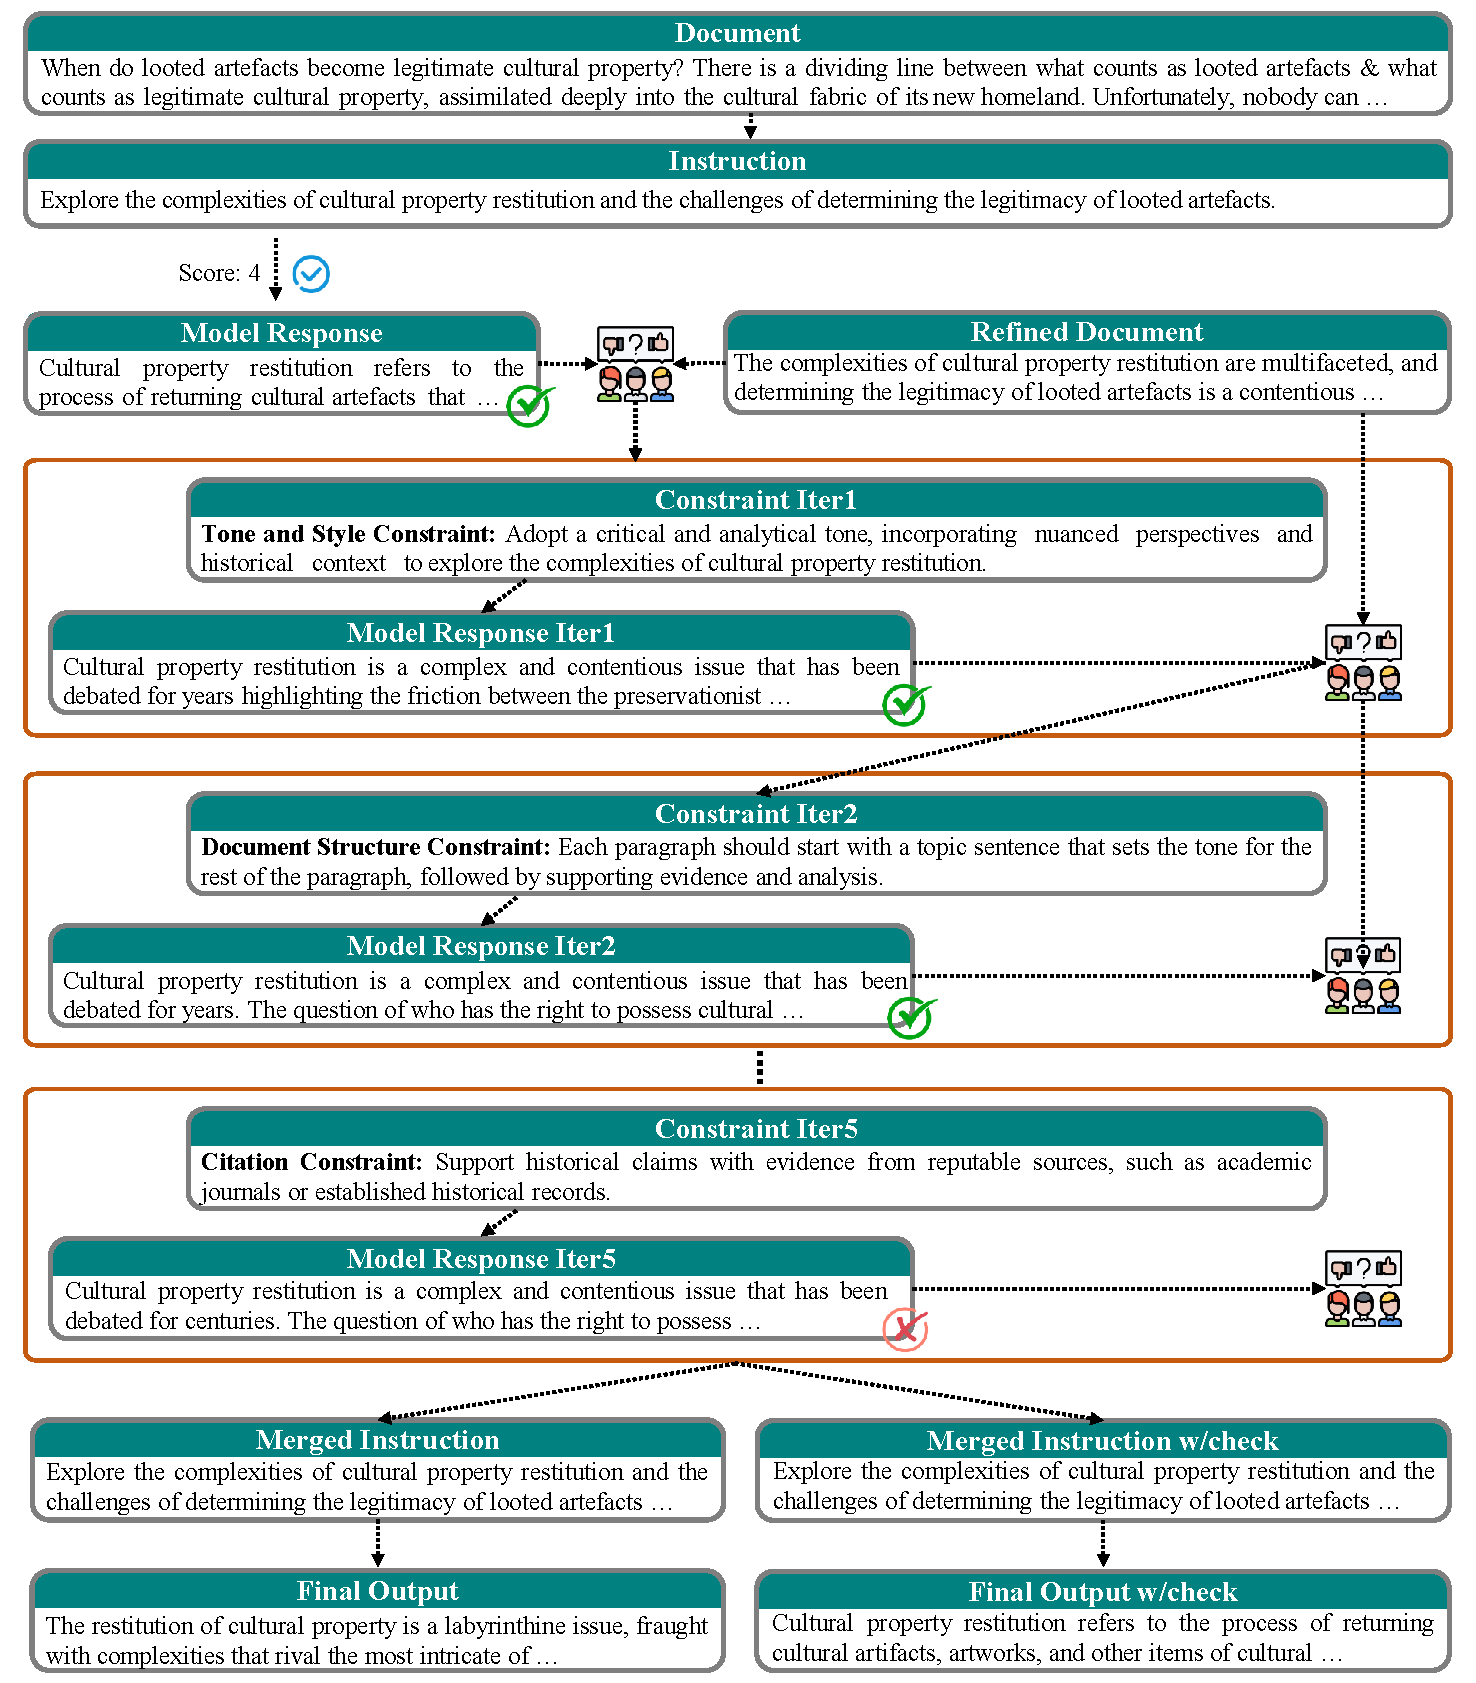
\includegraphics[width=0.88\linewidth]{source/pipeline_demo.pdf}
\caption{An End-to-End Document-grounded Iterative Refinement Example.}
\label{figure:pipeline_case}
\end{figure*}

\begin{table*}[t]
\centering
\caption{Evaluation results of fundamental capabilities of models optimized by DIR.}
\renewcommand{\arraystretch}{0.95}
\resizebox{0.8\textwidth}{!}{
\begin{tabular}{l|l|ccccc|c}
\toprule
\textbf{Base Model} & \textbf{Method} & \textbf{MMLU} & \textbf{CQA} & \textbf{NQ} & \textbf{HumanEval} & \textbf{GSM8K} & \textbf{AVG} \\
\midrule
\multirow{3}{*}{Llama-3-8B-UltraChat} 
& Baseline & 64.00 & 72.97 & 29.61 & 30.49 & 57.47 & 50.90 \\
& DIR-SFT & 61.64 & 73.63 & 30.54 & 29.88 & 54.59 & 50.05 \\
& DIR-RL & 63.48 & 74.15 & 31.27 & 29.53 & 58.29 & \textbf{51.34} \\
\midrule
\multirow{2}{*}{Qwen-2.5-7B-UltraChat} 
& Baseline & 73.64 & 82.39 & 25.68 & 52.20 & 81.65 & 63.11 \\
& DIR-SFT & 73.35 & 82.56 & 25.76 & 55.49 & 84.38 & 64.30 \\
& DIR-RL & 73.51 & 83.42 & 25.23 & 56.68 & 85.51 & \textbf{64.87} \\
\midrule
\multirow{2}{*}{Llama-3-8B-Tulu} 
& Baseline & 65.43 & 79.44 & 32.22 & 50.61 & 64.14 & 58.36 \\
& DIR-SFT & 64.95 & 79.92 & 34.62 & 50.85 & 63.70 & \textbf{58.80} \\
& DIR-RL & 64.27 & 79.13 & 31.56 & 51.18 & 63.41 & 57.91  \\
\bottomrule
\end{tabular}}
\label{table:fundamental}
\end{table*}

As shown in Table \ref{table:fundamental}, our method does not have a negative impact on fundamental capabilities. Specifically, DIR-RL improves the average performance of Llama-3-8B-UltraChat and Qwen-2.5-7B-UltraChat by 0.44 and 1.76 points, respectively. Similarly, DIR-SFT shows improvements on Qwen-2.5-7B-UltraChat and Llama-3-8B-Tulu by 1.19 and 0.44 points. This indicates that instructions synthesized from documents with evenly sampled distributions also exhibit even distribution, which is helpful for maintaining the fundamental knowledge and capabilities acquired during pre-train stage.

% \subsection{Robustness to Document Quality}

% \begin{table}[t]
% \centering
% \caption{Comparison of model performance when fine-tuned on instructions from different document sets.}
% \renewcommand{\arraystretch}{1.0}
% \resizebox{0.48\textwidth}{!}{
% \begin{tabular}{c|ccc|cc|cc}
% \toprule
% \multirow{2}{*}{\textbf{Data}} & \multicolumn{3}{c|}{\textbf{CFBench}} & \multicolumn{2}{c|}{\textbf{FollowBench}} & \multicolumn{2}{c}{\textbf{AlpacaEval2}} \\
% & \textbf{CSR} & \textbf{ISR} & \textbf{PSR} & \textbf{HSR} & \textbf{SSR} & \textbf{LC.} & \textbf{Len} \\
% \midrule
% random 1k & 0.61	& 0.23	& 0.33	& 45.85	& 60.21	& 17.15	& 1,611 \\
% low-quality 1k	& 0.60	& 0.22	& 0.30	& 44.00	& 59.83	& 16.10	& 1,685 \\
% \bottomrule
% \end{tabular}}
% \label{table:Robustness}
% \end{table}

% As discussed in Section \ref{sec:IIR}, our framework primarily utilizes documents to extract constraints rather than as direct fine-tuning targets. During fine-tuning, we use outputs from the guidance model as targets, which insulates the process from document quality issues. Moreover, we implemented multiple safeguards in our data production pipeline, which provides inherent robustness against document noise.

% To empirically validate our method's robustness to document quality, we conducted an additional experiment comparing two document sets: (1) a "low-quality" subset comprising the 1,000 lowest-scoring documents from DIR-10k (evaluated by GPT-4 across helpfulness, completeness, and harmlessness dimensions), and (2) a randomly sampled set of 1,000 documents from the same corpus.

% Table \ref{table:Robustness} presents the performance comparison of Llama-3-8B-UltraChat models fine-tuned on instructions derived from these two document sets. The results demonstrate negligible performance differences across all evaluation benchmarks. This empirical evidence confirms that our method maintains consistent performance regardless of input document quality, validating its robustness.

% Additionally, we provide the number of samples at each stage of the iterative process. As shown in Table \ref{table:Efficiency}, despite starting with a large number of initial documents, only 15\% of them are retained for iterative instruction refinement. Furthermore, nearly 50\% of the documents are filtered out during the iterations, leaving only the highest-quality samples for final training. This demonstrates how our carefully designed strategies effectively maintain sample quality across multiple iterations.

% \begin{table}[t]
% \centering
% \caption{Progressive reduction in sample size through filtering stages and five iterations.}
% \renewcommand{\arraystretch}{0.95}
% \resizebox{0.4\textwidth}{!}{
% \begin{tabular}{c|c}
% \toprule
% \textbf{Stage} & \textbf{Sample Number}\\
% \midrule
% Rule-based Filtering & 300k \\
% Density-based Sampling	& 60k \\
% Instruction Scoring	& 20k \\
% Iteration 1	& 17.3k \\
% Iteration 2	& 15.2k \\
% Iteration 3	& 13.7k \\
% Iteration 4	& 12.7k \\
% Iteration 5	& 11.9k \\
% \bottomrule
% \end{tabular}}
% \label{table:Efficiency}
% \end{table}

% \subsection{Influence of Guidance Model Size}
% \label{sec:Guidance_Model_Size}

% \begin{table}[!t]
% \centering
% \caption{Experiment results on Qwen-2.5-7B-UltraChat fine-tuned with different guidance model size.}
% \renewcommand{\arraystretch}{0.95}
% \resizebox{0.4\textwidth}{!}{
% \begin{tabular}{c|cc|cc}
% \toprule
% \multirow{2}{*}{\textbf{Guid. Model}} & \multicolumn{2}{c}{\textbf{FollowBench}} & \multicolumn{2}{c}{\textbf{AlpacaEval2}} \\
% & \textbf{HSR}   & \textbf{SSR}   & \textbf{LC.}      & \textbf{Len}  \\
% \midrule
% \begin{tabular}[c]{@{}c@{}}Baseline\end{tabular}  & 47.71    & 64.79  & 10.87   & 836   \\
% \midrule
% 14B     & 57.72   & 70.59   & 29.13   & 1,501   \\
% 32B     & \textbf{60.06}   & \textbf{71.97}   & 26.39   & 1,309    \\
% 72B     & 59.07   & 71.35   & \textbf{32.43}  & 1,779     \\
% \bottomrule
% \end{tabular}}
% \label{table:guidance_size}
% \end{table}

% In Table \ref{table:guidance_size}, we investigate the impact of guidance model size on DIR's performance. We performed experiments with Qwen-2.5-7B-UltraChat as the base model, while varying the guidance model size from 14B to 72B parameters. As shown, all guidance models with different sizes significantly improve instruction-following ability compared to the baseline, while larger models generally provide greater improvement. On the other hand, even the 14B guidance model demonstrates remarkable improvement. This scalability across different model sizes highlights the robustness and efficiency of our proposed approach.

% which leverages documents as reference to help the constraint generation process.

% These findings suggest that DIR's effectiveness is not strictly dependent on large guidance models. The method effectively leverages both document knowledge and model knowledge through judging mechanism to generate meaningful constraints, making it practical and efficient even with relatively smaller guidance models. 

\subsection{Case Study}

% This section presents a detailed end-to-end demonstration of our pipeline in Figure \ref{figure:pipeline_case}. The case study provides a thorough walkthrough of each stage in our instruction generation and refinement process.

To intuitively demonstrate how the DIR framework transforms unstructured documents into high-quality complex instructions, we provide an end-to-end example in Figure \ref{figure:pipeline_case}. As shown, through the document-grounded iterative refinement process, a complex instruction incorporating multifaceted constraints, including tone, structure, and citation requirements, is ultimately synthesized. This demonstrates that the DIR framework can effectively mine implicit human preferences within documents and transform them into explicit complex alignment signals.
\section{Conclusion}
This paper presents Document-grounded Iterative Refinement (DIR), a novel framework for synthesizing complex instructions that closely mirror real-world scenarios. Building on this, we propose a dual-stage constraint-aware optimization pipeline, integrating constraint-aware SFT with RL. Empirical results demonstrate that DIR significantly enhances instruction alignment across a diverse range of models.

While previous methods for complex instruction following often introduce constraints without clear justification, it is crucial to understand what authentic complex instruction entails. In the future, we will conduct further research on the effectiveness and efficiency of complex instruction data.

\section*{CRediT authorship contribution statement}
\textbf{Wei Liu:} Methodology, Software, Validation, Formal analysis, Writing -- review \& editing.

\textbf{Hui Huang:} Conceptualization, Methodology, Software, Validation, Formal analysis, Investigation, Data curation, Visualization, Writing -- original draft, Writing -- review \& editing.

\textbf{Kehai Chen:} Methodology, Investigation, Writing -- review \& editing.

\textbf{Jiaheng Liu:} Methodology, Writing -- review \& editing.

\textbf{Yancheng He:} Software, Investigation, Data curation.

\textbf{Lvyuan Han:} Investigation, Data curation.

\textbf{Wenhao Jiang:} Validation, Writing -- review \& editing.

\textbf{Muyun Yang:} Supervision, Validation, Writing -- review \& editing.

\textbf{Zhaoxiang Zhang:} Supervision, Writing -- review \& editing.

\textbf{Tiejun Zhao:} Supervision, Project administration.

\section*{Declaration of Competing Interest}
The authors declare that they have no known competing financial interests or personal relationships that could have appeared to influence the work reported in this paper.

\section*{Acknowledgements}
This work was supported by the National Key R\&D Program of China (Grant No. 2024YFC3809100), the National Natural Science Foundation of China (Grant No. 62276077, 62376075, 62376076), the Natural Science Foundation of Heilongjiang Province (Grant No. ZL2025F004), and the MOE Key Laboratory of Cognitive Intelligence and Content Security (Grant No. 10120251103, Harbin Institute of Technology).

\clearpage

% The appendix is retained for a later decision on supplementary material.
% \appendix
% \clearpage
\onecolumn

\section{Additional Experiments}
\label{appendix:additional_experiments}

\subsection{Case Study for Complete Pipeline}
\label{appendix:pipeline_case}

\begin{figure}[ht]
\centering
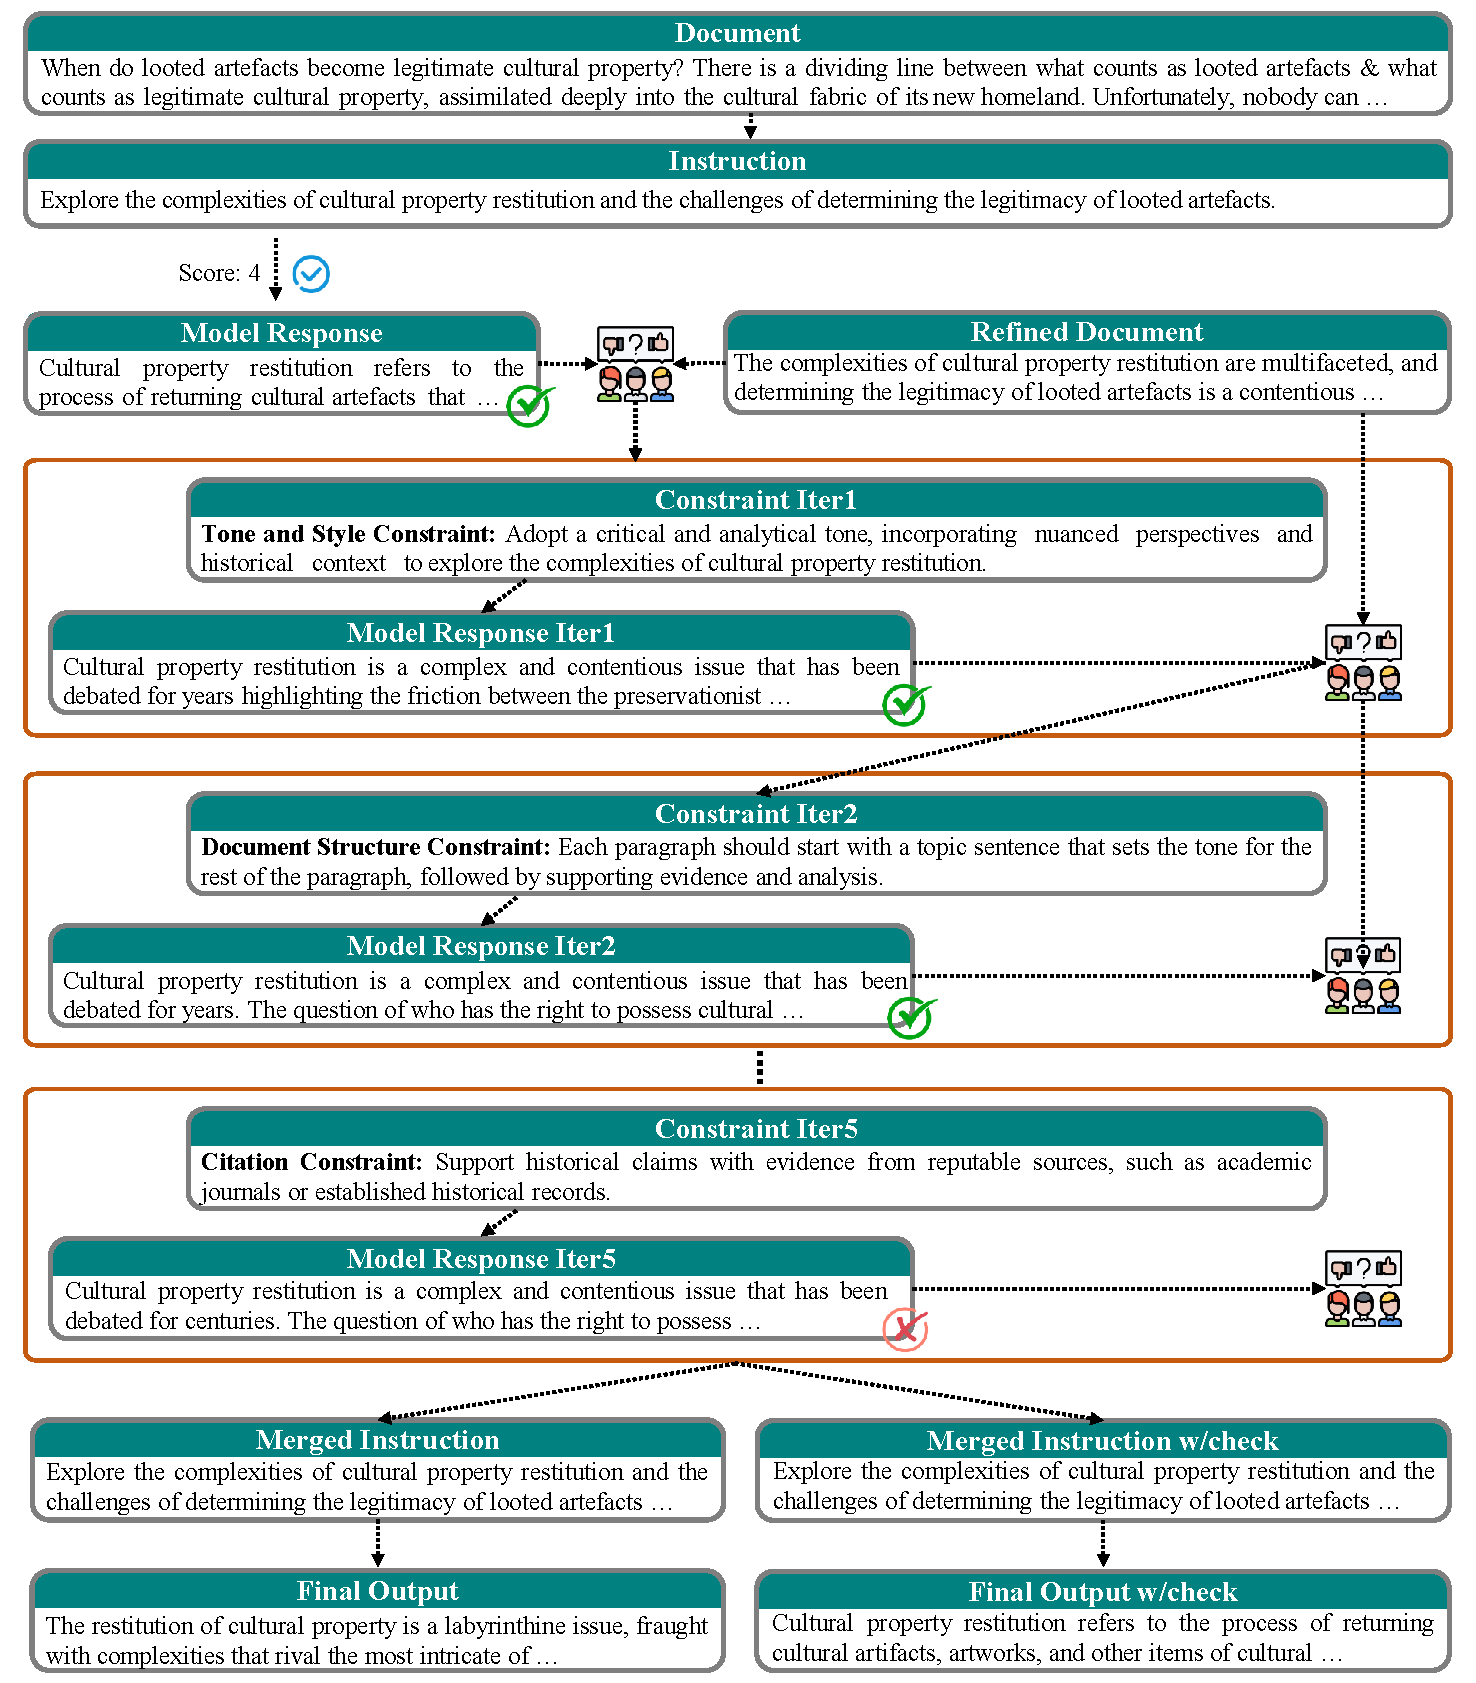
\includegraphics[width=0.75\linewidth]{source/pipeline_demo.pdf}
\caption{End-to-End Pipeline Implementation Example.}
\label{figure:appendix_pipeline_case}
\end{figure}

This section presents a detailed end-to-end demonstration of our pipeline in Figure \ref{figure:appendix_pipeline_case}. The case study provides a thorough walkthrough of each stage in our instruction generation and refinement process.

\subsection{Controlled Comparison of Instruction Synthesis Method}
\label{appendix:controlled_comparison}

Despite the superior performance reflected in Table \ref{table:main_results}, the fine-tuned results can be influenced by confounding variables. To isolate the direct impact of the instruction data quality, we conducted an additional set of experiments under a strictly controlled environment. In this setting, we re-generated datasets for all baseline methods using the identical source corpus (\textbf{Dolma v1.7}) and guidance model (\textbf{Llama-3-70B-Instruct}) employed in our DIR framework. After that, we performed SFT on the same base model with the same hyper-parameters. This ensures a direct "apples-to-apples" comparison of different instruction synthesis methods.

\begin{table}[!ht]
\centering
\caption{SFT Performance comparison under controlled experimental settings on Llama-3-8B-UltraChat. All methods are implemented with the same source document corpus (Dolma v1.7) and guidance model (Llama-3-70B-Instruct).}
\renewcommand{\arraystretch}{1.05}
\resizebox{0.9\textwidth}{!}{
\begin{tabular}{lc|ccc|cc|cc}
\toprule
\multirow{2}{*}{\textbf{Method}} & \multirow{2}{*}{\textbf{Setting}} & \multicolumn{3}{c|}{\textbf{CFBench}} & \multicolumn{2}{c|}{\textbf{FollowBench}} & \multicolumn{2}{c}{\textbf{AlpacaEval2}} \\
& & \textbf{CSR} & \textbf{ISR} & \textbf{PSR} & \textbf{HSR} & \textbf{SSR} & \textbf{LC.} & \textbf{Len} \\
\midrule
Baseline & - & 0.51 & 0.15 & 0.22 & 41.04 & 57.39 & 8.86 & 1,017 \\
Back-translation-10K & Original & $\text{0.40}_{\textcolor{deepred}{\text{-0.11}}}$ & $\text{0.11}_{\textcolor{deepred}{\text{-0.04}}}$ & $\text{0.15}_{\textcolor{deepred}{\text{-0.07}}}$ & $\text{21.19}_{\textcolor{deepred}{\text{-19.85}}}$ & $\text{33.92}_{\textcolor{deepred}{\text{-23.47}}}$ & $\text{0.96}_{\textcolor{deepred}{\text{-7.90}}}$ & 2,966 \\
Back-and-forth-10K & Original & $\text{0.58}_{\textcolor{deepgreen}{\text{+0.07}}}$ & $\text{0.20}_{\textcolor{deepgreen}{\text{+0.05}}}$ & $\text{0.27}_{\textcolor{deepgreen}{\text{+0.05}}}$ & $\text{44.65}_{\textcolor{deepgreen}{\text{+3.61}}}$ & $\text{61.58}_{\textcolor{deepgreen}{\text{+4.19}}}$ & $\text{10.06}_{\textcolor{deepgreen}{\text{+1.20}}}$ & 1,440 \\
ShareGPT-10K & Re-run & $\text{0.59}_{\textcolor{deepgreen}{\text{+0.08}}}$ & $\text{0.20}_{\textcolor{deepgreen}{\text{+0.05}}}$ & $\text{0.31}_{\textcolor{deepgreen}{\text{+0.09}}}$ & $\text{44.50}_{\textcolor{deepgreen}{\text{+3.46}}}$ & $\text{59.20}_{\textcolor{deepgreen}{\text{+1.81}}}$ & $\text{12.70}_{\textcolor{deepgreen}{\text{+3.84}}}$ & 1,570 \\
Self-Instruct-10K & Re-run & $\text{0.42}_{\textcolor{deepred}{\text{-0.09}}}$ & $\text{0.11}_{\textcolor{deepred}{\text{-0.04}}}$ & $\text{0.16}_{\textcolor{deepred}{\text{-0.06}}}$ & $\text{15.00}_{\textcolor{deepred}{\text{-26.04}}}$ & $\text{32.00}_{\textcolor{deepred}{\text{-25.39}}}$ & $\text{8.50}_{\textcolor{deepred}{\text{-0.36}}}$ & 2,384 \\
Evol-Instruct-10K & Re-run & $\text{0.55}_{\textcolor{deepgreen}{\text{+0.04}}}$ & $\text{0.21}_{\textcolor{deepgreen}{\text{+0.06}}}$ & $\text{0.26}_{\textcolor{deepgreen}{\text{+0.04}}}$ & $\text{45.20}_{\textcolor{deepgreen}{\text{+4.16}}}$ & $\text{59.80}_{\textcolor{deepgreen}{\text{+2.41}}}$ & $\text{8.80}_{\textcolor{deepred}{\text{-0.06}}}$ & 890 \\
MUFFIN-10K & Re-run & $\text{0.48}_{\textcolor{deepred}{\text{-0.03}}}$ & $\text{0.15}_{\textcolor{deepgreen}{\text{+0.00}}}$ & $\text{0.20}_{\textcolor{deepred}{\text{-0.02}}}$ & $\text{29.50}_{\textcolor{deepred}{\text{-11.54}}}$ & $\text{46.20}_{\textcolor{deepred}{\text{-11.19}}}$ & $\text{4.01}_{\textcolor{deepred}{\text{-4.85}}}$ & 990 \\
Conifer-10K & Re-run & $\text{0.52}_{\textcolor{deepgreen}{\text{+0.01}}}$ & $\text{0.18}_{\textcolor{deepgreen}{\text{+0.03}}}$ & $\text{0.23}_{\textcolor{deepgreen}{\text{+0.01}}}$ & $\text{43.20}_{\textcolor{deepgreen}{\text{+2.16}}}$ & $\text{58.50}_{\textcolor{deepgreen}{\text{+1.11}}}$ & $\text{11.50}_{\textcolor{deepgreen}{\text{+2.64}}}$ & 850 \\
I-SHEEP-10K & Re-run & $\text{0.55}_{\textcolor{deepgreen}{\text{+0.04}}}$ & $\text{0.18}_{\textcolor{deepgreen}{\text{+0.03}}}$ & $\text{0.25}_{\textcolor{deepgreen}{\text{+0.03}}}$ & $\text{36.00}_{\textcolor{deepred}{\text{-5.04}}}$ & $\text{52.50}_{\textcolor{deepred}{\text{-4.89}}}$ & $\text{7.20}_{\textcolor{deepred}{\text{-1.66}}}$ & 1,070 \\
Suri-10K & Re-run & $\text{0.53}_{\textcolor{deepgreen}{\text{+0.02}}}$ & $\text{0.17}_{\textcolor{deepgreen}{\text{+0.02}}}$ & $\text{0.23}_{\textcolor{deepgreen}{\text{+0.01}}}$ & $\text{43.00}_{\textcolor{deepgreen}{\text{+1.96}}}$ & $\text{58.08}_{\textcolor{deepgreen}{\text{+0.69}}}$ & $\text{9.50}_{\textcolor{deepgreen}{\text{+0.64}}}$ & 1,980 \\
Crab-10K & Re-run & $\text{0.54}_{\textcolor{deepgreen}{\text{+0.03}}}$ & $\text{0.17}_{\textcolor{deepgreen}{\text{+0.02}}}$ & $\text{0.23}_{\textcolor{deepgreen}{\text{+0.01}}}$ & $\text{38.50}_{\textcolor{deepred}{\text{-2.54}}}$ & $\text{55.50}_{\textcolor{deepred}{\text{-1.89}}}$ & $\text{8.80}_{\textcolor{deepred}{\text{-0.06}}}$ & 1,105 \\
\textbf{DIR-10K} & Re-run & \textbf{$\text{0.61}_{\textcolor{deepgreen}{\text{+0.10}}}$} & \textbf{$\text{0.24}_{\textcolor{deepgreen}{\text{+0.09}}}$} & \textbf{$\text{0.31}_{\textcolor{deepgreen}{\text{+0.09}}}$} & \textbf{$\text{50.69}_{\textcolor{deepgreen}{\text{+9.65}}}$} & \textbf{$\text{63.89}_{\textcolor{deepgreen}{\text{+6.50}}}$} & \textbf{$\text{21.00}_{\textcolor{deepgreen}{\text{+12.14}}}$} & 1,813 \\
\bottomrule
\end{tabular}}
\label{table:controlled_comparison}
\end{table}

As shown in Table \ref{table:controlled_comparison}, DIR-10K consistently outperforms other synthesis methods across both complex and general instruction benchmarks under controlled conditions. This confirms that the observed gains on instruction following are attributable to the data synthesis method rather than the initial choice of data or models. Notably, the results also reveal the sensitivity of different methods to initial configurations: while Self-Instruct and Suri scaled effectively with our source corpus, other methods such as Conifer and Crab showed diminished performance, suggesting their original performance may have benefited from specific private data distributions.

Meanwhile, robust methods like Evol-Instruct and ShareGPT performed comparably, suggesting their original configurations were already strong.

In summary, this controlled analysis provides stronger evidence for the effectiveness of the DIR framework, demonstrating that its advantages are attributable to the methodology itself rather than the initial choice of data or models.

\subsection{Impact on Fundamental Capabilities}

Previous methods have indicated LLMs may suffer from capability degradation during preference alignment phase, which is also known as alignment tax ~\cite{ouyang2022training}. To evaluate this concern, we tested our DIR method on several fundamental capability benchmarks: 1) World Knowledge: MMLU \cite{hendrycks2021measuring}; 2) Commonsense Reasoning: CommonsenseQA (CQA) \cite{talmor-etal-2019-commonsenseqa} and Natural Questions (NQ) \cite{kwiatkowski2019natural}; 3) Coding: HumanEval \cite{chen2021evaluatinglargelanguagemodels}; and 4) Mathematics: GSM8K \cite{cobbe2021trainingverifierssolvemath}.

\begin{table}[!ht]
\centering
\caption{Evaluation results of fundamental capabilities of models optimized by DIR.}
\renewcommand{\arraystretch}{0.95}
\resizebox{0.8\textwidth}{!}{
\begin{tabular}{l|l|ccccc|c}
\toprule
\textbf{Base Model} & \textbf{Method} & \textbf{MMLU} & \textbf{CQA} & \textbf{NQ} & \textbf{HumanEval} & \textbf{GSM8K} & \textbf{AVG} \\
\midrule
\multirow{3}{*}{Llama-3-8B-UltraChat}
& Baseline & 64.00 & 72.97 & 29.61 & 30.49 & 57.47 & 50.90 \\
& DIR-SFT & 61.64 & 73.63 & 30.54 & 29.88 & 54.59 & 50.05 \\
& DIR-RL & 63.48 & 74.15 & 31.27 & 29.53 & 58.29 & \textbf{51.34} \\
\midrule
\multirow{2}{*}{Qwen-2.5-7B-UltraChat}
& Baseline & 73.64 & 82.39 & 25.68 & 52.20 & 81.65 & 63.11 \\
& DIR-SFT & 73.35 & 82.56 & 25.76 & 55.49 & 84.38 & 64.30 \\
& DIR-RL & 73.51 & 83.42 & 25.23 & 56.68 & 85.51 & \textbf{64.87} \\
\midrule
\multirow{2}{*}{Llama-3-8B-Tulu}
& Baseline & 65.43 & 79.44 & 32.22 & 50.61 & 64.14 & 58.36 \\
& DIR-SFT & 64.95 & 79.92 & 34.62 & 50.85 & 63.70 & \textbf{58.80} \\
& DIR-RL & 64.27 & 79.13 & 31.56 & 51.18 & 63.41 & 57.91  \\
\bottomrule
\end{tabular}}
\label{table:fundamental}
\end{table}

As shown in Table \ref{table:fundamental}, our method does not have a negative impact on fundamental capabilities. Specifically, DIR-RL improves the average performance of Llama-3-8B-UltraChat and Qwen-2.5-7B-UltraChat by 0.44 and 1.76 points, respectively. Similarly, DIR-SFT shows improvements on Qwen-2.5-7B-UltraChat and Llama-3-8B-Tulu by 1.19 and 0.44 points. This indicates that instructions synthesized from documents with evenly sampled distributions also exhibit even distribution, which is helpful for maintaining the fundamental knowledge and capabilities acquired during pre-train stage.

% \subsection{Robustness to Document Quality}

% \begin{table}[!ht]
% \centering
% \caption{Comparison of model performance when fine-tuned on instructions from different document sets.}
% \renewcommand{\arraystretch}{1.0}
% \resizebox{0.48\textwidth}{!}{
% \begin{tabular}{c|ccc|cc|cc}
% \toprule
% \multirow{2}{*}{\textbf{Data}} & \multicolumn{3}{c|}{\textbf{CFBench}} & \multicolumn{2}{c|}{\textbf{FollowBench}} & \multicolumn{2}{c}{\textbf{AlpacaEval2}} \\
% & \textbf{CSR} & \textbf{ISR} & \textbf{PSR} & \textbf{HSR} & \textbf{SSR} & \textbf{LC.} & \textbf{Len} \\
% \midrule
% random 1k & 0.61	& 0.23	& 0.33	& 45.85	& 60.21	& 17.15	& 1,611 \\
% low-quality 1k	& 0.60	& 0.22	& 0.30	& 44.00	& 59.83	& 16.10	& 1,685 \\
% \bottomrule
% \end{tabular}}
% \label{table:Robustness}
% \end{table}

% As discussed in Section \ref{sec:IIR}, our framework primarily utilizes documents to extract constraints rather than as direct fine-tuning targets. During fine-tuning, we use outputs from the guidance model as targets, which insulates the process from document quality issues. Moreover, we implemented multiple safeguards in our data production pipeline, which provides inherent robustness against document noise.

% To empirically validate our method's robustness to document quality, we conducted an additional experiment comparing two document sets: (1) a "low-quality" subset comprising the 1,000 lowest-scoring documents from DIR-10k (evaluated by GPT-4 across helpfulness, completeness, and harmlessness dimensions), and (2) a randomly sampled set of 1,000 documents from the same corpus.

% Table \ref{table:Robustness} presents the performance comparison of Llama-3-8B-UltraChat models fine-tuned on instructions derived from these two document sets. The results demonstrate negligible performance differences across all evaluation benchmarks. This empirical evidence confirms that our method maintains consistent performance regardless of input document quality, validating its robustness.

% Additionally, we provide the number of samples at each stage of the iterative process. As shown in Table \ref{table:Efficiency}, despite starting with a large number of initial documents, only 15\% of them are retained for iterative instruction refinement. Furthermore, nearly 50\% of the documents are filtered out during the iterations, leaving only the highest-quality samples for final training. This demonstrates how our carefully designed strategies effectively maintain sample quality across multiple iterations.

% \begin{table}[!ht]
% \centering
% \caption{Progressive reduction in sample size through filtering stages and five iterations.}
% \renewcommand{\arraystretch}{0.95}
% \resizebox{0.4\textwidth}{!}{
% \begin{tabular}{c|c}
% \toprule
% \textbf{Stage} & \textbf{Sample Number}\\
% \midrule
% Rule-based Filtering & 300k \\
% Density-based Sampling	& 60k \\
% Instruction Scoring	& 20k \\
% Iteration 1	& 17.3k \\
% Iteration 2	& 15.2k \\
% Iteration 3	& 13.7k \\
% Iteration 4	& 12.7k \\
% Iteration 5	& 11.9k \\
% \bottomrule
% \end{tabular}}
% \label{table:Efficiency}
% \end{table}

\subsection{Influence of Guidance Model Size}
\label{sec:Guidance_Model_Size}

\begin{table}[!ht]
\centering
\caption{Experiment results on Qwen-2.5-7B-UltraChat fine-tuned with different guidance model size.}
\renewcommand{\arraystretch}{0.95}
\resizebox{0.4\textwidth}{!}{
\begin{tabular}{c|cc|cc}
\toprule
\multirow{2}{*}{\textbf{Guid. Model}} & \multicolumn{2}{c}{\textbf{FollowBench}} & \multicolumn{2}{c}{\textbf{AlpacaEval2}} \\
& \textbf{HSR}   & \textbf{SSR}   & \textbf{LC.}      & \textbf{Len}  \\
\midrule
\begin{tabular}[c]{@{}c@{}}Baseline\end{tabular}  & 47.71    & 64.79  & 10.87   & 836   \\
\midrule
14B     & 57.72   & 70.59   & 29.13   & 1,501   \\
32B     & \textbf{60.06}   & \textbf{71.97}   & 26.39   & 1,309    \\
72B     & 59.07   & 71.35   & \textbf{32.43}  & 1,779     \\
\bottomrule
\end{tabular}}
\label{table:guidance_size}
\end{table}

In Table \ref{table:guidance_size}, we investigate the impact of guidance model size on DIR's performance. We performed experiments with Qwen-2.5-7B-UltraChat as the base model, while varying the guidance model size from 14B to 72B parameters. As shown, all guidance models with different sizes significantly improve instruction-following ability compared to the baseline, while larger models generally provide greater improvement. On the other hand, even the 14B guidance model demonstrates remarkable improvement. This scalability across different model sizes highlights the robustness and efficiency of our proposed approach.

These findings suggest that DIR's effectiveness is not strictly dependent on large guidance models. The method effectively leverages both document knowledge and model knowledge through judging mechanism to generate meaningful constraints, making it practical and efficient even with relatively smaller guidance models.

\section{Implementation Details}
\label{appendix:additional_details}

\subsection{Model Training Hyper-parameters}
\label{appendix:hyper-parameters}

This section details our model training configuration. We employed Supervised Fine-Tuning (SFT) based on the LlamaFactory \cite{zheng2024llamafactory} framework, with hyper-parameters as outlined in Table \ref{table:hyperparams}. Furthermore, we conducted Reinforcement Learning (RL) experiments using the verl \cite{verl} framework, and the corresponding hyper-parameters are listed in Table \ref{tab:hyperparams_rl}.

\begin{table}[!ht]
\centering
\renewcommand{\arraystretch}{1.1}
\caption{Hyper-parameters for SFT experiments.}
\resizebox{0.45\textwidth}{!}{
\begin{tabular}{l|cc}
\toprule
\textbf{Configuration} & \textbf{Llama-3-8B}   & \textbf{Qwen-2.5-7B}   \\
\midrule
Max Sequence Length    & 4096                  & 4096                   \\
Learning Rate          & 1e-5                  & 1e-5                   \\
LR Scheduler           & cosine decay          & cosine decay           \\
Training Epochs        & 3                     & 3                      \\
Batch Size             & 64                    & 64                     \\
Mixed Precision        & bf16                  & bf16                   \\
DeepSpeed ZeRO Stage   & stage 2               & stage 2                \\
\bottomrule
\end{tabular}}
\label{table:hyperparams}
\end{table}

\begin{table*}[!ht]
\centering
\renewcommand{\arraystretch}{1.1}
\caption{Hyper-parameters for RL experiments.}
\resizebox{0.50\linewidth}{!}{
\begin{tabular}{lccc}
\toprule
\textbf{Configuration} & \textbf{GRPO} & \textbf{PPO} & \textbf{Reinforce++} \\
\midrule
Generation Batch Size           & 512      & 256      & 256 \\
Training Batch Size             & 256      & 256      & 256 \\
Max Prompt Length               & 1024     & 1024     & 1024 \\
Max Response Length             & 4096     & 4096     & 4096 \\
Actor Learning Rate             & 3e-6     & 3e-6     & 3e-6 \\
Actor Mini Batch Size           & 64       & 64       & 64 \\
Actor Micro Batch Size          & 8        & 8        & 8 \\
Use KL Loss                     & False    & True     & True \\
KL Loss Coefficient             & 0.0      & 0.001    & 0.001 \\
Rollout Log Prob Batch Size     & 16       & 16       & 16 \\
Rollout Number ($N$)            & 8        & --       & 8 \\
Ref Log Prob Batch Size         & 16       & 16       & 16 \\
Critic Learning Rate            & --       & 1e-5     & -- \\
Critic Micro Batch Size         & --       & 8        & -- \\
GPUs Per Node                   & 8        & 8        & 8 \\
Number of Nodes                 & 2        & 2        & 2 \\
Total Epochs                    & 10       & 10       & 10 \\
\bottomrule
\end{tabular}
}
\label{tab:hyperparams_rl}
\end{table*}

\subsection{Prompt Templates}
\label{appendix:prompt_templates}

This section presents the prompts used in our data generation pipeline. For Initial Instruction Generation, the prompts serve different purposes from initial instruction generation through back-translation (Figure~\ref{figure:prompt_back_ins}) to document refining (Figure~\ref{figure:prompt_document_polish}) and instruction scoring (Figure~\ref{figure:prompt_ins_score}). For Iterative Instruction Refinement, the prompts serve different purposes from constraint generation (Figure~\ref{figure:cons_generate}), constraint verification (Figure~\ref{figure:cons_check}), and finally combines all elements into refined instructions (Figure~\ref{figure:cons_combine}).

\subsection{Instruction Score Criteria}
\label{appendix:ins_score_case}

This section presents the detailed score criteria of the instruction quality through representative examples. As illustrated in Figure~\ref{figure:ins_score_case_show}, we provide a diverse set of instructions spanning the entire quality spectrum (scores 1-5). Each score category is exemplified by five carefully selected cases, where score 1 represents basic quality and score 5 demonstrates exceptional quality.

\begin{figure}[ht]
\centering
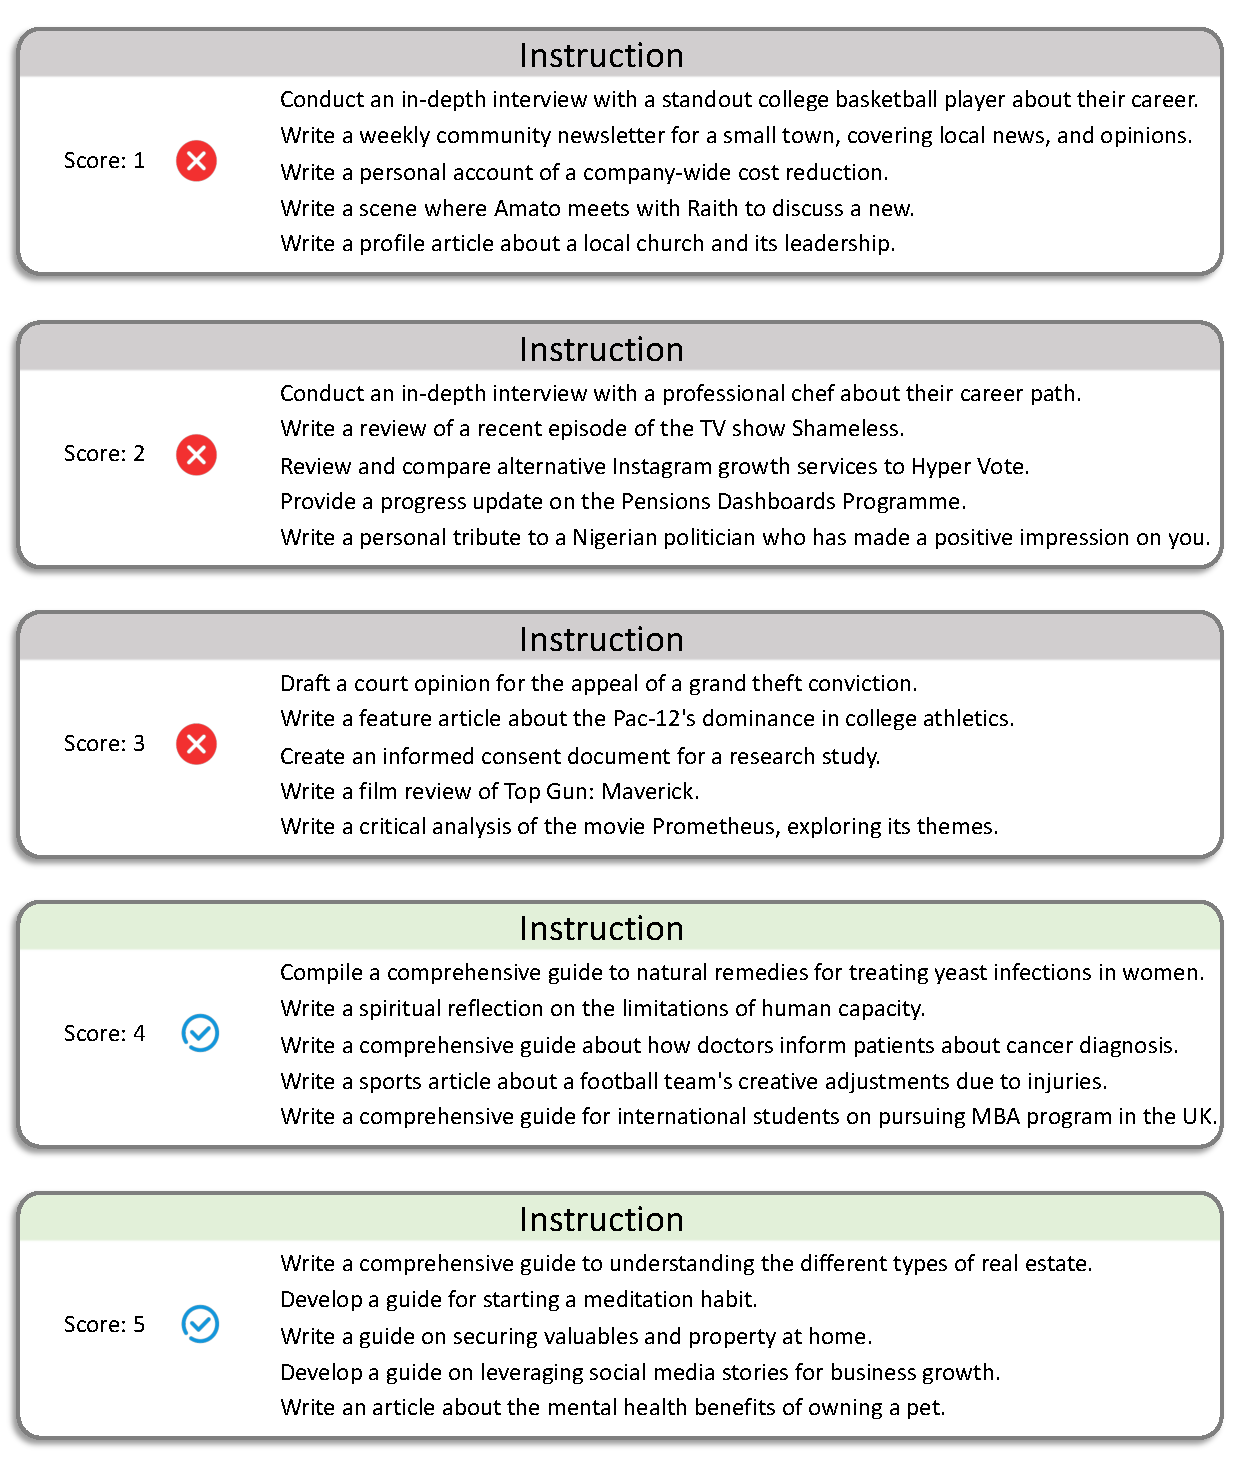
\includegraphics[width=0.75\linewidth]{source/prompt/ins_score_case.pdf}
\caption{Examples of instructions at different score levels (1-5), where each score level is illustrated with five representative cases. Score 1 represents the lowest quality while score 5 represents the highest quality.}
\label{figure:ins_score_case_show}
\end{figure}


\begin{figure}[ht]
\centering
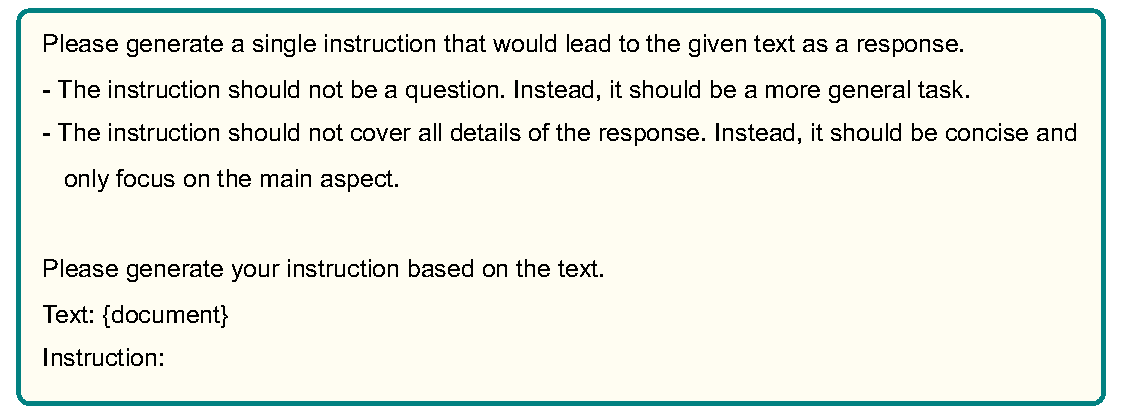
\includegraphics[width=0.8\linewidth]{source/prompt/prompt_back_ins.pdf}
\caption{Prompt for generating initial instructions through back-translation.}
\label{figure:prompt_back_ins}
\end{figure}

\begin{figure}[ht]
\centering
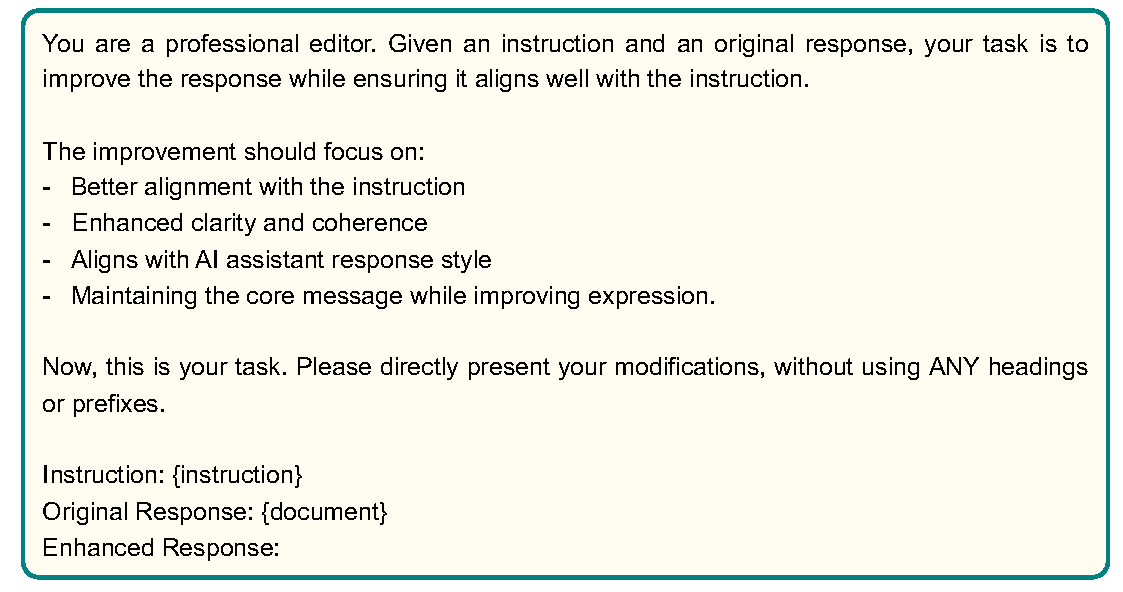
\includegraphics[width=0.8\linewidth]{source/prompt/prompt_document_polish.pdf}
\caption{Prompt for refining document content.}
\label{figure:prompt_document_polish}
\end{figure}

\begin{figure}[ht]
\centering
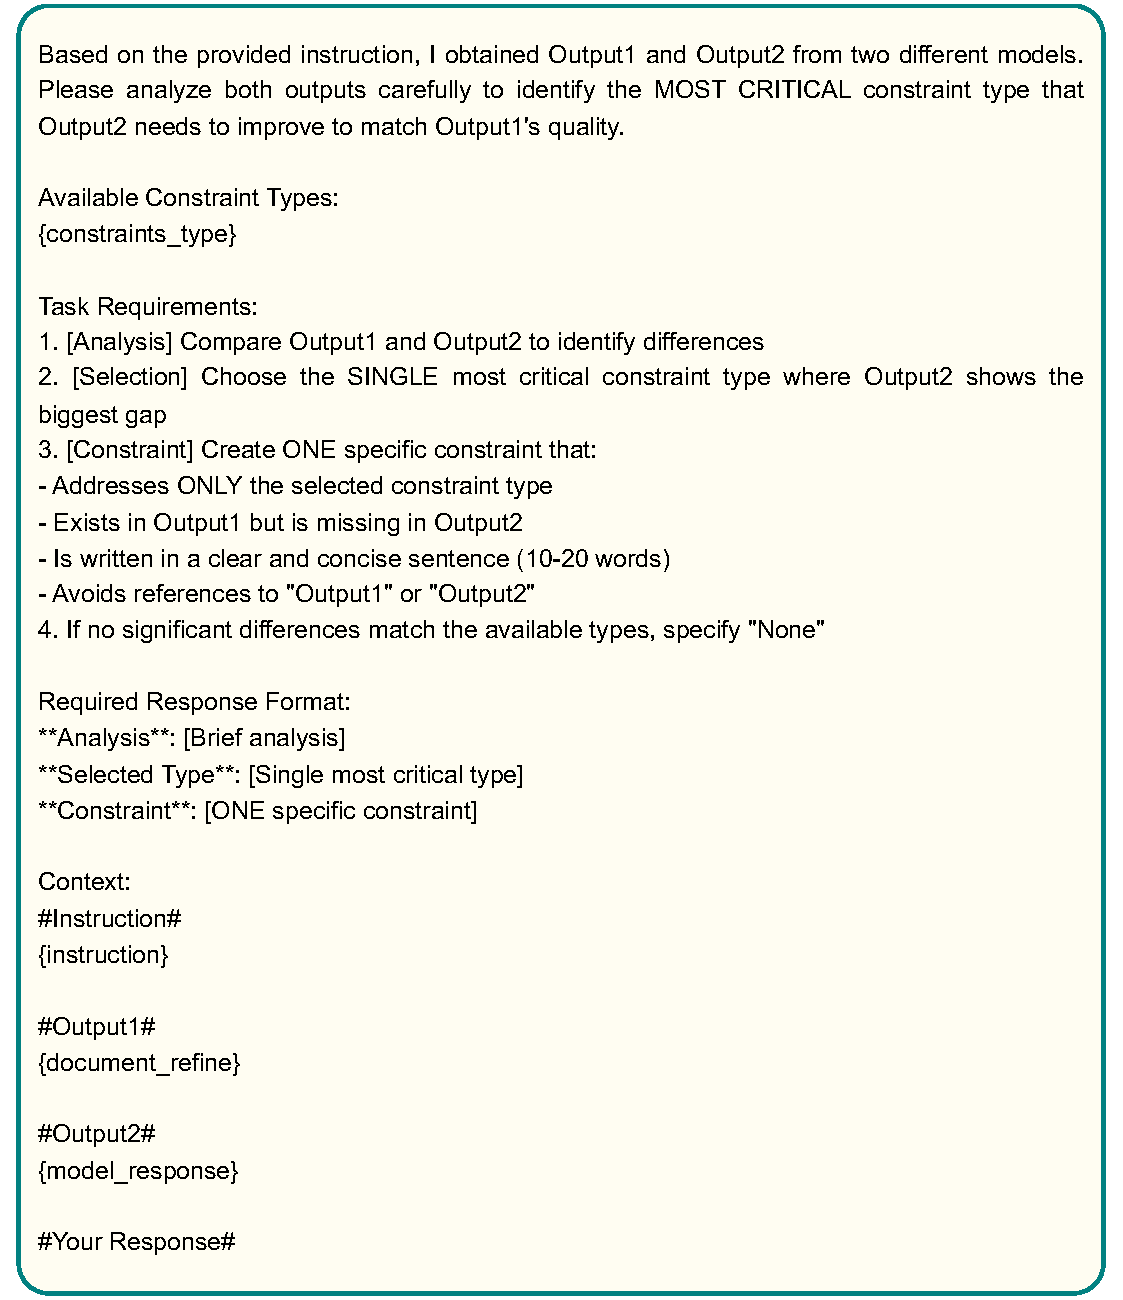
\includegraphics[width=0.8\linewidth]{source/prompt/cons_generate.pdf}
\caption{Prompt for generating constraints based on judge.}
\label{figure:cons_generate}
\end{figure}

\begin{figure}[ht]
\centering
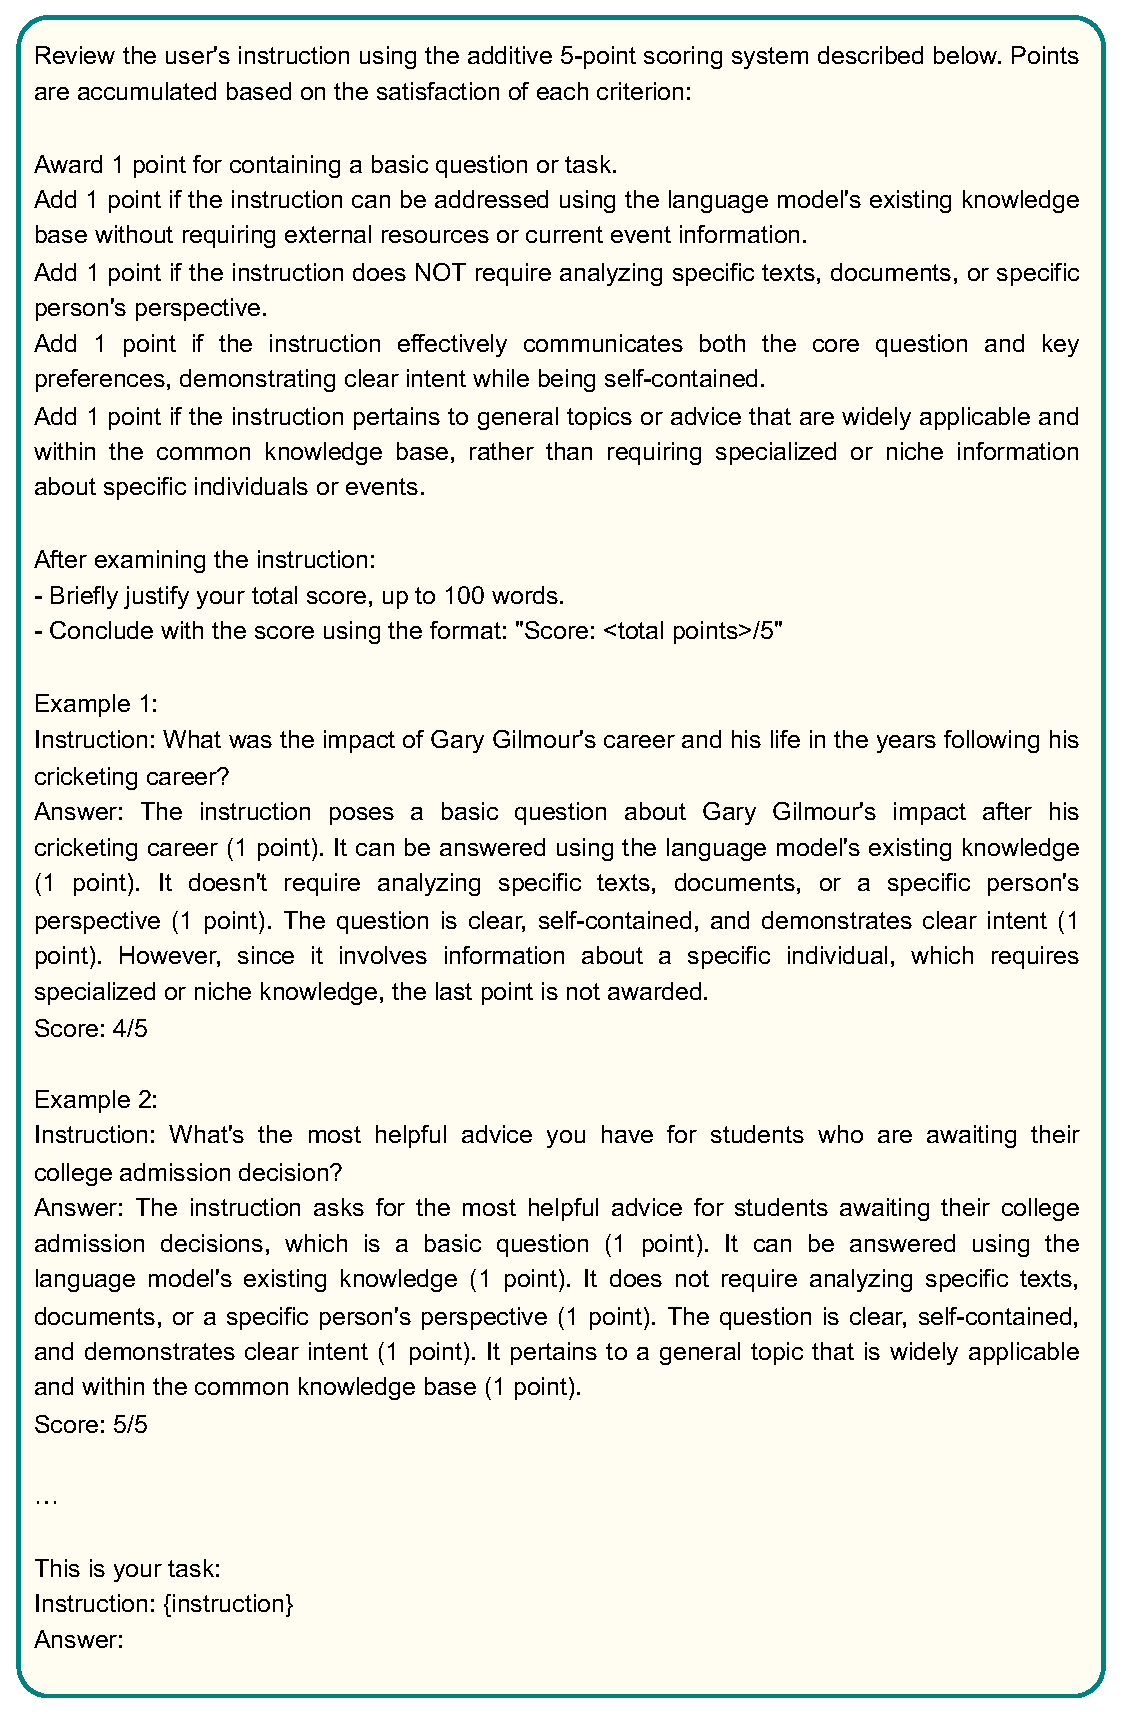
\includegraphics[width=0.8\linewidth]{source/prompt/prompt_ins_score.pdf}
\caption{Prompt for scoring initial instructions.}
\label{figure:prompt_ins_score}
\end{figure}

\begin{figure}[ht]
\centering
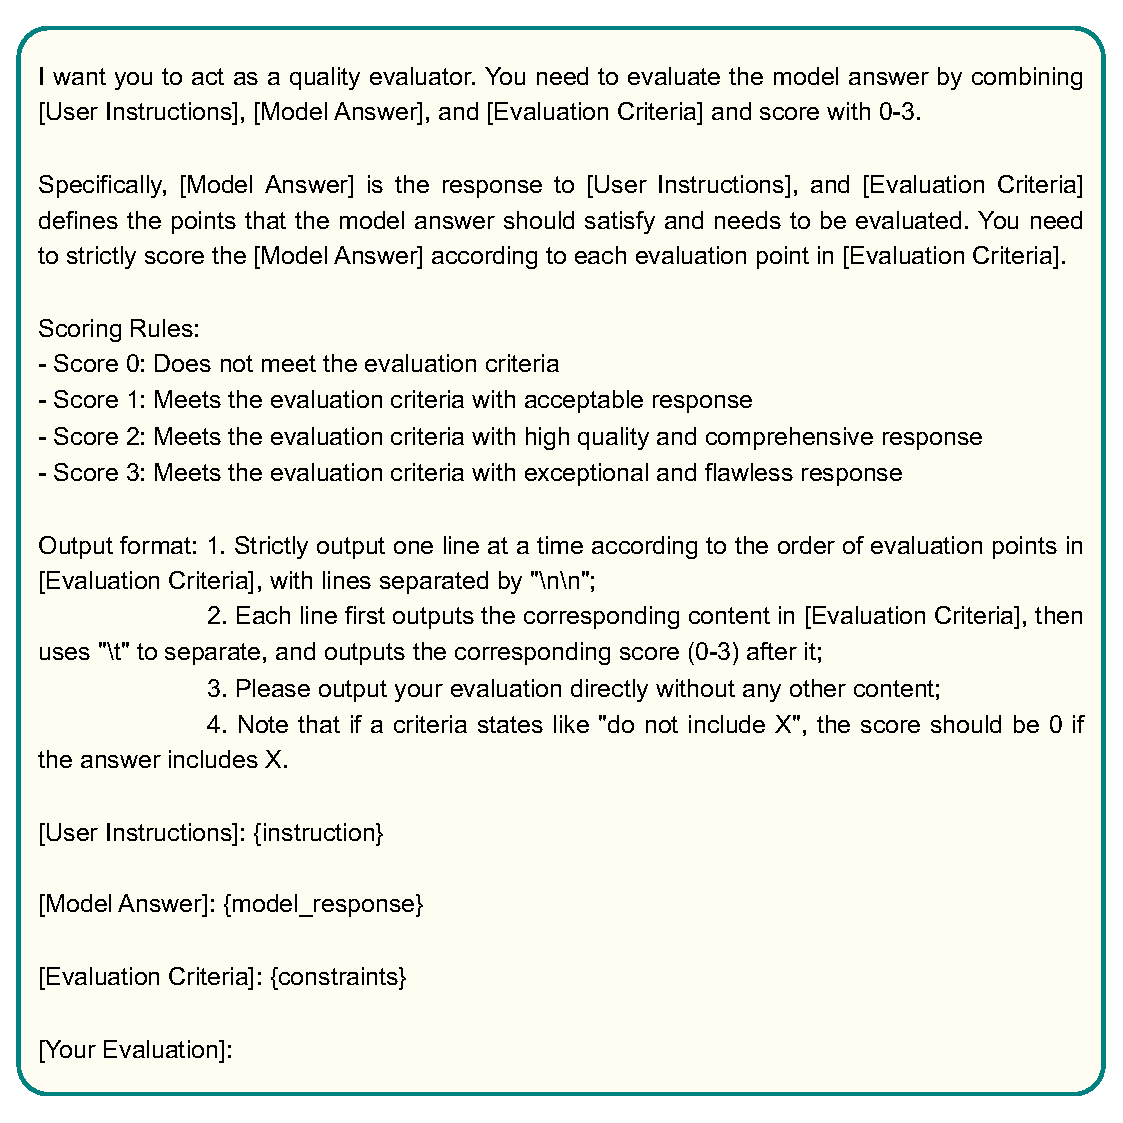
\includegraphics[width=0.8\linewidth]{source/prompt/cons_check.pdf}
\caption{Prompt for verifying model responses against constraints.}
\label{figure:cons_check}
\end{figure}

\begin{figure}[ht]
\centering
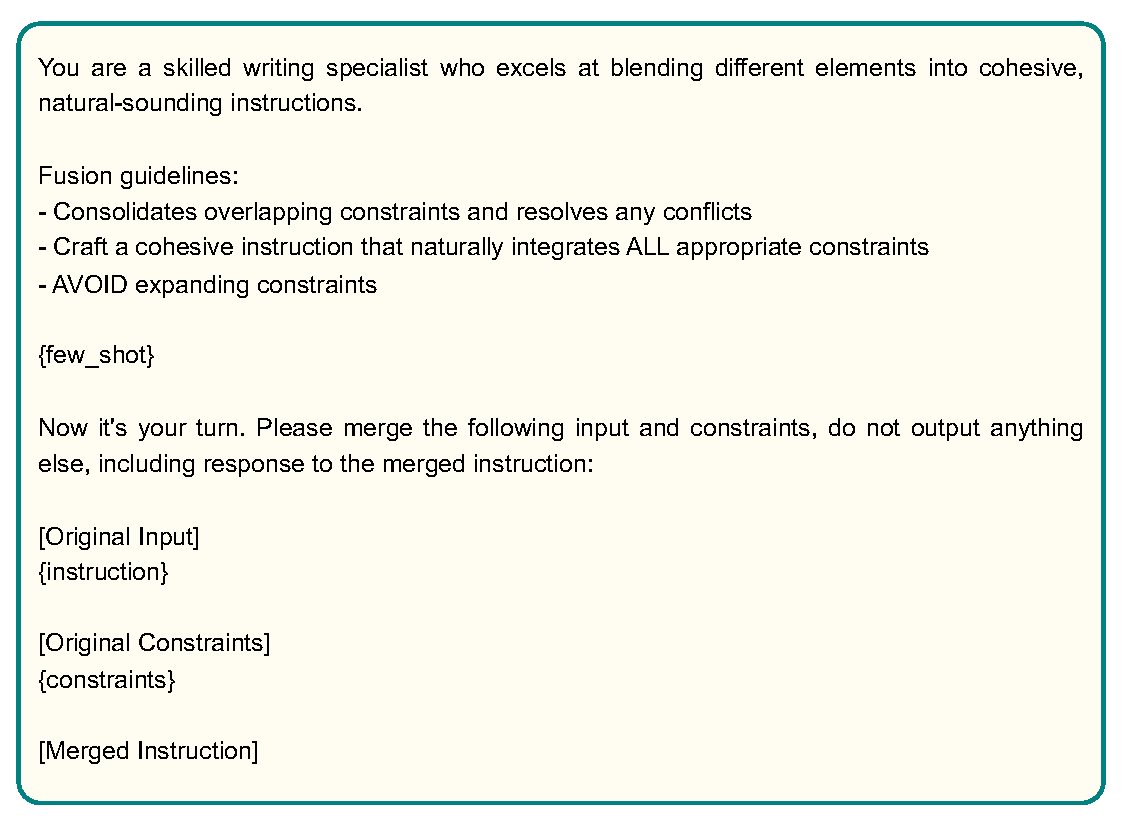
\includegraphics[width=0.8\linewidth]{source/prompt/cons_combine.pdf}
\caption{Prompt for combining instructions with constraints.}
\label{figure:cons_combine}
\end{figure}



% Add author contributions with \credit{} after authorship is confirmed.
% \printcredits

\bibliographystyle{cas-model2-names}
\bibliography{main}

\end{document}
